\documentclass[12pt,a4paper]{article}
\usepackage{booktabs,amsmath,amssymb,longtable,array,xcolor,microtype}
\usepackage{geometry}
\geometry{margin=2.5cm}
% ── Cross-references to main.tex ──────────────────────────────────────────
% Build order: xelatex main → xelatex suppl_wrapper → xelatex suppl_wrapper
% The first pass reads main.aux (produced by main compilation).
% If main.aux is absent, refs will show ?? on first pass only.
\usepackage{xr}
\externaldocument{main}   % reads main.aux from the same build directory
\usepackage{hyperref}
% ─────────────────────────────────────────────────────────────────────────
% macros_structural.tex -- structural constants shared between main paper and supplementary.
% Use % macros_structural.tex -- structural constants shared between main paper and supplementary.
% Use % macros_structural.tex -- structural constants shared between main paper and supplementary.
% Use \input{macros_structural} in both main.tex and macros.tex.
% Defined with \providecommand (idempotent: second \input is a no-op).
% One definition per name — no duplicates.
\providecommand{\Ncand}{473}
\providecommand{\Nexcl}{84}
\providecommand{\Nvia}{389}
\providecommand{\Ntrios}{1{,}944{,}653}
\providecommand{\dmin}{10}
\providecommand{\kk}{3}
\providecommand{\Fmmsize}{181}
\providecommand{\FAsize}{213}
\providecommand{\FAinter}{132}
\providecommand{\ndraws}{500}
\providecommand{\nboot}{2{,}000}
% E1 bootstrap uses B=10,000 (diag_e1b_greedy.py, default_rng(42)); all others use \nboot
\providecommand{\nbootEone}{10{,}000}
\providecommand{\Tset}{\mathcal{T}}
\providecommand{\Fset}{\mathcal{F}}
 in both main.tex and macros.tex.
% Defined with \providecommand (idempotent: second \input is a no-op).
% One definition per name — no duplicates.
\providecommand{\Ncand}{473}
\providecommand{\Nexcl}{84}
\providecommand{\Nvia}{389}
\providecommand{\Ntrios}{1{,}944{,}653}
\providecommand{\dmin}{10}
\providecommand{\kk}{3}
\providecommand{\Fmmsize}{181}
\providecommand{\FAsize}{213}
\providecommand{\FAinter}{132}
\providecommand{\ndraws}{500}
\providecommand{\nboot}{2{,}000}
% E1 bootstrap uses B=10,000 (diag_e1b_greedy.py, default_rng(42)); all others use \nboot
\providecommand{\nbootEone}{10{,}000}
\providecommand{\Tset}{\mathcal{T}}
\providecommand{\Fset}{\mathcal{F}}
 in both main.tex and macros.tex.
% Defined with \providecommand (idempotent: second \input is a no-op).
% One definition per name — no duplicates.
\providecommand{\Ncand}{473}
\providecommand{\Nexcl}{84}
\providecommand{\Nvia}{389}
\providecommand{\Ntrios}{1{,}944{,}653}
\providecommand{\dmin}{10}
\providecommand{\kk}{3}
\providecommand{\Fmmsize}{181}
\providecommand{\FAsize}{213}
\providecommand{\FAinter}{132}
\providecommand{\ndraws}{500}
\providecommand{\nboot}{2{,}000}
% E1 bootstrap uses B=10,000 (diag_e1b_greedy.py, default_rng(42)); all others use \nboot
\providecommand{\nbootEone}{10{,}000}
\providecommand{\Tset}{\mathcal{T}}
\providecommand{\Fset}{\mathcal{F}}

% AUTO-GENERATED by scripts/generate_macros_amplitudes.py -- DO NOT EDIT BY HAND
% source: results/amplitudes/amplitudes.json  sha256=234f6e1c2697ea54
% Re-generate: uv run python scripts/generate_macros_amplitudes.py
%
% All rho_j = 1/L2(mm_norm(x_j)) (rho_shift formula).
% TV_W = E1-W formula (section 6.4). TV(alpha=2) uses def-(ii): w^2*A^2.

% --- TV decomposition (SAW, alpha=1) ---
\newcommand{\TVvec}{0.3113}           % TV_vec (rho_shift; was 0.315 rho_raw)
\newcommand{\TVBvec}{0.2479}          % between-group TV
\newcommand{\TVWvec}{0.1954}          % within-group TV (E1-W formula)
\newcommand{\TVrnk}{0.091}             % TV under midranks normalization

% --- TV(alpha=2) -- manuscript formula w_j^2*A_j^2 (definition ii) ---
\newcommand{\TValphaTwo}{0.673}         % TV(2) vector (def-ii; NOT 0.590=def-i)
\newcommand{\DeltaTValphaTwo}{0.362}    % TV(2)-TV(1) vector
\newcommand{\TValphaTwoMM}{0.160}        % TV(2) min-max (A_j=1 baseline)

% --- Perm inflation ---
\newcommand{\PermInflation}{2.86}        % w_eff(perm)/w(perm)
\newcommand{\IntraGperm}{1.56}           % rho_perm/Abar_G1
\newcommand{\UrbanRatioVec}{0.53}       % w_eff(urban)/w(urban) under vec (deflation: < 1)
\newcommand{\AspectRatioVec}{0.51}      % w_eff(aspect)/w(aspect) under vec (deflation: < 1)
\newcommand{\AspectAmplitudeRatio}{1.77}  % rho_aspect/rho_asp_flip = sqrt(n_nonleeward/n_leeward)
\newcommand{\RnkContinuousGainPct}{12.1}  % % gain of 7 fully continuous criteria under midranks

% --- delta norms (for §6.8 using rho_shift) ---
\newcommand{\DeltaLtwoshift}{0.3101}       % ||delta||_2 = L2_vec (rho_shift)
\newcommand{\DeltaLinfshift}{0.2835}       % ||delta||_inf = max|w_eff_j - w_j| (rho_shift)

% --- rho_shift max change from rho_raw ---
\newcommand{\RhoShiftMaxPct}{4.3}        % max % diff rho_raw vs rho_shift
\newcommand{\RhoShiftMaxCrit}{coast}       % criterion with max diff

% --- Slope of optimal-assembly ordering (OLS on 3 normalisations) ---
\newcommand{\slopeOpt}{139.5}            % |slope| of Q2_opt vs TV_vec (was 137.7)

% --- Pole-coding counterfactuals (eq:vec paragraph) ---
% rho_j = 1/L2(X_via[:,j]) where X_via is from _build_decision_matrix.
% X_via[:,aspect] has leeward=1 (94 sites); flipped = leeward=0.
% X_via[:,perm] is the straight mm-norm; inverted = 1-mm_norm.
\newcommand{\RhoPerm}{0.583}             % 1/L2(mm_perm)  heavy-zero dist
\newcommand{\RhoPermInverted}{0.052}   % 1/L2(1-mm_perm) if inverted
\newcommand{\RhoAspect}{0.103}          % 1/sqrt(94)  leeward=1
\newcommand{\RhoAspectFlipped}{0.058}  % 1/sqrt(295) if leeward=0

% --- m_eff and concentration (generated, not hardcoded) ---
\newcommand{\meff}{4.03}             % effective number of criteria = (L1_delta)^2/(L2_delta)^2
\newcommand{\PermAbsDevPct}{45.5}  % perm share of |w_eff - w| (total absolute deviation)

% macros.tex — manually maintained macros NOT covered by auto-generated files.
%
% Auto-generated macro files (DO NOT edit by hand):
%   macros_amplitudes.tex  <- generate_macros_amplitudes.py  (TV*, rho*, slopeOpt, PermInflation)
%   macros_e6.tex          <- generate_macros_e6.py           (Esix* macros)
%   results/r1/macros_r1.tex <- generate_macros_r1.py         (Rone*, Rasp* macros)
%
% This file: mc_unified contrasts, E1, F1/F3/Q3/F8, assembly, structural constants.
% Values were last audited against CSV/JSON sources on 2026-10-xx.
% Forbidden values enforced by check_consistency.py.
%
% For orphan macros (no computable source), see comment above each entry.

% ── Contrastes principais (mc_unified.py, seed=42, B=10000, N=500) ────────────
\newcommand{\NormMainEffect}{34.6}       % C1 all4 (34.55 rounds to 34.6)
\newcommand{\NormGreedyContrast}{25.4}   % C6 greedy-only
\newcommand{\AsmMain}{-1.1}              % C2 all4 (-1.05 rounds to -1.1)
\newcommand{\AsmMM}{8.1}                 % C4 within mm

% Kappa=200 informative cells defined in macros_structural.tex — not duplicating here

% ── Contrastes κ=50 (robustez; bootstrap emparelhado, B=2000, seed=43) ────────
% Source: results/bootstrap_k50_k200.csv (2026-10-28)
\newcommand{\NormGreedyContrastKfifty}{29.2}     % Norm greedy κ=50
\newcommand{\NormGreedyContrastKfiftyLo}{25.7}
\newcommand{\NormGreedyContrastKfiftyHi}{33.0}
\newcommand{\NormInfoEffectKfifty}{33.2}          % Norm informative κ=50
\newcommand{\NormInfoEffectKfiftyLo}{29.4}
\newcommand{\NormInfoEffectKfiftyHi}{36.7}
\newcommand{\AggContrastKfifty}{+20.4}            % Agg pooled κ=50 (SAW-TOPSIS, SIG)
\newcommand{\AggLoKfifty}{17.7}
\newcommand{\AggHiKfifty}{23.3}
\newcommand{\AsmMMtopsisKfifty}{2.4}              % Asm mm TOPSIS κ=50 (n.s.)
\newcommand{\AsmMMtopsisKfiftyLo}{-0.4}
\newcommand{\AsmMMtopsisKfiftyHi}{5.2}
\newcommand{\AsmVecKfifty}{0.7}                   % Asm vec mean κ=50 (n.s.)
\newcommand{\AsmVecKfiftyLo}{-1.5}
\newcommand{\AsmVecKfiftyHi}{3.0}
\newcommand{\InteractionTOPSISKfifty}{3.4}        % Interaction TOPSIS κ=50 (n.s.)
\newcommand{\InteractionTOPSISKfiftyLo}{-0.4}
\newcommand{\InteractionTOPSISKfiftyHi}{7.4}
\newcommand{\AggContrast}{-0.4}
\newcommand{\AggLo}{-2.1}
\newcommand{\AggHi}{+1.3}
\newcommand{\TOSTp}{0.010}               % TOST p, delta=2.5pp, 3-cell

% Assembly por sub-celula
\newcommand{\AsmMMtopsis}{2.2}
\newcommand{\AsmMMtopsisLo}{0.2}
\newcommand{\AsmMMtopsisHi}{4.2}
\newcommand{\AsmVecSAW}{9.4}
\newcommand{\AsmVecSAWLo}{12.4}          % magnitude; sinal negativo no texto
\newcommand{\AsmVecSAWHi}{6.4}
\newcommand{\AsmVecTOPSIS}{11.0}
\newcommand{\AsmVecTOPSISLo}{14.2}
\newcommand{\AsmVecTOPSISHi}{7.8}
\newcommand{\AsmVec}{10.2}               % media SAW/vec e TOP/vec (magnitude)
\newcommand{\AsmVecLo}{13.6}             % CI media (de all_contrasts.py C5)
\newcommand{\AsmVecHi}{7.0}

% Normalizacao informativa e interaccao (celulas informativas, excl. SAW/mm/opt)
\newcommand{\NormInfoEffect}{31.7}
\newcommand{\NormInfoLo}{27.7}
\newcommand{\NormInfoHi}{35.7}
\newcommand{\AsmThreecell}{-6.1}
\newcommand{\AsmThreecellLo}{-8.1}
\newcommand{\AsmThreecellHi}{-4.1}
\newcommand{\InteractionTOPSIS}{13.2}
\newcommand{\InteractionTOPSISLo}{9.6}
\newcommand{\InteractionTOPSISHi}{17.0}

% ── Marco A: E1 intervention results ────────────────────────────────────
% EoneWloss and EoneVloss generated by generate_macros_e1.py (read from log).
% AUTO-GENERATED by scripts/generate_macros_e1.py -- DO NOT EDIT BY HAND
% source: data/e1_v3_rerun_20261002.log  sha256=e05cd8a4befdd8c5
% Original run: Athena, 500 draws, float64, eps=1e-9 (commit 44f7ff5)
% Cross-check: EoneVloss == 100 - QtwovecOptimal from wp3_mc_fixed_raw.csv

\newcommand{\EoneVloss}{43.2}            % 100 - Q2_opt(E1-V) = vector cell loss
\newcommand{\EoneWloss}{35.8}            % 100 - Q2_opt(E1-W) = within-group loss

% E1 P2 bootstrap (B=10000, default_rng(42), source: results/e1/e1_diag_bootstrap.csv sha=e6ee692cdeebd768):
% EonePtwoDiff = QtwoEoneWOpt - QtwoEoneVOpt = 64.2 - 56.8; CI from bootstrap
% Note: old text had [3.8, 11.0] — not reproducible; corrected to [4.0, 11.0] (default_rng)
\newcommand{\EonePtwoDiff}{7.4}       % W exceeds V by this many pp (point estimate)
\newcommand{\EonePtwoBootCILo}{4.0}   % 95% paired bootstrap CI lower bound
\newcommand{\EonePtwoBootCIHi}{11.0}  % 95% paired bootstrap CI upper bound

% ── TV(alpha=2) — manuscript formula w_j^eff(2) = w_j^2 * A_j^2 / sum w_k^2*A_k^2 ──
% Source: results/amplitudes/amplitudes.json (generate_macros_amplitudes.py).
% MOVED to macros_amplitudes.tex: TValphaTwo, DeltaTValphaTwo, EsixTargetTVW
% (EsixTargetTVW is now generated by generate_macros_e6.py from CSV target_tvw column)
% TVBvec, TVWvec, slopeOpt also moved to macros_amplitudes.tex.

% ── Marco A: Mechanism 1 prediction for admissible-only cell ────────────
% REMOVED 2026-10-01: MechOnePredAdmiss, MechOneShare, MismatchRatioHi,
% MismatchRatioLo were based on 80 pp attributed to reference-set mismatch.
% That result was an artefact of inconsistent aspect coding in build_score_473.
% Audit: DEV-E4-007 (corpus/PRESPEC_E4.md). These macros are now prohibited
% in check_consistency.py (see rule: forbidden_macros_e4).
%\newcommand{\MechOnePredAdmiss}{14.7}
%\newcommand{\MechOneShare}{18}
%\newcommand{\MismatchRatioHi}{5.4}
%\newcommand{\MismatchRatioLo}{0.34}

% ── Marco A: tab:tvorder values ─────────────────────────────────────────
\newcommand{\QtwommGreedy}{86.0}
\newcommand{\QtwommOptimal}{100.0}
\newcommand{\QtwovecGreedy}{66.2}
\newcommand{\QtwovecOptimal}{56.8}
\newcommand{\QtwoRanksGreedy}{86.0}
\newcommand{\QtwoRanksOptimal}{88.2}
% TOPSIS Q2 from factorial (mc_unified_raw.csv, N=500, kappa=200)
\newcommand{\QtwoTOPSISmmGrd}{94.4}
\newcommand{\QtwoTOPSISmmOpt}{96.6}
\newcommand{\QtwoTOPSISvecGrd}{63.4}
\newcommand{\QtwoTOPSISvecOpt}{52.4}
% D6: SE for tab:factorial Q2 values (SE = sqrt(p(1-p)/500)*100, 1dp)
\newcommand{\QtwoSEmmGreedy}{1.6}        % SAW/mm/grd
\newcommand{\QtwoSEmmOptimal}{0.0}       % SAW/mm/opt: exact by Prop 1 (SE=0)
\newcommand{\QtwoSEvecGreedy}{2.1}       % SAW/vec/grd
\newcommand{\QtwoSEvecOptimal}{2.2}      % SAW/vec/opt
\newcommand{\QtwoSETOPSISmmGrd}{1.0}     % TOPSIS/mm/grd
\newcommand{\QtwoSETOPSISmmOpt}{0.8}     % TOPSIS/mm/opt
\newcommand{\QtwoSETOPSISvecGrd}{2.2}    % TOPSIS/vec/grd
\newcommand{\QtwoSETOPSISvecOpt}{2.2}    % TOPSIS/vec/opt
% Bootstrap CI for greedy normalisation contrast (from mc_unified.py B=2000)
\newcommand{\NormGreedyContrastLo}{21.2}
\newcommand{\NormGreedyContrastHi}{29.7}

% ── TV values — MOVED to macros_amplitudes.tex (see that file) ─────────
% TVvec, PermInflation, RhoShiftMaxPct, RhoShiftMaxCrit now in macros_amplitudes.tex
% [MOVED to macros_amplitudes.tex] TVrnk (now generated from canonical scorer)
% \TVvecNumerical is PROHIBITED (check_consistency): same as \TVvec now.

% ── LossTabTVorder (used in supplementary) ──────────────────────────────
\newcommand{\LossTabTVorder}{19.8}       % mm_greedy - vec_greedy = 86.0 - 66.2

% ── SAWgreedyContrast (used in supplementary) ───────────────────────────
\newcommand{\SAWgreedyContrast}{19.8}    % 86.0 - 66.2

% ── §8.6: WP3 five-level regression (moved to supplementary) ────────────
\newcommand{\slopeFive}{93.0}
\newcommand{\SEfive}{6.8}
\newcommand{\dffive}{3}
\newcommand{\SxxPctVecFive}{73}
\newcommand{\RsqDropFrom}{0.984}
\newcommand{\RsqDropTo}{0.397}
\newcommand{\slopeDropSum}{30.9}
\newcommand{\pDropSum}{0.18}


% ── Marco B: E4 preparation values (from tvw_e4.py, commit d4e970b) ─────
% [MOVED to macros_amplitudes.tex] IntraGperm
\newcommand{\TVWrw}{0.082}       % TV_W for E4 R-W cell (0.0815 rounded to 3 s.f.)

% ── Marco B/E2: TV_W for directional patterns (computed 2026-10-01) ─────
\newcommand{\TVWrj}{0.082}       % TV_W(r_j pattern = R-W): 0.0815 rounded
\newcommand{\TVWinvrj}{0.085}    % TV_W(1/r_j pattern = R-V'): 0.0852 rounded
% Cost of r_j pattern: 0 pp (R-V* opt = 100%); cost of 1/r_j: 11.6 pp (R-V' opt = 88.4%)
\newcommand{\RVstarOptimal}{100.0}   % R-V* kappa=200 optimal (consistent coding)
\newcommand{\RVstarGreedy}{97.8}     % R-V* kappa=200 greedy  (consistent coding)
\newcommand{\RVoptimal}{6.2}         % R-V  kappa=200 optimal (continuous aspect, 473-base) [corrected 2026-10-28]
\newcommand{\RVgreedy}{6.4}          % R-V  kappa=200 greedy  (continuous aspect, 473-base) [corrected 2026-10-28]
\newcommand{\RVprimeOptimal}{88.4}   % R-V' kappa=200 optimal (1/r_j pattern vs A')
\newcommand{\RefSetGreedyGain}{11.8} % R1-2: greedy improvement with consistent coding (pp)

% ── Marco B/E3: aspect non-monotonicity (recomputed 2026-10-26 with correct geographic formula)
\newcommand{\AspSpearman}{-0.445}    % Spearman(normalised azimuth, leeward indicator)
\newcommand{\AspSpearmanP}{0.000}    % p-value (strongly anti-correlated, p<0.001)
\newcommand{\AspTopQuartile}{100}    % sites in top 25% continuous aspect
\newcommand{\AspTopQuartileNonLee}{100} % of which indicator=0 (non-leeward), %
\newcommand{\AspLeewardCount}{94}    % indicator=1 (leeward [90-180]) sites (invariant)
\newcommand{\AspLeewardPct}{24.2}    % % of 389 viable sites that are leeward

% ── F1: SAW-TOPSIS contrast by stratum (aggregation_strata.py, 2026-10-02) ──
\newcommand{\AggContrastPooled}{-0.4}  % 3-cell pooled: -0.4 pp (excl Prop 1 cell)
\newcommand{\AggContrastPooledLo}{-2.0} % 95% CI lower
\newcommand{\AggContrastPooledHi}{1.2}  % 95% CI upper
\newcommand{\AggStratumMMgrd}{-8.4}    % minmax/greedy: SAW-TOPSIS pp (SIG)
\newcommand{\AggStratumMMgrdAbs}{8.4}  % |AggStratumMMgrd|; TOPSIS exceeds SAW by this in mm/grd
\newcommand{\AggStratumVecgrd}{2.8}    % vector/greedy: SAW-TOPSIS pp (SIG)
\newcommand{\AggStratumMMopt}{3.4}     % minmax/optimal: SAW-TOPSIS pp (SIG)
\newcommand{\AggStratumVecopt}{4.4}    % vector/optimal: SAW-TOPSIS pp (SIG)

% ── Fase D / R1 results (from results/r1/macros_r1.tex) ──────────────────────
\newcommand{\RoneOneOptDelta}{0.0}      % R1-1 opt: Δ_ref optimal (pp)
\newcommand{\RoneTwoGrdDelta}{11.8}     % R1-2 grd: Δ_ref greedy (pp)
\newcommand{\RoneTwoGrdCIlo}{8.8}      % R1-2 grd CI lower (pp)
\newcommand{\RoneTwoGrdCIhi}{14.8}     % R1-2 grd CI upper (pp)
\newcommand{\RaspOptimal}{15.6}        % R-asp opt: aspect continuous cell (%) [corrected 2026-10-26]
\newcommand{\RaspGreedy}{15.8}         % R-asp grd (%) [corrected 2026-10-26]
\newcommand{\RaspLoss}{84.4}           % = 100 - \RaspOptimal (one decimal precision)
% Residual reference-set effect (R-asp vs R-V, source: results/r1/r1_bootstrap.csv)
% [corrected 2026-10-28: R-V recomputed with geographic azimuth convention]
\newcommand{\ResidualRefOptDelta}{9.4}    % R-asp vs R-V opt pp
\newcommand{\ResidualRefOptCIlo}{6.6}     % 95\% CI lower
\newcommand{\ResidualRefOptCIhi}{12.4}    % 95\% CI upper
\newcommand{\ResidualRefGrdDelta}{9.4}    % R-asp vs R-V grd pp [corrected 2026-10-28]
\newcommand{\ResidualRefGrdCIlo}{6.4}     % 95\% CI lower
\newcommand{\ResidualRefGrdCIhi}{12.6}    % 95\% CI upper


% ── F3: Q3 results (q3_perdraw.py v2, 2026-10-19) ───────────────────────────
% Corrected: script now uses verbatim saw_sc/topsis_sc from mc_2cube_fixed.py.
% Assertions: q2==1=>gap==0 passes in all 8 cells (0 violations, N=500).
% Coincidence SAW/vec == TOP/vec: 47.2% (greedy), 70.4% (optimal) -- below 90%.
\newcommand{\QthreeSAWmmOpt}{0.000}       % Q3 SAW/mm/opt (=0, Q2=100%)
\newcommand{\QthreeSAWmmGrd}{0.0018}      % Q3 SAW/mm/grdy  (unchanged)
\newcommand{\QthreeSAWvecGrd}{0.0086}     % Q3 SAW/vec/grdy  (was 0.0216, bug fixed)
\newcommand{\QthreeSAWvecOpt}{0.0087}     % Q3 SAW/vec/opt   (was 0.0212, bug fixed)
\newcommand{\QthreeTOPSISmmGrd}{0.0009}   % Q3 TOPSIS/mm/grdy  (0.000879, unchanged at 4dp)
\newcommand{\QthreeTOPSISmmOpt}{0.0005}   % Q3 TOPSIS/mm/opt   (0.000478, unchanged at 4dp)
\newcommand{\QthreeTOPSISvecGrd}{0.0114}  % Q3 TOPSIS/vec/grdy (was 0.447, bug fixed)
\newcommand{\QthreeTOPSISvecOpt}{0.0111}  % Q3 TOPSIS/vec/opt  (was 0.447, bug fixed)
% All 8 Q3 values computed vs min-max reference frontier.
% Empirically: gap==0 iff q2==1 on every draw in every cell (N=500).
% This is an observed regularity; weak dominance remains theoretically
% possible when two non-dominated portfolios differ in only one criterion.

% Q3 in percent of attainable range (Q3_mean * 100, 2dp)
\newcommand{\QthreeSAWmmGrdPct}{0.18}
\newcommand{\QthreeSAWmmOptPct}{0.00}
\newcommand{\QthreeSAWvecGrdPct}{0.86}
\newcommand{\QthreeSAWvecOptPct}{0.87}
\newcommand{\QthreeTOPSISmmGrdPct}{0.09}
\newcommand{\QthreeTOPSISmmOptPct}{0.05}
\newcommand{\QthreeTOPSISvecGrdPct}{1.14}
\newcommand{\QthreeTOPSISvecOptPct}{1.11}

% Conditional gap = Q3 / (1-Q2), mean shortfall when portfolio misses frontier (%)
\newcommand{\CondGapSAWmmGrd}{1.29}
\newcommand{\CondGapSAWvecGrd}{2.54}
\newcommand{\CondGapSAWvecOpt}{2.01}
\newcommand{\CondGapTOPSISmmGrd}{1.57}
\newcommand{\CondGapTOPSISmmOpt}{1.40}
\newcommand{\CondGapTOPSISvecGrd}{3.11}
\newcommand{\CondGapTOPSISvecOpt}{2.34}


% ── Structural macros (shared with main.tex preamble via macros_structural.tex) ─
% One definition per name; providecommand is idempotent so \input is safe twice.
% macros_structural.tex -- structural constants shared between main paper and supplementary.
% Use % macros_structural.tex -- structural constants shared between main paper and supplementary.
% Use \input{macros_structural} in both main.tex and macros.tex.
% Defined with \providecommand (idempotent: second \input is a no-op).
% One definition per name — no duplicates.
\providecommand{\Ncand}{473}
\providecommand{\Nexcl}{84}
\providecommand{\Nvia}{389}
\providecommand{\Ntrios}{1{,}944{,}653}
\providecommand{\dmin}{10}
\providecommand{\kk}{3}
\providecommand{\Fmmsize}{181}
\providecommand{\FAsize}{213}
\providecommand{\FAinter}{132}
\providecommand{\ndraws}{500}
\providecommand{\nboot}{2{,}000}
% E1 bootstrap uses B=10,000 (diag_e1b_greedy.py, default_rng(42)); all others use \nboot
\providecommand{\nbootEone}{10{,}000}
\providecommand{\Tset}{\mathcal{T}}
\providecommand{\Fset}{\mathcal{F}}
 in both main.tex and macros.tex.
% Defined with \providecommand (idempotent: second \input is a no-op).
% One definition per name — no duplicates.
\providecommand{\Ncand}{473}
\providecommand{\Nexcl}{84}
\providecommand{\Nvia}{389}
\providecommand{\Ntrios}{1{,}944{,}653}
\providecommand{\dmin}{10}
\providecommand{\kk}{3}
\providecommand{\Fmmsize}{181}
\providecommand{\FAsize}{213}
\providecommand{\FAinter}{132}
\providecommand{\ndraws}{500}
\providecommand{\nboot}{2{,}000}
% E1 bootstrap uses B=10,000 (diag_e1b_greedy.py, default_rng(42)); all others use \nboot
\providecommand{\nbootEone}{10{,}000}
\providecommand{\Tset}{\mathcal{T}}
\providecommand{\Fset}{\mathcal{F}}


% ── F1 per-cell aggregation contrasts (SAW-TOPSIS, aggregation_strata.csv) ───
\newcommand{\AggMMgrdCIlo}{-11.6}
\newcommand{\AggMMgrdCIhi}{-5.2}
\newcommand{\AggVecgrdCIlo}{0.4}
\newcommand{\AggVecgrdCIhi}{5.2}
\newcommand{\AggMMoptCIlo}{1.8}
\newcommand{\AggMMoptCIhi}{5.0}
\newcommand{\AggVecoptCIlo}{2.0}
\newcommand{\AggVecoptCIhi}{6.8}


% ── F8: circularidade do benchmark (compute_f8_circularity.py, 2026-10-02) ───
% Frontier built with VECTOR objectives; 4 SAW cells; N=500, kappa=200
\newcommand{\FEightVecOptQ}{100.0}   % SAW/vec/opt with vec frontier (Prop1 ✓)
\newcommand{\FEightVecOptSE}{0.0}
\newcommand{\FEightMMOptQ}{94.4}    % SAW/mm/opt with vec frontier
\newcommand{\FEightMMOptSE}{1.0}
\newcommand{\FEightMMOptLoss}{5.6}  % 100 - FEightMMOptQ: loss vs vec frontier
% Aspect pole-coding comparison (compute_aspect_polecoding.py, TOPSIS/vec, 389 sites)
% Paper had 0.960/0.960 — both were wrong (copy error); correct values below.
\newcommand{\AspectTauB}{0.92}        % Kendall tau_b between leeward=1 vs leeward=0 orderings
\newcommand{\AspectTopKAgree}{0.94}   % top-100 set agreement fraction
\newcommand{\FEightVecGrdQ}{100.0}  % SAW/vec/greedy with vec frontier (empirical; 457/500 same portfolio as optimal)
\newcommand{\FEightMMGrdQ}{72.4}    % SAW/mm/greedy with vec frontier
% Interpretation: vec/opt=100% confirmed with Prop1 (Theorem 1) in commit 43b8427.
% Previous commit 9cdceb4 gave 89.4% due to double-normalisation bug (injection approach
% caused aspect misclassification); replaced with direct vec objectives in commit 4d0a98d.

% Raw sensitivity macros moved to macros_raw_sens.tex (AUTO-GENERATED).
% See scripts/generate_macros_raw_sens.py


% AUTO-GENERATED by scripts/generate_macros_raw_sens.py -- DO NOT EDIT BY HAND
% source: raw_sensitivity_4cells.csv sha256=9aee31af4d3e8d47
% source: raw_sensitivity_q2.json sha256=9aee31af4d3e8d47

\newcommand{\RawSensSawOptSame}{488}  % SAW/optimal shift==raw (true form)
\newcommand{\RawSensSawGrdSame}{489}  % SAW/greedy shift==raw (true form)
\newcommand{\RawSensSame}{488}  % SAW/optimal (kept for backwards compat)
\newcommand{\RawSensTotal}{500}  % total draws
\newcommand{\RawSensTopsisOptSame}{487}  % TOPSIS/optimal shift==raw
\newcommand{\RawSensTopsisGrdSame}{489}  % TOPSIS/greedy shift==raw
\newcommand{\RawSensTopsisOptDiff}{13}  % TOPSIS/optimal shift!=raw
\newcommand{\RawSensTopsisGrdDiff}{11}  % TOPSIS/greedy shift!=raw
\newcommand{\RawSensMaxDeltaQtwo}{1.0}  % max |delta Q2| across 4 cells (pp)

% AUTO-GENERATED by scripts/generate_macros_e6.py -- DO NOT EDIT BY HAND
% source: results/e6/e6_raw_prespec.csv  sha256=c330ccc00640c966
% Naming convention: CamelCase, \Esix prefix, family suffix (Logn/Beta/Unif/Zinf/All)
% commit hash stored in results/e6/e6_stats.json (not here, to keep output deterministic)

% ── Parametric dispatchers ───────────────────────────────────────────
% ── Parametric dispatchers (for use as \EsixPthreeP{Logn}, \EsixPfourP{All}, etc.) ──
% Guards: undefined suffix -> compile-time error (not silent \relax)
\newcommand{\EsixPthreeP}[1]{%
  \ifcsname EsixPthreeP#1\endcsname\csname EsixPthreeP#1\endcsname
  \else\errmessage{E6 macro EsixPthreeP#1 undefined}\fi}
\newcommand{\EsixPfourP}[1]{%
  \ifcsname EsixPfourP#1\endcsname\csname EsixPfourP#1\endcsname
  \else\errmessage{E6 macro EsixPfourP#1 undefined}\fi}

\newcommand{\EsixTargetTVW}{0.199}  % E6 pre-registered TV_W target (0.1986 rho_raw era; see DEV-E6-005)

% ── Design ───────────────────────────────────────────────────────────
\newcommand{\EsixNinst}{120}  % total instances (4 families x 30 reps)
\newcommand{\EsixNfam}{4}  % number of marginal families
\newcommand{\EsixNcells}{7}  % number of experimental cells
\newcommand{\EsixNperdraw}{200}  % draws per instance-cell pair
\newcommand{\EsixNdraws}{24{,}000}  % draws per cell (120 inst x 200 draws)
\newcommand{\EsixNdrawsTotal}{168{,}000}  % total draws across all 7 cells
\newcommand{\EsixPiZinf}{0.90}  % zero-inflation rate for zero_inflated family

% ── P1 ──────────────────────────────────────────────────────────────
\newcommand{\EsixPoneHits}{48{,}000}  % draws with TV_W=0 and Q2^opt=100%
\newcommand{\EsixPoneTotal}{48{,}000}  % total M+B cell draws (= 2 x EsixNdraws)
\newcommand{\EsixPoneNDesign}{24{,}000}  % draws per baseline cell (= 120 inst x 200 draws)

% ── P2 (conservative; Poisson-binomial null) ───────────────────────
% denominator = instances with loss>0 at some TV_W level (L/F/H)
% primary count = L>=F>=H AND H<L (= monotone excl. 3-way ties)
% null: p_i=1/6 (n_distinct=3), 1/3 (n_distinct=2), 0 (n_distinct=1)
\newcommand{\EsixPtwoLossyNLogn}{20}  % instances with any loss
\newcommand{\EsixPtwoMonoLogn}{19}  % L>=F>=H AND H<L (monotone excl. 3-way ties)
\newcommand{\EsixPtwoTiesLogn}{1}  % 3-way ties L=F=H (counted as failures)
\newcommand{\EsixPtwoReversalLogn}{0}  % L>=F>=H fails
\newcommand{\EsixPtwoStrictOnlyLogn}{15}  % sensitivity: n_distinct=3 AND L>=F>=H AND H<L
\newcommand{\EsixPtwoPLogn}{p<0.001}  % Poisson-binomial one-sided (mixed p_i=1/6 or 1/3)

\newcommand{\EsixPtwoLossyNBeta}{18}  % instances with any loss
\newcommand{\EsixPtwoMonoBeta}{17}  % L>=F>=H AND H<L (monotone excl. 3-way ties)
\newcommand{\EsixPtwoTiesBeta}{0}  % 3-way ties L=F=H (counted as failures)
\newcommand{\EsixPtwoReversalBeta}{1}  % L>=F>=H fails
\newcommand{\EsixPtwoStrictOnlyBeta}{6}  % sensitivity: n_distinct=3 AND L>=F>=H AND H<L
\newcommand{\EsixPtwoPBeta}{p<0.001}  % Poisson-binomial one-sided (mixed p_i=1/6 or 1/3)

\newcommand{\EsixPtwoLossyNUnif}{22}  % instances with any loss
\newcommand{\EsixPtwoMonoUnif}{22}  % L>=F>=H AND H<L (monotone excl. 3-way ties)
\newcommand{\EsixPtwoTiesUnif}{0}  % 3-way ties L=F=H (counted as failures)
\newcommand{\EsixPtwoReversalUnif}{0}  % L>=F>=H fails
\newcommand{\EsixPtwoStrictOnlyUnif}{9}  % sensitivity: n_distinct=3 AND L>=F>=H AND H<L
\newcommand{\EsixPtwoPUnif}{p<0.001}  % Poisson-binomial one-sided (mixed p_i=1/6 or 1/3)

\newcommand{\EsixPtwoLossyNZinf}{28}  % instances with any loss
\newcommand{\EsixPtwoMonoZinf}{27}  % L>=F>=H AND H<L (monotone excl. 3-way ties)
\newcommand{\EsixPtwoTiesZinf}{1}  % 3-way ties L=F=H (counted as failures)
\newcommand{\EsixPtwoReversalZinf}{0}  % L>=F>=H fails
\newcommand{\EsixPtwoStrictOnlyZinf}{22}  % sensitivity: n_distinct=3 AND L>=F>=H AND H<L
\newcommand{\EsixPtwoPZinf}{p<0.001}  % Poisson-binomial one-sided (mixed p_i=1/6 or 1/3)

\newcommand{\EsixPtwoLossyNAll}{88}  % instances with any loss
\newcommand{\EsixPtwoMonoAll}{85}  % L>=F>=H AND H<L (monotone excl. 3-way ties)
\newcommand{\EsixPtwoTiesAll}{2}  % 3-way ties L=F=H (counted as failures)
\newcommand{\EsixPtwoReversalAll}{1}  % L>=F>=H fails
\newcommand{\EsixPtwoStrictOnlyAll}{52}  % sensitivity: n_distinct=3 AND L>=F>=H AND H<L
\newcommand{\EsixPtwoPAll}{p<0.001}  % Poisson-binomial one-sided (mixed p_i=1/6 or 1/3)

% ── P3 ──────────────────────────────────────────────────────────────
% pre-registered: V_inf_F <= W_inf_F (TV_B agrava perda)
\newcommand{\EsixPthreeInfPminFam}{0.08}  % min per-family one-sided binomial p (informative)

\newcommand{\EsixPthreePreregNLogn}{24}  % instances meeting pre-registered criterion V<=W
\newcommand{\EsixPthreeDenomLogn}{30}  % total instances tested (30 or 120)
\newcommand{\EsixPthreeInfStrictLogn}{13}  % informative strict V<W
\newcommand{\EsixPthreeInfDenomLogn}{19}  % informative denominator
\newcommand{\EsixPthreePLogn}{p=0.084}  % one-sided binomial p (informative)

\newcommand{\EsixPthreePreregNBeta}{28}  % instances meeting pre-registered criterion V<=W
\newcommand{\EsixPthreeDenomBeta}{30}  % total instances tested (30 or 120)
\newcommand{\EsixPthreeInfStrictBeta}{7}  % informative strict V<W
\newcommand{\EsixPthreeInfDenomBeta}{9}  % informative denominator
\newcommand{\EsixPthreePBeta}{p=0.090}  % one-sided binomial p (informative)

\newcommand{\EsixPthreePreregNUnif}{22}  % instances meeting pre-registered criterion V<=W
\newcommand{\EsixPthreeDenomUnif}{30}  % total instances tested (30 or 120)
\newcommand{\EsixPthreeInfStrictUnif}{8}  % informative strict V<W
\newcommand{\EsixPthreeInfDenomUnif}{16}  % informative denominator
\newcommand{\EsixPthreePUnif}{p=0.598}  % one-sided binomial p (informative)

\newcommand{\EsixPthreePreregNZinf}{24}  % instances meeting pre-registered criterion V<=W
\newcommand{\EsixPthreeDenomZinf}{30}  % total instances tested (30 or 120)
\newcommand{\EsixPthreeInfStrictZinf}{8}  % informative strict V<W
\newcommand{\EsixPthreeInfDenomZinf}{14}  % informative denominator
\newcommand{\EsixPthreePZinf}{p=0.395}  % one-sided binomial p (informative)

\newcommand{\EsixPthreePreregNAll}{98}  % instances meeting pre-registered criterion V<=W
\newcommand{\EsixPthreeDenomAll}{120}  % total instances tested (30 or 120)
\newcommand{\EsixPthreeInfStrictAll}{36}  % informative strict V<W
\newcommand{\EsixPthreeInfDenomAll}{58}  % informative denominator
\newcommand{\EsixPthreePAll}{p=0.043}  % one-sided binomial p (informative)

% ── P4 (bilateral; post hoc pooling across families = All) ─────────
% deflate > inflate is the OPPOSITE of the prediction (DEV-E6-003)
\newcommand{\EsixPfourDeflLogn}{13}  % deflate>inflate strictly (OPPOSITE of prediction)
\newcommand{\EsixPfourInflLogn}{12}  % inflate>deflate strictly (prediction direction)
\newcommand{\EsixPfourNonTiedLogn}{25}  % non-tied pairs (denominator for binomtest)
\newcommand{\EsixPfourTiedLogn}{5}  % tied pairs (excluded from binomtest)
\newcommand{\EsixPfourPLogn}{p=1.000}  % two-sided binomial
\newcommand{\EsixPfourPropLogn}{0.52}  % proportion Defl/NonTied (2dp)
\newcommand{\EsixPfourPropThreeLogn}{0.520}  % proportion Defl/NonTied (3dp)
\newcommand{\EsixPfourCIloLogn}{0.33}  % Wilson 95% CI lower (2dp)
\newcommand{\EsixPfourCIhiLogn}{0.70}  % Wilson 95% CI upper (2dp)

\newcommand{\EsixPfourDeflBeta}{12}  % deflate>inflate strictly (OPPOSITE of prediction)
\newcommand{\EsixPfourInflBeta}{4}  % inflate>deflate strictly (prediction direction)
\newcommand{\EsixPfourNonTiedBeta}{16}  % non-tied pairs (denominator for binomtest)
\newcommand{\EsixPfourTiedBeta}{14}  % tied pairs (excluded from binomtest)
\newcommand{\EsixPfourPBeta}{p=0.077}  % two-sided binomial
\newcommand{\EsixPfourPropBeta}{0.75}  % proportion Defl/NonTied (2dp)
\newcommand{\EsixPfourPropThreeBeta}{0.750}  % proportion Defl/NonTied (3dp)
\newcommand{\EsixPfourCIloBeta}{0.51}  % Wilson 95% CI lower (2dp)
\newcommand{\EsixPfourCIhiBeta}{0.90}  % Wilson 95% CI upper (2dp)

\newcommand{\EsixPfourDeflUnif}{10}  % deflate>inflate strictly (OPPOSITE of prediction)
\newcommand{\EsixPfourInflUnif}{8}  % inflate>deflate strictly (prediction direction)
\newcommand{\EsixPfourNonTiedUnif}{18}  % non-tied pairs (denominator for binomtest)
\newcommand{\EsixPfourTiedUnif}{12}  % tied pairs (excluded from binomtest)
\newcommand{\EsixPfourPUnif}{p=0.815}  % two-sided binomial
\newcommand{\EsixPfourPropUnif}{0.56}  % proportion Defl/NonTied (2dp)
\newcommand{\EsixPfourPropThreeUnif}{0.556}  % proportion Defl/NonTied (3dp)
\newcommand{\EsixPfourCIloUnif}{0.34}  % Wilson 95% CI lower (2dp)
\newcommand{\EsixPfourCIhiUnif}{0.75}  % Wilson 95% CI upper (2dp)

\newcommand{\EsixPfourDeflZinf}{18}  % deflate>inflate strictly (OPPOSITE of prediction)
\newcommand{\EsixPfourInflZinf}{10}  % inflate>deflate strictly (prediction direction)
\newcommand{\EsixPfourNonTiedZinf}{28}  % non-tied pairs (denominator for binomtest)
\newcommand{\EsixPfourTiedZinf}{2}  % tied pairs (excluded from binomtest)
\newcommand{\EsixPfourPZinf}{p=0.185}  % two-sided binomial
\newcommand{\EsixPfourPropZinf}{0.64}  % proportion Defl/NonTied (2dp)
\newcommand{\EsixPfourPropThreeZinf}{0.643}  % proportion Defl/NonTied (3dp)
\newcommand{\EsixPfourCIloZinf}{0.46}  % Wilson 95% CI lower (2dp)
\newcommand{\EsixPfourCIhiZinf}{0.79}  % Wilson 95% CI upper (2dp)

\newcommand{\EsixPfourDeflAll}{53}  % deflate>inflate strictly (OPPOSITE of prediction)
\newcommand{\EsixPfourInflAll}{34}  % inflate>deflate strictly (prediction direction)
\newcommand{\EsixPfourNonTiedAll}{87}  % non-tied pairs (denominator for binomtest)
\newcommand{\EsixPfourTiedAll}{33}  % tied pairs (excluded from binomtest)
\newcommand{\EsixPfourPAll}{p=0.053}  % two-sided binomial, post hoc pooling (DEV-E6-003)
\newcommand{\EsixPfourPropAll}{0.61}  % proportion Defl/NonTied (2dp)
\newcommand{\EsixPfourPropThreeAll}{0.609}  % proportion Defl/NonTied (3dp)
\newcommand{\EsixPfourCIloAll}{0.50}  % Wilson 95% CI lower (2dp)
\newcommand{\EsixPfourCIhiAll}{0.71}  % Wilson 95% CI upper (2dp)


% E6 Q2 loss by family at \EsixTargetTVW (condition W_inf_F, from principal CSV)
% zero_inflated: q2_mean=0.8932 => loss=10.7 pp
\newcommand{\EsixLossZinfWinfF}{10.7}  % Q2 loss Zinf at W_inf_F (approx)

% ── Sensitivity macros (DEV-E6-005; target TW_F=0.1954) ───────────────
% AUTO-GENERATED by scripts/generate_macros_e6.py -- DO NOT EDIT BY HAND
% source: results/e6/sensit/e6_raw_sensit_tvwF01954.csv  sha256=0a8dfc528140d8bf

\newcommand{\EsixSensTargetTVW}{0.1954}  % sensitivity run TW_F (rho_shift / Fogo corrected; DEV-E6-005)

\newcommand{\EsixSensPfourDeflAll}{51}  % sensit: deflate>inflate strictly
\newcommand{\EsixSensPfourInflAll}{32}  % sensit: inflate>deflate strictly
\newcommand{\EsixSensPfourNonTiedAll}{83}  % sensit: non-tied pairs (denominator)
\newcommand{\EsixSensPfourTiedAll}{37}  % sensit: tied pairs
\newcommand{\EsixSensPfourPAll}{p=0.048}  % sensit: two-sided binomial p-value
\newcommand{\EsixSensPfourPropAll}{0.61}  % sensit: deflate proportion (2dp)
\newcommand{\EsixSensPfourPropThreeAll}{0.614}  % sensit: deflate proportion (3dp)
\newcommand{\EsixSensPfourCIloAll}{0.51}  % sensit: Wilson 95% CI lower (2dp)
\newcommand{\EsixSensPfourCIhiAll}{0.71}  % sensit: Wilson 95% CI upper (2dp)

\newcommand{\EsixSensPoneHits}{48000}  % sensit P1: draws on frontier
\newcommand{\EsixSensPoneTotal}{48000}  % sensit P1: total M+B draws

\newcommand{\EsixSensPtwoMonoAll}{85}  % sensit P2: L>=F>=H AND H<L
\newcommand{\EsixSensPtwoLossyNAll}{88}  % sensit P2: informative instances
\newcommand{\EsixSensPtwoPAll}{p<0.001}  % sensit P2: Poisson-binomial p

\newcommand{\EsixSensPthreePreregNAll}{99}  % sensit P3: V<=W instances
\newcommand{\EsixSensPthreeDenomAll}{120}  % sensit P3: denominator
\newcommand{\EsixSensPthreeInfStrictAll}{36}  % sensit P3: strict V<W
\newcommand{\EsixSensPthreeInfDenomAll}{57}  % sensit P3: informative denom
\newcommand{\EsixSensPthreePAll}{p=0.031}  % sensit P3: one-sided binomial p

% P3 and P4 per family (sensitivity, for tab:e6-sens)
\newcommand{\EsixSensPthreePreregNLogn}{25}  % sensit P3 V<=W Logn
\newcommand{\EsixSensPthreeDenomLogn}{30}  % sensit P3 denom Logn
\newcommand{\EsixSensPthreeInfStrictLogn}{13}  % sensit P3 strict V<W Logn
\newcommand{\EsixSensPthreeInfDenomLogn}{18}  % sensit P3 informative denom Logn
\newcommand{\EsixSensPthreePLogn}{p=0.048}  % sensit P3 p Logn
\newcommand{\EsixSensPfourDeflLogn}{13}  % sensit P4 Defl Logn
\newcommand{\EsixSensPfourNonTiedLogn}{25}  % sensit P4 NonTied Logn
\newcommand{\EsixSensPfourPropThreeLogn}{0.520}  % sensit P4 prop Logn
\newcommand{\EsixSensPfourCIloLogn}{0.33}  % sensit P4 CI lo Logn
\newcommand{\EsixSensPfourCIhiLogn}{0.70}  % sensit P4 CI hi Logn
\newcommand{\EsixSensPfourPLogn}{p=1.000}  % sensit P4 p Logn

\newcommand{\EsixSensPthreePreregNBeta}{27}  % sensit P3 V<=W Beta
\newcommand{\EsixSensPthreeDenomBeta}{30}  % sensit P3 denom Beta
\newcommand{\EsixSensPthreeInfStrictBeta}{6}  % sensit P3 strict V<W Beta
\newcommand{\EsixSensPthreeInfDenomBeta}{9}  % sensit P3 informative denom Beta
\newcommand{\EsixSensPthreePBeta}{p=0.254}  % sensit P3 p Beta
\newcommand{\EsixSensPfourDeflBeta}{12}  % sensit P4 Defl Beta
\newcommand{\EsixSensPfourNonTiedBeta}{16}  % sensit P4 NonTied Beta
\newcommand{\EsixSensPfourPropThreeBeta}{0.750}  % sensit P4 prop Beta
\newcommand{\EsixSensPfourCIloBeta}{0.51}  % sensit P4 CI lo Beta
\newcommand{\EsixSensPfourCIhiBeta}{0.90}  % sensit P4 CI hi Beta
\newcommand{\EsixSensPfourPBeta}{p=0.077}  % sensit P4 p Beta

\newcommand{\EsixSensPthreePreregNUnif}{23}  % sensit P3 V<=W Unif
\newcommand{\EsixSensPthreeDenomUnif}{30}  % sensit P3 denom Unif
\newcommand{\EsixSensPthreeInfStrictUnif}{8}  % sensit P3 strict V<W Unif
\newcommand{\EsixSensPthreeInfDenomUnif}{15}  % sensit P3 informative denom Unif
\newcommand{\EsixSensPthreePUnif}{p=0.500}  % sensit P3 p Unif
\newcommand{\EsixSensPfourDeflUnif}{9}  % sensit P4 Defl Unif
\newcommand{\EsixSensPfourNonTiedUnif}{15}  % sensit P4 NonTied Unif
\newcommand{\EsixSensPfourPropThreeUnif}{0.600}  % sensit P4 prop Unif
\newcommand{\EsixSensPfourCIloUnif}{0.36}  % sensit P4 CI lo Unif
\newcommand{\EsixSensPfourCIhiUnif}{0.80}  % sensit P4 CI hi Unif
\newcommand{\EsixSensPfourPUnif}{p=0.607}  % sensit P4 p Unif

\newcommand{\EsixSensPthreePreregNZinf}{24}  % sensit P3 V<=W Zinf
\newcommand{\EsixSensPthreeDenomZinf}{30}  % sensit P3 denom Zinf
\newcommand{\EsixSensPthreeInfStrictZinf}{9}  % sensit P3 strict V<W Zinf
\newcommand{\EsixSensPthreeInfDenomZinf}{15}  % sensit P3 informative denom Zinf
\newcommand{\EsixSensPthreePZinf}{p=0.304}  % sensit P3 p Zinf
\newcommand{\EsixSensPfourDeflZinf}{17}  % sensit P4 Defl Zinf
\newcommand{\EsixSensPfourNonTiedZinf}{27}  % sensit P4 NonTied Zinf
\newcommand{\EsixSensPfourPropThreeZinf}{0.630}  % sensit P4 prop Zinf
\newcommand{\EsixSensPfourCIloZinf}{0.44}  % sensit P4 CI lo Zinf
\newcommand{\EsixSensPfourCIhiZinf}{0.78}  % sensit P4 CI hi Zinf
\newcommand{\EsixSensPfourPZinf}{p=0.248}  % sensit P4 p Zinf


% AUTO-GENERATED by scripts/generate_macros_f8.py -- DO NOT EDIT BY HAND
% source: f8_coincidence_v2.csv sha256=97152502b44bd610
% source: f8_vec_frontier.csv sha256=239133ce3ea7f6df
% Controls C1-C5 passed at generation time.

\newcommand{\FEightVecFrontierSize}{153}  % |F_vec| trios under AHP weights
\newcommand{\FEightVecCoinc}{457}  % vec/vec greedy==optimal (same portfolio)
\newcommand{\FEightVecSubopt}{43}  % vec/vec greedy!=optimal (empirical; not covered by Theorem 1)
\newcommand{\FEightMMCoinc}{201}  % vec/mm greedy==optimal
\newcommand{\FEightMMSubopt}{299}  % vec/mm greedy!=optimal
\newcommand{\FEightMMDivGrdOff}{111}  % vec/mm: opt ON, grd OFF (main pattern)
\newcommand{\FEightMMDivGrdOn}{1}  % vec/mm: grd ON, opt OFF (1 draw)


% ── F8 full 2×2 alignment matrix macros ──────────────────────────────────
% obj×score: VecVec=100%(Thm1), VecMM=94.4%, MMVec=99.8%(NEW), MMMM=100%(Thm1)
% Generated from: f8_circularity.csv (obj=vec) + f8_circularity_mm.csv (obj=mm)
% KEY RESULT: misalignment is strongly asymmetric.
%   VecMM/opt loss = 5.6 pp;  MMVec/opt loss = 0.2 pp (N=500 each)

% obj=vec frontier cells (existing)
\newcommand{\FEightVecVecOptQ}{100.0}  % obj=vec score=vec opt: Thm1 guarantee
\newcommand{\FEightVecMMOptQ}{94.4}   % obj=vec score=mm opt: main F8 result
\newcommand{\FEightVecMMOptSE}{1.028} % SE of above
\newcommand{\FEightVecMMOptLoss}{5.6} % 100-VecMMOptQ
\newcommand{\FEightVecVecGrdQ}{100.0}  % obj=vec score=vec grd: empirical 100%
\newcommand{\FEightVecMMGrdQ}{72.4}   % obj=vec score=mm grd
\newcommand{\FEightVecMMGrdSE}{1.999} % SE of above
\newcommand{\FEightVecMMGrdLoss}{27.6} % 100-VecMMGrdQ

% obj=mm frontier cells (NEW — from compute_f8_mm_frontier.py)
\newcommand{\FEightMmMMOptQ}{100.0}    % obj=mm score=mm opt: Thm1 guarantee
\newcommand{\FEightMmVecOptQ}{56.8}   % obj=mm score=vec opt: KEY RESULT
\newcommand{\FEightMmVecOptSE}{2.215} % SE of above
\newcommand{\FEightMmVecOptLoss}{43.2} % 100-MmVecOptQ
\newcommand{\FEightMmMMGrdQ}{86.0}    % obj=mm score=mm grd: ~factorial SAW/mm/grd
\newcommand{\FEightMmMMGrdSE}{1.552}  % SE of above
\newcommand{\FEightMmVecGrdQ}{66.2}   % obj=mm score=vec grd: KEY RESULT
\newcommand{\FEightMmVecGrdSE}{2.115} % SE of above
\newcommand{\FEightMmVecGrdLoss}{33.8} % 100-MmVecGrdQ


% ── Aligned misalignment losses (paired bootstrap B=2000, seed=777) ─────────
% Measure misalignment cost relative to the ALIGNED baseline in the same
% assembly strategy. Source: scripts/_f8_asymmetry_bootstrap.py.
% L1: optimal/mm-frontier  Q2(mm,mm,opt)-Q2(mm,vec,opt) = 100.0-56.8
\newcommand{\FEightOptMmLossVecScore}{43.2}
\newcommand{\FEightOptMmLossVecScoreLo}{38.6}
\newcommand{\FEightOptMmLossVecScoreHi}{47.8}
% L2: optimal/vec-frontier  Q2(vec,vec,opt)-Q2(vec,mm,opt) = 100.0-94.4
\newcommand{\FEightOptVecLossMmScore}{5.6}
\newcommand{\FEightOptVecLossMmScoreLo}{3.6}
\newcommand{\FEightOptVecLossMmScoreHi}{7.6}
% L3: greedy/mm-frontier  Q2(mm,mm,grd)-Q2(mm,vec,grd) = 86.0-66.2
% old \FEightMmVecGrdLoss = 33.8 was measured from 100%, not from 86.0%
\newcommand{\FEightGrdMmLossVecScore}{19.8}
\newcommand{\FEightGrdMmLossVecScoreLo}{14.6}
\newcommand{\FEightGrdMmLossVecScoreHi}{24.8}
% L4: greedy/vec-frontier  Q2(vec,vec,grd)-Q2(vec,mm,grd) = 100.0-72.4
\newcommand{\FEightGrdVecLossMmScore}{27.6}
\newcommand{\FEightGrdVecLossMmScoreLo}{23.6}
\newcommand{\FEightGrdVecLossMmScoreHi}{31.6}

% macros_e7.tex  --  E7 kappa sweep contrasts (authoritative run 2026-11-01)
% Source: results/e7/e7_contrasts.csv, B=2000, paired bootstrap
% Gates: 22/22 PASS (verify_e7_gates.py)
% All intervals are unadjusted; results are post hoc and descriptive.
% DO NOT edit manually -- regenerate with scripts/generate_macros_e7.py if needed.

% ── Agg_pooled3 (SAW-TOPSIS pooled, 3 informative cells) ──────────────────────
% k=50 and k=200 already in macros.tex (\AggContrastKfifty, \AggContrast)
\newcommand{\AggKtwentyfive}{+21.1}  % k=25  [18.5, 23.9]  SIG
\newcommand{\AggKtwentyfiveLo}{18.5}
\newcommand{\AggKtwentyfiveHi}{23.9}
\newcommand{\AggKonehundred}{+9.3}   % k=100 [7.1, 11.6]   SIG
\newcommand{\AggKonehundredLo}{7.1}
\newcommand{\AggKonehundredHi}{11.6}
\newcommand{\AggKfourhundred}{-5.7}  % k=400 [-7.3, -4.1]  SIG
\newcommand{\AggKfourhundredLo}{-7.3}
\newcommand{\AggKfourhundredHi}{-4.1}
\newcommand{\AggKthousand}{-9.0}     % k=1000 [-10.5, -7.5] SIG
\newcommand{\AggKthousandLo}{-10.5}
\newcommand{\AggKthousandHi}{-7.5}

% Update k=200 CI lo to match authoritative E7 (was -2.1 in macros.tex)
% \AggLo is defined in macros.tex as -2.1; the E7 final run gives -2.2.
% Difference is 0.1 pp (bootstrap sampling variability). No conclusion affected.
% The value in macros.tex is kept; update deferred to next full rerun.

% ── Norm_greedy (mm - vec, greedy) ────────────────────────────────────────────
% k=50 and k=200 already in macros.tex (\NormGreedyContrastKfifty, \NormGreedyContrast)
\newcommand{\NormKtwentyfive}{+21.0}   % k=25   [17.4, 24.4] SIG
\newcommand{\NormKonehundred}{+28.2}   % k=100  [24.2, 32.3] SIG
\newcommand{\NormKfourhundred}{+13.3}  % k=400  [9.3, 17.6]  SIG
\newcommand{\NormKthousand}{-3.5}      % k=1000 [-6.9, 0.2]  n.s.

% ── SAW mean across 3 informative cells (Q2 %, not contrast) ──────────────────
\newcommand{\SAWmeanKtwentyfive}{88.8}   % k=25   [86.6, 90.8]
\newcommand{\SAWmeanKfifty}{84.7}        % k=50   [82.4, 87.0]
\newcommand{\SAWmeanKonehundred}{77.4}   % k=100  [74.6, 80.2]
\newcommand{\SAWmeanKtwohundred}{69.7}   % k=200  [66.7, 72.6]
\newcommand{\SAWmeanKfourhundred}{69.0}  % k=400  [66.0, 71.8]
\newcommand{\SAWmeanKthousand}{70.3}     % k=1000 [67.8, 72.9]

% ── TOP mean across 3 informative cells (Q2 %, not contrast) ──────────────────
\newcommand{\TOPmeanKtwentyfive}{67.7}   % k=25   [64.8, 70.7]
\newcommand{\TOPmeanKfifty}{64.3}        % k=50   [61.3, 67.5]
\newcommand{\TOPmeanKonehundred}{68.1}   % k=100  [65.1, 71.1]
\newcommand{\TOPmeanKtwohundred}{70.1}   % k=200  [67.3, 72.9]
\newcommand{\TOPmeanKfourhundred}{74.7}  % k=400  [72.1, 77.2]
\newcommand{\TOPmeanKthousand}{79.3}     % k=1000 [77.4, 81.3]

% ── Asm_vec_SAW (optimal - greedy, SAW/vec) ───────────────────────────────────
% k=200 already in macros.tex (\AsmVecSAW = 9.4 magnitude, sign negative in text)
\newcommand{\AsmVecSAWKtwentyfive}{+3.4}   % k=25   [1.2, 5.8]    SIG
\newcommand{\AsmVecSAWKfifty}{+2.4}        % k=50   [-0.4, 5.2]   n.s.
\newcommand{\AsmVecSAWKonehundred}{-2.6}   % k=100  [-5.2, 0.0]   n.s.
\newcommand{\AsmVecSAWKfourhundred}{-23.6} % k=400  [-27.4, -20.0] SIG
\newcommand{\AsmVecSAWKthousand}{-38.4}    % k=1000 [-42.8, -34.0] SIG

% ── Asm_vec_TOP (optimal - greedy, TOPSIS/vec) ────────────────────────────────
% k=200 already in macros.tex (\AsmVecTOPSIS = 11.0 magnitude)
\newcommand{\AsmVecTOPKtwentyfive}{-2.0}   % k=25   [-5.6, 1.4]   n.s.
\newcommand{\AsmVecTOPKfifty}{-1.0}        % k=50   [-4.2, 2.4]   n.s.
\newcommand{\AsmVecTOPKonehundred}{-2.0}   % k=100  [-5.0, 1.0]   n.s.
\newcommand{\AsmVecTOPKfourhundred}{-19.6} % k=400  [-23.0, -16.2] SIG
\newcommand{\AsmVecTOPKthousand}{-40.8}    % k=1000 [-45.0, -36.2] SIG

% ── Magnitude helpers (for text "loses/improves X pp") ───────────────────────
% The sign-carrying macros above are used in signed contexts;
% these are for text that handles the direction verbally.
\newcommand{\AsmVecSAWKtwentyfiveMag}{3.4}   % k=25 positive (improves)
\newcommand{\AsmVecSAWKthousandMag}{38.4}     % k=1000 magnitude
\newcommand{\AsmVecTOPKthousandMag}{40.8}     % k=1000 magnitude

% kappa=inf (deterministic AHP weights) Q2 values for supplementary table
% Generated by scripts/kappa_inf.py
\newcommand{\QtwoInfSMiGre}{100}
\newcommand{\QtwoInfSMiOpt}{100}
\newcommand{\QtwoInfSVeGre}{100}
\newcommand{\QtwoInfSVeOpt}{0}
\newcommand{\QtwoInfTMiGre}{100}
\newcommand{\QtwoInfTMiOpt}{100}
\newcommand{\QtwoInfTVeGre}{100}
\newcommand{\QtwoInfTVeOpt}{0}

\begin{document}
\title{Supplementary Material}
\maketitle
\tableofcontents
\newpage
%% supplementary.tex
%% Content moved from main.tex (Marco A, 2026-10-01)
%% This file is NOT compiled with the main paper.
%% It contains sec:external (External validity: synthetic instances)
%% and tab:external (Synthetic grid table).
%%
%% To compile standalone, wrap with:
%%   \documentclass{article}
%%   \usepackage{booktabs,amsmath,amssymb}
%%   \begin{document}
%%   %% supplementary.tex
%% Content moved from main.tex (Marco A, 2026-10-01)
%% This file is NOT compiled with the main paper.
%% It contains sec:external (External validity: synthetic instances)
%% and tab:external (Synthetic grid table).
%%
%% To compile standalone, wrap with:
%%   \documentclass{article}
%%   \usepackage{booktabs,amsmath,amssymb}
%%   \begin{document}
%%   %% supplementary.tex
%% Content moved from main.tex (Marco A, 2026-10-01)
%% This file is NOT compiled with the main paper.
%% It contains sec:external (External validity: synthetic instances)
%% and tab:external (Synthetic grid table).
%%
%% To compile standalone, wrap with:
%%   \documentclass{article}
%%   \usepackage{booktabs,amsmath,amssymb}
%%   \begin{document}
%%   \input{supplementary}
%%   \end{document}

% =======================================================================
% =======================================================================
% \S7.7 External validity
% =======================================================================

\subsection{External validity: synthetic instances}
\label{sec:external}

The preceding sections quantify both mechanisms on a single candidate
set, Fogo Island, whose marginal distributions are specific and in one
respect extreme: \textit{perm} carries $350$ tied zeros.
This section separates the mechanism from the instance by re-drawing the
criterion columns while holding the spatial structure fixed: each
synthetic instance reuses the Fogo distance matrix, and hence the same
$\Ntrios$ feasible trios, and varies only the marginals.

\paragraph{Design.}
The manipulated factor is the \emph{number} of sparse criteria rather
than a global zero mass.
The reason is analytic: $\mathrm{TV}$ is invariant to a common amplitude
level (Section~\ref{sec:three_norms}), so applying the same zero mass to
every column leaves the elicited weights untouched however extreme that
mass becomes.
Distortion requires heterogeneity \emph{across} columns.
We therefore cross $n_{\mathrm{sparse}}\in\{0,1,2,3,4\}$, with zero mass
applied to the $n_{\mathrm{sparse}}$ most heavily weighted criteria,
with $p_0\in\{0.50,0.75,0.90,0.95\}$ and two tail shapes (lognormal,
bimodal), with $6$ replications: $240$ instances at $200$ draws each.
Four cells are evaluated per instance: SAW under min--max and vector
normalisation, each with greedy and optimal assembly.
The objectives $F_\ell$ are defined by min--max normalisation
throughout, so the vector cells measure score--evaluator divergence as
well as re-weighting.
The min--max/optimal cell is the regression test of
Proposition~\ref{prop:p1:stmt} and returned $Q_2=1$ in $240/240$
instances.

\paragraph{Unit of analysis.}
Replications within a cell are not independent draws of the manipulated
factor, so inference is conducted on the $20$ cell means.
The intra-class correlation is $\mathrm{ICC}=0.35$, giving a design
effect of $4.8$ and an effective sample size of
$n_{\mathrm{eff}}\approx50$ against the nominal $240$; reporting on
$240$ rows would understate the standard errors by roughly a factor
of two.

\paragraph{Total variation alone does not order the loss.}
Over all $20$ cells the loss correlates with $\mathrm{TV}$ at
$r=0.600$ ($95\%$ CI by Fisher transformation $[0.214,\,0.824]$,
$n=20$), but the relation is not monotone: $21.6\%$ of the $190$ cell
pairs are inversions (Kendall $\tau_b=0.550$).
Restricting to the $16$ cells that carry a distortion at all
($n_{\mathrm{sparse}}\ge1$), the association is statistically
indistinguishable from no effect ($r=0.346$, $p=0.189$): the
correlation over all $20$ cells is carried by the four cells in which
no criterion is sparse and the loss is zero by construction.
The inversions run in both directions of the design.
Holding $p_0$ fixed, the loss falls as the distortion is spread over
more criteria while $\mathrm{TV}$ does not fall correspondingly;
holding $n_{\mathrm{sparse}}=1$, the loss rises with $p_0$ up to
$0.90$ and then falls by $16.4$~pp at $p_0=0.95$ although
$\mathrm{TV}$ continues to rise.
Table~\ref{tab:external} reports both patterns by cell.

\paragraph{The factorisation does.}
Proposition~\ref{prop:concentration} accounts for this.
Regressing the loss on the $16$ distorted cells gives
$R^2_{\mathrm{adj}}=0.057$ for $\mathrm{TV}$ alone ($r=0.346$,
$p=0.189$, statistically indistinguishable from no effect)
against $R^2_{\mathrm{adj}}=0.488$ for $\lVert\delta\rVert_2$
of~\eqref{eq:l2fact} ($r=0.723$, $p=0.002$).
Entering magnitude and concentration separately gives
$R^2_{\mathrm{adj}}=0.582$ with a negative coefficient on
$m_{\mathrm{eff}}$ ($-0.026$ per effective criterion, $p=0.0008$): at
fixed $\mathrm{TV}$, spreading the distortion over more criteria
\emph{reduces} the loss, because deviations of opposite sign cancel in
the weighted sum.
The combined model, with both predictors, reaches $R^2_{\mathrm{adj}}=0.665$,
confirming that magnitude is necessary but not sufficient: concentration
is the term that $\mathrm{TV}$ omits.

\paragraph{What the grid does not establish.}
Under the two-group amplitude model the participation
ratio~\eqref{eq:meff} depends only on the total weight of the sparse
columns, so $m_{\mathrm{eff}}$ is constant within each level of
$n_{\mathrm{sparse}}$ and takes only the four values
$\{3.59,\,6.42,\,8.38,\,9.67\}$ across the grid
($\text{Spearman }\rho(m_{\mathrm{eff}},n_{\mathrm{sparse}})=1$).
Concentration was therefore not varied orthogonally to the manipulated
factor: the model in $\mathrm{TV}$ and $m_{\mathrm{eff}}$
($R^2_{\mathrm{adj}}=0.582$) is a reparameterisation of the model in
$\mathrm{TV}$ and $n_{\mathrm{sparse}}$ ($0.532$), and the
$5$-percentage-point gain reflects the concavity of the transformation
rather than independent information.
The factorisation~\eqref{eq:l2fact} is an algebraic identity and holds
for any deviation vector; what the grid supports is that the loss
responds to the combination of magnitude and concentration rather than
to magnitude alone, not that $m_{\mathrm{eff}}$ has been identified as
a separate causal channel.
A design in which the sparse columns carry unequal zero masses would
decouple the two, and is the natural next step.

\paragraph{Reconciliation with Fogo.}
Fogo has $m_{\mathrm{eff}}=4.05$ on the admissible range $[2,11]$,
placing it near the $n_{\mathrm{sparse}}=1$ regime of the grid
($m_{\mathrm{eff}}=3.59$).
The comparison must be made at the grid's estimand, which is the
greedy-assembly contrast under SAW: on Fogo that is
$86.0-66.2=19.8$~pp (min--max minus vector, greedy assembly,
Table~\ref{tab:tvorder}), not the
$\AggContrast$~pp normalisation main effect of Table~\ref{tab:contrasts}
(which averages both assemblies and both aggregations, and is therefore
attenuated by the optimal-assembly cells where min--max attains $100\%$
by Proposition~\ref{prop:p1:stmt}).
The model in $\lVert\delta\rVert_2$, fitted on the synthetic cells
alone, predicts $22.2$~pp at Fogo's $\lVert\delta\rVert_2=0.3127$, with
a $95\%$ prediction interval for a new instance of $[7.5,\,36.9]$~pp;
the model in $\mathrm{TV}$ predicts $14.0$~pp with interval
$[-4.7,\,32.7]$~pp.
Both prediction intervals contain the observed $19.8$~pp.
The $\lVert\delta\rVert_2$ point prediction exceeds the observed value
by $22.2-19.8=2.4$~pp; the TV-based prediction falls $5.8$~pp short
($14.0-19.8=-5.8$~pp).
We do not read the residuals as a calibrated bias in either direction.
The grid varies the marginals while holding the spatial structure fixed,
and its vector cells confound implicit re-weighting with
score--evaluator divergence because the objectives remain defined on
min--max throughout; Fogo's deviation geometry differs from the
generator's in a way the design does not parameterise
(see below).
What the grid establishes is that the loss responds to magnitude and
concentration jointly rather than to magnitude alone, and that Fogo's
predicted loss falls inside the interval the grid implies; it does not
establish a bound.

The shortfall is systematic and its source identifiable.
The generator inflates $n_{\mathrm{sparse}}$ columns and deflates the
remainder uniformly.
Fogo's deviation vector is not of that form: \textit{perm} is inflated
$2.88\times$ while \textit{urban} $(0.53\times)$, \textit{aspect}
$(0.51\times)$, \textit{aero} $(0.43\times)$ and \textit{wells}
$(0.40\times)$ are independently and unequally deflated
(Table~\ref{tab:amplitude}).
Two-sided distortion of this kind displaces the weight vector along the
simplex differently from a one-sided distortion of the same
$\lVert\delta\rVert_2$, so the generator does not reproduce Fogo's
deviation geometry.
We report the difference in geometry rather than a correction for it:
the grid supports the joint role of magnitude and concentration, and
does not calibrate the level of the loss for an instance outside its
generating family.

\begin{table*}[!t]
\centering
\caption{Synthetic grid: $20$ cells, $12$ instances each
  ($240$ instances, $200$ draws per instance).
  Loss is $Q_2(\text{min--max, greedy})-Q_2(\text{vector, greedy})$.
  $m_{\mathrm{eff}}$ is~\eqref{eq:meff} and $\lVert\delta\rVert_2$
  is~\eqref{eq:l2fact}, both reconstructed from the two-group amplitude
  model.
  Cells with $n_{\mathrm{sparse}}=0$ carry no distortion and are
  excluded from the regressions.
  Within each level of $p_0$ the loss falls as the distortion is spread
  over more criteria, while $\mathrm{TV}$ does not decline
  correspondingly and at $p_0=0.95$ peaks at $n_{\mathrm{sparse}}=2$;
  the two quantities are not ordered alike, which is what motivates
  Proposition~\ref{prop:concentration}.}
\label{tab:external}
\begin{tabular}{rrrrrr}
\toprule
$n_{\mathrm{sparse}}$ & $p_0$ & $\mathrm{TV}$ &
  $m_{\mathrm{eff}}$ & $\lVert\delta\rVert_2$ & Loss \\
\midrule
0 & --- & 0.007--0.008 & --- & --- & $\approx 0$ \\
1 & 0.50 & 0.121 & 3.59 & 0.128 & 0.065 \\
1 & 0.75 & 0.191 & 3.59 & 0.201 & 0.192 \\
1 & 0.90 & 0.262 & 3.59 & 0.276 & 0.360 \\
1 & 0.95 & 0.301 & 3.59 & 0.318 & 0.196 \\
2 & 0.50 & 0.165 & 6.42 & 0.130 & 0.105 \\
2 & 0.75 & 0.216 & 6.42 & 0.170 & 0.057 \\
2 & 0.90 & 0.307 & 6.42 & 0.242 & 0.146 \\
2 & 0.95 & 0.379 & 6.42 & 0.299 & 0.135 \\
3 & 0.50 & 0.160 & 8.38 & 0.110 & 0.065 \\
3 & 0.75 & 0.225 & 8.38 & 0.155 & 0.052 \\
3 & 0.90 & 0.303 & 8.38 & 0.210 & 0.129 \\
3 & 0.95 & 0.349 & 8.38 & 0.241 & 0.131 \\
4 & 0.50 & 0.153 & 9.67 & 0.099 & 0.025 \\
4 & 0.75 & 0.211 & 9.67 & 0.136 & 0.020 \\
4 & 0.90 & 0.269 & 9.67 & 0.173 & 0.058 \\
4 & 0.95 & 0.315 & 9.67 & 0.203 & 0.083 \\
\bottomrule
\end{tabular}
\end{table*}


% =======================================================================
% S6  Experiment E6 — Mechanism Generalisation: sensitivity analysis
% =======================================================================

\subsection*{Experiment E6 — Sensitivity to the TV\textsubscript{W} Target (DEV-E6-005)}
\label{sec:e6-sensit}

\noindent
The primary run used $\mathrm{TV}_W = \EsixTargetTVW$ for cell $W_\infty^F$
(the Fogo level computed with rho\_raw, before the rho\_shift correction).
The corrected level is $\EsixSensTargetTVW$ (difference $\approx 0.003$).
Both the amplitude cells $W_\infty^F$, $V_\infty^F$, and $W_{\mathrm{def}}^F$
use this target; cells M, B, $W_\infty^L$ and $W_\infty^H$ are identical
bit-for-bit between the two runs.

Table~\ref{tab:e6-sens} shows the P3 and P4 counts by family and pooled
for both runs.
P1 ($48{,}000/48{,}000$ in both) and P2 (Mono~$85/88$, $p<0.001$ in both)
are invariant across runs and are not repeated in the table.

\begin{table*}[!t]
\centering
\caption{P3 and P4 by marginal family and pooled, for the primary run
  ($\mathrm{TV}_W=\EsixTargetTVW$) and the sensitivity run
  ($\mathrm{TV}_W=\EsixSensTargetTVW$; DEV-E6-005).
  P3: met = V$_\infty^F \le$ W$_\infty^F$ (pre-registered);
  Strict = strict inequality among informative instances;
  $p$ = one-sided binomial.
  P4: Defl = deflate $>$ inflate (observed, opposite of prediction);
  Prop = Defl/NonTied; CI = Wilson 95\%; $p$ = two-sided binomial, post hoc.}
\label{tab:e6-sens}
\small
\begin{tabular}{lcccccccccc}
\toprule
& \multicolumn{4}{c}{Primary ($\mathrm{TV}_W=\EsixTargetTVW$)}
& \multicolumn{4}{c}{Sensitivity ($\mathrm{TV}_W=\EsixSensTargetTVW$)} \\
\cmidrule(lr){2-5}\cmidrule(lr){6-9}
Family
& \multicolumn{2}{c}{P3}
& \multicolumn{2}{c}{P4}
& \multicolumn{2}{c}{P3}
& \multicolumn{2}{c}{P4} \\
\cmidrule(lr){2-3}\cmidrule(lr){4-5}\cmidrule(lr){6-7}\cmidrule(lr){8-9}
& Strict/Inf & $p$ & Defl/Non & Prop ($p$) & Strict/Inf & $p$ & Defl/Non & Prop ($p$) \\
\midrule
Lognormal
& $\EsixPthreeInfStrictLogn/\EsixPthreeInfDenomLogn$ & $\EsixPthreeP{Logn}$
& $\EsixPfourDeflLogn/\EsixPfourNonTiedLogn$ & $\EsixPfourPropThreeLogn$ ($\EsixPfourP{Logn}$)
& $\EsixSensPthreeInfStrictLogn/\EsixSensPthreeInfDenomLogn$ & $\EsixSensPthreePLogn$
& $\EsixSensPfourDeflLogn/\EsixSensPfourNonTiedLogn$ & $\EsixSensPfourPropThreeLogn$ ($\EsixSensPfourPLogn$) \\
Beta(1,3)
& $\EsixPthreeInfStrictBeta/\EsixPthreeInfDenomBeta$ & $\EsixPthreeP{Beta}$
& $\EsixPfourDeflBeta/\EsixPfourNonTiedBeta$ & $\EsixPfourPropThreeBeta$ ($\EsixPfourP{Beta}$)
& $\EsixSensPthreeInfStrictBeta/\EsixSensPthreeInfDenomBeta$ & $\EsixSensPthreePBeta$
& $\EsixSensPfourDeflBeta/\EsixSensPfourNonTiedBeta$ & $\EsixSensPfourPropThreeBeta$ ($\EsixSensPfourPBeta$) \\
Uniform
& $\EsixPthreeInfStrictUnif/\EsixPthreeInfDenomUnif$ & $\EsixPthreeP{Unif}$
& $\EsixPfourDeflUnif/\EsixPfourNonTiedUnif$ & $\EsixPfourPropThreeUnif$ ($\EsixPfourP{Unif}$)
& $\EsixSensPthreeInfStrictUnif/\EsixSensPthreeInfDenomUnif$ & $\EsixSensPthreePUnif$
& $\EsixSensPfourDeflUnif/\EsixSensPfourNonTiedUnif$ & $\EsixSensPfourPropThreeUnif$ ($\EsixSensPfourPUnif$) \\
Zero-inflated
& $\EsixPthreeInfStrictZinf/\EsixPthreeInfDenomZinf$ & $\EsixPthreeP{Zinf}$
& $\EsixPfourDeflZinf/\EsixPfourNonTiedZinf$ & $\EsixPfourPropThreeZinf$ ($\EsixPfourP{Zinf}$)
& $\EsixSensPthreeInfStrictZinf/\EsixSensPthreeInfDenomZinf$ & $\EsixSensPthreePZinf$
& $\EsixSensPfourDeflZinf/\EsixSensPfourNonTiedZinf$ & $\EsixSensPfourPropThreeZinf$ ($\EsixSensPfourPZinf$) \\
\midrule
All (pooled)
& $\EsixPthreeInfStrictAll/\EsixPthreeInfDenomAll$ & $\EsixPthreeP{All}$
& $\EsixPfourDeflAll/\EsixPfourNonTiedAll$
& $\EsixPfourPropThreeAll$
  [$\EsixPfourCIloAll$,\,$\EsixPfourCIhiAll$]
  ($\EsixPfourP{All}$)
& $\EsixSensPthreeInfStrictAll/\EsixSensPthreeInfDenomAll$ & $\EsixSensPthreePAll$
& $\EsixSensPfourDeflAll/\EsixSensPfourNonTiedAll$
& $\EsixSensPfourPropThreeAll$
  [$\EsixSensPfourCIloAll$,\,$\EsixSensPfourCIhiAll$]
  ($\EsixSensPfourPAll$) \\
\bottomrule
\multicolumn{9}{l}{\footnotesize Strict/Inf = informative instances with strict $V<W$ / total informative. NonTied = non-tied pairs.}\\
\multicolumn{9}{l}{\footnotesize CI = Wilson 95\% confidence interval for the proportion. $p$ values for P4 are post hoc (DEV-E6-003).}\\
\end{tabular}
\end{table*}

% =======================================================================
% S0  Pre-registration for Experiment E1
% =======================================================================
%
% The following is PRESPEC_E1.md exactly as committed in f6042f8 on
% 2026-09-30T14:25:20-03:00, BEFORE any E1 run was executed.
% Commit subject: "prespec(E1): predictions declared before running --
%   P1=E1-B optimal=100%; P2=E1-W optimal~57%; P3=E1-B greedy~65%"
%
% File in repository: corpus/PRESPEC_E1.md at commit f6042f8
% Verify: git show f6042f8:corpus/PRESPEC_E1.md
%
% -----------------------------------------------------------------------

\section*{Pre-registered Predictions for Experiment~E1}
\label{sec:prespec_e1}

\noindent
\textbf{Committed:} 2026-09-30, commit \texttt{f6042f8}, before any E1 run.\\
\textbf{File:} \texttt{corpus/PRESPEC\_E1.md}.

\subsection*{Three predictions}

\begin{description}
\item[P1 (hard assertion)] \textbf{Cell~B optimal $= 100.0\%$.}
  By group-constant-amplitude sufficiency (Proposition~\ref{thm:groupconst}),
  $A_j = \bar A_g$ for all $j \in G_g$ implies the score is a strictly
  positive scalarisation of the group objectives; hence optimal assembly
  attains the frontier for any $w$.
  If P1 fails, there is a bug.

\item[P2 (primary empirical prediction)]
  $|Q_2^\text{W, optimal} - Q_2^\text{V, optimal}| < 5$~pp.\\
  \emph{Rationale:} both E1-W and E1-V have $\mathrm{TV}_W = 0.1986$.
  By the necessity argument, within-group distortion governs efficiency loss
  in optimal assembly; between-group distortion only displaces the optimum
  along the frontier.
  Predicted $Q_2^\text{W, optimal} \approx 57\%$ (close to E1-V's $56.8\%$).\\
  \emph{Falsification criterion:} if $Q_2^\text{W, optimal} > 90\%$,
  within-group distortion accounts for less than $10\%$ of the loss.

\item[P3 (secondary prediction)]
  $Q_2^\text{B, greedy} \neq 100.0\%$.\\
  \emph{Rationale:} greedy assembly is not constrained to be Pareto-efficient
  even under group-constant amplitudes; foreclosure affects greedy but not
  optimal.
  Predicted $Q_2^\text{B, greedy} \approx 65\%$.
\end{description}

\subsection*{Design}

Four score matrices differing only in $A_j$, with identical objectives,
frontier, draws, and feasible set ($\kappa=200$, $N=500$ draws, space $A'$):

\begin{center}
\begin{tabular}{llcc}
\toprule
Cell & $A_j$ & $\mathrm{TV}_B$ & $\mathrm{TV}_W$ \\
\midrule
M & $A_j \equiv 1$ (min--max)                        & 0       & 0 \\
B & $A_j = \bar A_g$ (between-group only)           & 0.2489  & 0 \\
W & $A_j \propto \rho_j/\bar A_g$ (within only)    & 0       & 0.1986 \\
V & $A_j = \rho_j$ (vector, as in WP3)             & 0.2489  & 0.1986 \\
\bottomrule
\end{tabular}
\end{center}

Groups and weighted means $\bar A_g$ (from \texttt{fogo\_constants.py}):
\begin{itemize}
\item $G_1 = \{\text{perm},\text{slope},\text{roads}\}$, indices $[0,1,2]$,
  $W_{G_1}=0.2950$, $\bar A_{G_1}=0.3731$.
\item $G_2 = \{\text{rivers},\text{aspect},\text{coast},\text{prot},\text{wells}\}$,
  indices $[3\ldots7]$, $W_{G_2}=0.3560$, $\bar A_{G_2}=0.1458$.
\item $G_3 = \{\text{urban},\text{aero},\text{cult}\}$, indices $[8,9,10]$,
  $W_{G_3}=0.3490$, $\bar A_{G_3}=0.1157$.
\end{itemize}

\subsection*{Outcome and deviations (DEV-E1-001 to DEV-E1-004)}

Results from \texttt{run\_e1\_v3.py}, commit \texttt{18e7a66}
(2026-09-30T23:23-03:00, Athena; reachable from G:\ after merge).

\begin{description}
\item[DEV-E1-001 INVALID] \texttt{380ee1a}, 2026-09-30T22:40-03:00.\\
  \emph{Fixed-objectives bug.}
  Script used objectives pre-computed on a fixed weight vector rather
  than per-draw objectives.
  Consequence: E1-V greedy $=100\%$ (should be $\sim54\%$, matching WP3);
  E1-W optimal $=100\%$ (should be $\sim57\%$, as predicted).
  Pre-registration \texttt{f6042f8} precedes this run in both the G: and
  Athena histories.

\item[DEV-E1-002 INVALID] \texttt{8391944}, 2026-09-30T23:11:38-03:00.\\
  \emph{Float32 dominance noise.}
  Per-draw objectives corrected, but float32 arithmetic introduced
  auto-dominance artefacts (same bug as WP3 greedy cells).
  Consequence: E1-V greedy $=14.8\%$ (expected $\sim54\%$).

\item[DEV-E1-003 INVALID] \texttt{18b7b88}, 2026-09-30T23:11:43-03:00.\\
  \emph{Score/objective normalisation mismatch.}
  Float64 applied but score computed over 473 sites while objectives
  evaluated over 389 admissible sites.
  Consequence: E1-V optimal $=46.6\%$ (expected $56.8\%$, regression
  test \textbf{FAIL}); E1-B optimal $=81.8\%$ (expected $100\%$, P1
  \textbf{FAIL}).

\item[DEV-E1-004] \texttt{18e7a66}, 2026-09-30T23:23:14-03:00.\\
  \emph{Corrected run (\texttt{run\_e1\_v3.py}): float64, eps$=10^{-9}$,
  score and objectives both over 389 admissible sites.}
  Results: \textbf{P1 confirmed} (E1-B optimal $=100\%$);
  \textbf{P2 falsified} at the pre-specified margin
  ($|Q_2^\text{W}-Q_2^\text{V}|=7.4$~pp, $95\%$ CI $[+3.8,+11.0]$,
  declared margin $<5$~pp);
  \textbf{P3 falsified} (D-greedy: greedy $=100\%$; post hoc diagnostic:
  score becomes nearly lexicographic in $F_1$, greedy and optimal
  coincide in $62.8\%$ of draws).
\end{description}




% =======================================================================
% S1  Pre-registration for Experiment E4
% =======================================================================
%
% Source: corpus/PRESPEC_E4.md
% Committed before any E4 run; deviations DEV-E4-001..007 appended
% chronologically as they occurred.
% Verify: git log --oneline corpus/PRESPEC_E4.md
%
% -----------------------------------------------------------------------

\section*{Pre-registered Design and Deviations for Experiment~E4}
\label{sec:prespec_e4}

\noindent
\textbf{Purpose:} Test whether the reference-set mismatch (473 vs.\ 389 sites
in the score) reduces to within-group re-weighting of the same form as
Experiment~E1, via the affine identity $n_j^{473}(a)=b_j+r_j\,n_j^{389}(a)$.

\subsection*{Pre-declared predictions}

\begin{description}
\item[P\_E4\_1 (Theorem, hard assertion)]
  Cells R-B and R-B$'$ attain $Q_2=100\%$ under optimal assembly on
  every draw.  Failure implies a bug or a violation of
  Theorem~\ref{thm:groupconst}.

\item[P\_E4\_2 (Regression test)]
  R-V (fwd) reproduces the published $473/A'$ cell within $3\,\mathrm{SE}$;
  R-V$'$ (mirror) reproduces the published $389/A$ cell within $3\,\mathrm{SE}$.

\item[P\_E4\_3 (Primary empirical, declared before any run)]
  Within-group loss $(100\%-Q_2^\text{R-W,opt})\ge 50\%$ of total loss
  $(100\%-Q_2^\text{R-V,opt})$ in the $473\to A'$ direction.

\item[P\_E4\_4 (Exploratory, declared)]
  The $80\,\mathrm{pp}$ vs.\ $5\,\mathrm{pp}$ asymmetry of
  tab:fourthcell persists in the within-group cells R-W and R-W$'$.

\item[P\_E4\_5 (Exploratory, declared, superseded by DEV-E4-004)]
  $Q_2^\text{R-W,opt} < Q_2^\text{E1-W,opt}=64.2\%$ despite
  $\mathrm{TV}_W(\text{R-W})=0.0815 < 0.199=\mathrm{TV}_W(\text{E1-W})$.
\end{description}

\subsection*{Deviations (DEV-E4-001 to DEV-E4-007)}

\begin{description}
\item[DEV-E4-001] \textit{Kappa/alpha parameter clarification.}
  The declared $\kappa=200$ is the Dirichlet concentration parameter
  (not the portfolio size $k=3$).  Two values $\kappa\in\{50,200\}$
  were run; the primary estimand uses $\kappa=200$.

\item[DEV-E4-002] \textit{Mirror direction frontier and amplitude sign.}
  The $389\to A$ direction uses the $A$-frontier (213 portfolios,
  objectives over 473 sites) and amplitude $A_j=1/r_j$ (not $r_j$).
  Corrected amplitude sentence: the 389-site score has amplitude $1/r_j$
  relative to the $A$-evaluator.

\item[DEV-E4-003] \textit{Weight-matrix provenance and $N_\text{draws}$.}
  $N=500$ (matching the main factorial, not the declared 1000);
  weight matrix loaded from \texttt{results/e1/e1\_weights\_k200.npy},
  SHA-256 \texttt{bea05...487}.

\item[DEV-E4-004] \textit{P\_E4\_5 restated.}
  $\mathrm{TV}_W(\text{R-W})=0.0815$ (correcting the DEV-E4-001 value of
  $0.163$ which omitted the factor $\tfrac{1}{2}$).  The direction of
  distortion on \textit{perm} (deflation vs.\ inflation at comparable
  $\mathrm{TV}_W$) is the substantive claim.

\item[DEV-E4-005] \textit{Feasibility and DEV-E4-002 correction.}
  All 1\,944\,653 trios are indexed over the 389 admissible sites;
  excluded candidates cannot enter any portfolio.

\item[DEV-E4-006] \textit{Pipeline bug in \texttt{run\_e4.py} v1--v5.}
  Versions v1--v5 produced $Q_2^\text{opt}=100\%$ for all cells,
  including R-V (should be $\approx20\%$), because the score rescaling
  preserved rank order under the 389-site normalisation.
  Version v6 uses \texttt{build\_score\_473()} for fwd cells.

\item[DEV-E4-007] \textit{Post hoc declaration — coding inconsistency.}
  R-V confounds the reference-set effect with a coding inconsistency:
  \texttt{build\_score\_473} encodes \textit{aspect} as a continuous
  azimuth while the evaluator uses a binary SE-facing indicator.
  Post-hoc exploratory cells declared and run after this diagnosis:
  \begin{itemize}
  \item R-V$^*$ (consistent binary coding, $473$-site reference):
        $\kappa=200$, greedy $=97.8\%$, optimal $=100.0\%$.
  \item R-asp (continuous coding, $389$-site reference):
        $\kappa=200$, greedy $=\RaspGreedy\%$, optimal $=\RaspOptimal\%$.
  \end{itemize}
  Interpretation: the $\RaspLoss\,\mathrm{pp}$ loss is attributable to the
  coding inconsistency (continuous azimuth in the score versus binary
  SE-facing indicator in the evaluator; see also DEV-E4-009); with consistent
  coding the
  $473$-site reference costs nothing under optimal assembly and
  \emph{improves} greedy assembly by $+\RefSetGreedyGain\,\mathrm{pp}$
  (95\% CI $[\RoneTwoGrdCIlo,\,\RoneTwoGrdCIhi]$).  P\_E4\_3 is
  testable but uninformative as designed (see main text, \S\ref{sec:greedy}).

\item[DEV-E4-008] \textit{Corrections to DEV-E4-002 and DEV-E4-006;
  invalidation of \texttt{b1\_spaceA.csv} (commit 54195c1).}

  \textbf{Correction to DEV-E4-002:}
  DEV-E4-002 stated ``frontier $A$ (213 portfolios, objectives over 473
  sites)''.  This was misleading.  Frontier $A$ is enumerated over the
  same 1\,944\,653 admissible trios (indices into the 389 admissible
  sites); the only difference from frontier $A'$ is that normalisation
  constants (min/max per column) are computed over the 473 candidates.
  Excluded candidates never appear in any portfolio (confirmed by
  DEV-E4-005 and re-verified in commit \texttt{4059fb1}).

  \textbf{Correction to DEV-E4-006:}
  DEV-E4-006 stated that v1--v5 produced $Q_2^\text{opt}=100\%$
  ``(should be $\approx20\%$)''.  This was wrong.  Under consistent
  binary coding, $Q_2^\text{opt}=100\%$ is the correct value (it follows
  from Proposition~1 in the main text): the score and the evaluator
  share the same normalisation, so optimal assembly must be
  non-dominated.  It was the v6 \texttt{build\_score\_473()} refactoring
  that introduced the coding inconsistency (continuous \emph{aspect} in
  the score vs.\ binary in the objectives), producing the incorrect
  $\approx20\%$.  The inconsistency is documented in DEV-E4-007.

  \textbf{Invalidation of \texttt{b1\_spaceA.csv} (commit 54195c1,
  2026-10-02):}
  A first attempt at the B1/D1 recalculation (commit 54195c1) built the
  Pareto frontier over trios of all 473 candidates, including the 84
  excluded sites.  This violated the admissibility constraint of~\S3.1
  and produced 473/A optimal $=0\%$, which contradicts Proposition~1
  (a diagonal cell must reach $100\%$).  The regression guard in
  \texttt{check\_consistency.py} was incorrectly removed to suppress
  the failure rather than fix the script.  Commits 54195c1 and
  2aa0d38 were both reverted in commit \texttt{ec33779}.
  The corrected B1 run (commit \texttt{8f6a15a}, script
  \texttt{compute\_b1\_spaceA.py} v3) uses the 1\,944\,653 admissible
  trios, computes objectives with \texttt{ref\_df=df\_all} for space~$A$
  normalisation, and the score is the direct scalarisation
  $-(F_1+F_2)+F_3$ with the same column values.  The corrected results
  (473/A optimal $=100\%$, greedy $=84.6\%$; 389/A optimal $=95\%$,
  greedy $=58.8\%$) confirm the values that were already in the table.

\item[DEV-E4-009] \textit{Correction to DEV-E4-007 and to rule R1-6.}

  DEV-E4-007 stated that ``the 76~pp loss attributed to the reference
  set is entirely a coding effect''.
  The full $2\times2$ (coding $\times$ constants,
  Table~3 of the main text) shows that coding alone accounts for 76~pp
  at 389-site constants, and that the 473-site constants add a further
  4.0~pp under optimal assembly \emph{only} when the coding is
  inconsistent (interaction of $-4.0$~pp optimal, $-17.4$~pp greedy).
  The phrase ``entirely a coding effect'' understated the interaction.

  The first version of rule R1-6 described the contrast as ``under
  consistent coding'' and as ``relative to vector normalisation''.
  Both cells use the continuous azimuth encoding; R-V is the original
  reference-set cell, not vector normalisation.
  The sign of the interpretation (``lower'') was also inverted.
  The numbers are unchanged; only their labelling and reading are
  corrected.

  The directional asymmetry between the $r_j$ and $1/r_j$ amplitude
  patterns reported in an earlier version of the manuscript was computed
  with the pipeline identified in DEV-E4-007 as encoding
  \textit{aspect} inconsistently, and has not been recomputed;
  it is withdrawn from the main text.
\end{description}

% =======================================================================
% S2  Pre-registration for Confirmatory Recalculation R1
% =======================================================================
%
% Source: corpus/PRESPEC_R1.md, committed 2026-10-02 before Fase D runs.
% Verify: git log --oneline corpus/PRESPEC_R1.md
%
% -----------------------------------------------------------------------

\section*{Post Hoc Decision Rules for Exploratory Recalculation~R1}
\label{sec:prespec_r1}

\noindent
\textbf{Written:} 2026-10-02 (after auditing coding inconsistency, before Fase~D
scripts were run).  Results of \texttt{run\_fourthcell\_consistent.py}
were already known when these rules were written; this document fixes
the decision rules \emph{post hoc} (results seen, rules fixed before manuscript
revision) so that Fase~G uses automatic decisions rather than human reading
of the numbers.  The R1 recalculation is therefore classified as
\textbf{post hoc exploratory}, not confirmatory.

\subsection*{Decision rules}

\begin{description}
\item[R1-1 (Optimal assembly)] $\Delta_\text{ref,opt}=Q_2[\text{R-V}^*,A']-Q_2[\text{R-M},A']$
  under consistent binary coding, $\kappa=200$.
  \textbf{Effect} if 95\% paired bootstrap CI excludes $0$ and
  $|\Delta|\ge2.5\,\mathrm{pp}$; otherwise \textbf{Observation}.

\item[R1-2 (Greedy assembly)] Same contrast, greedy.

\item[R1-3 (Regression test)] Pass if all four diagonal cells equal
  $100.0\%$ under optimal assembly.  Fail $\Rightarrow$ abort Fase~D.

\item[R1-4 (tab:canonical)] Not applicable: tab:canonical declared
  uncontaminated in \texttt{docs/contamination-note.md}.

\item[R1-5 (Coding-only cell R-asp)] Descriptive; post hoc exploratory.

\item[R1-6 (Residual reference-set effect under inconsistent coding)]
  R-asp $-$ R-V, where both cells encode \textit{aspect} as a continuous
  azimuth and differ only in the set over which normalisation constants
  are computed (389 vs.\ 473).
  Same rule as R1-1. Expectation stated before \texttt{analyze\_r1.py}
  was run: significant.
  Optimal: $+4.0$~pp ($95\%$ CI $[+2.2,\,+6.0]$);
  greedy: $+5.6$~pp ($[+3.6,\,+7.6]$). Both \textbf{Effect}.
  Interpretation: under the inconsistent encoding, normalising over
  the 473 candidates (R-V) yields \emph{lower} $Q_2$ than normalising
  over the 389 admissible sites (R-asp). Under the consistent encoding
  the sign is reversed or null (R1-1, R1-2).
  Note: R-V denotes the original reference-set cell, not vector
  normalisation; see DEV-E4-009 and Table~3 of the main text.
\end{description}

\subsection*{Outcomes}

\begin{center}
\begin{tabular}{llr@{\quad}l}
\toprule
ID & Contrast & $\Delta$ & Decision \\
\midrule
R1-1 & R-V$^*$ opt $-$ R-M opt & $0.0$~pp & Observation \\
R1-2 & R-V$^*$ grd $-$ R-M grd & $+11.8$~pp ($[+8.8,\,+14.8]$) & Effect \\
R1-3 & All diagonal opts $=100\%$ & --- & Pass \\
R1-5 & R-asp opt $=\RaspOptimal\%$ & --- & Descriptive \\
R1-6 & R-asp opt $-$ R-V opt & $\ResidualRefOptDelta$~pp ($[\ResidualRefOptCIlo,\,\ResidualRefOptCIhi]$) & Effect \\
R1-6 & R-asp grd $-$ R-V grd & $\ResidualRefGrdDelta$~pp ($[\ResidualRefGrdCIlo,\,\ResidualRefGrdCIhi]$) & Effect \\
\bottomrule
\end{tabular}
\end{center}

\noindent
All decisions produced automatically by
\texttt{scripts/analyze\_r1.py}, commit \texttt{c63b64e}.

% =======================================================================
% S3  Version history
% =======================================================================

\section*{Version History}
\label{sec:versions}

\begin{description}
\item[v1 — Marco~A (commit \texttt{1e48292})]
  First complete draft: full 2$\times$2$\times$2 factorial, tab:canonical,
  tab:fourthcell, Theorem~\ref{thm:groupconst}, Experiment~E1 (PRESPEC\_E1
  committed at \texttt{f6042f8} before any run).
  PDF: 23 pages.

\item[v2 — Marco~B1 (commit \texttt{1a4fe47})]
  Theorem proof completed: necessary and sufficient conditions;
  Proposition~\ref{thm:groupconst} iff form.

\item[v3 — Fases Math--F (commit \texttt{03bbda7})]
  Mathematical corrections (M1--M4): gap definition, PROMETHEE sign,
  amplitude-invariant proposition, nomenclature.
  Provenance audit (Fases B--D): coding inconsistency in
  \texttt{build\_score\_473} identified and documented;
  confirmatory recalculation~R1 run with consistent coding.
  Diagnostic experiments E1--E3, E5 completed.
  F1--F7 corrections: aggregation contrasts, benchmark circularity,
  PROMETHEE sign in main text.
  PDF: 24 pages.

\item[v4 — Fase~G (commits \texttt{68ec41b}--\texttt{03bbda7})]
  Full manuscript rewrite following R1 decisions.
  Key changes: decision tree revised (only R1-2 is an effect under
  greedy assembly); tab:fourthcell $N_\text{cand}/A'$ updated to
  $97.8\%/100\%$; Remark~\ref{rem:nonmonotone} inserted;
  Limitations updated with instance uniqueness and E4 exploratory status.
  PDF: 25 pages.

\item[v5 — Fase~H (commits \texttt{1c076c8}--\texttt{9c7a376})]
  Internal review: abstract trimmed to ${\approx}240$ words;
  tab:contrasts aggregation row converted to macros;
  three reviewer objections answered;
  claim-evidence matrix completed;
  provenance audit closed ($|F_A \cap F_{A'}|=132$ confirmed).
  PDF: 25 pages, \texttt{ALL CHECKS PASSED}.
\end{description}

% =======================================================================
% S4  Data provenance
% =======================================================================

\section*{Post Hoc Experiment: Benchmark Circularity (F8)}
\label{sec:dev_f8}

\noindent
\textbf{Classification:} Post hoc exploratory.
Declared and run after the main factorial results were known.

\noindent
\textbf{Research question:} Is the Pareto frontier circular with respect to
min--max normalisation?  A benchmark built on min--max objectives
necessarily favours methods that also use min--max.  Experiment~F8
tests this by rebuilding the frontier with vector-normalised objectives.

\noindent
\textbf{Design:} All four SAW cells from the main factorial
(score $\in\{\text{mm},\text{vec}\}$, assembly $\in\{\text{greedy},\text{opt}\}$)
repeated with the Pareto frontier computed from vector-normalised objectives.
$N=500$, $\kappa=200$, seed~42.

\noindent
\textbf{Bug and fix (commit \texttt{4d0a98d}):}
An earlier run (commit \texttt{58b06f8}) injected the vector-normalised
score matrix \texttt{X\_adj\_vec} into a copy of \texttt{df\_via}, then
passed it to \texttt{build\_pareto\_utils}.  This caused two errors:
(1)~the injected column values were re-normalised a second time by the
function's internal \texttt{\_norm} call, changing the ranking; and
(2)~the \textit{aspect} column values ($\in[0,1]$) were no longer in
the expected azimuth range $[90^\circ,180^\circ]$, so the binary
encoding classified all sites as windward (constant column).
The corrected approach (\texttt{compute\_objs\_vec\_direct}) computes
per-column $c_j$ values directly from the raw data with per-column L2
normalisation, and builds the SAW score as the direct scalarisation
$-(F_1+F_2)+F_3$ using the same column values.
A regression test (5 draws) confirmed vec/opt $=100\%$ before the full
run was launched.

\noindent
\textbf{Results} ($N=500$, script \texttt{compute\_f8\_circularity.py} v2,
commit \texttt{43b8427}):

\begin{center}
\begin{tabular}{llrc}
\toprule
Score norm & Assembly & $Q_2$ (\%) & Prop.\,1 check \\
\midrule
vec & optimal & 100.0 & \textbf{Pass} ($=100\%$ as required) \\
vec & greedy  & 100.0 & \textbf{Pass} \\
mm  & optimal &  94.4 & --- \\
mm  & greedy  &  72.4 & --- \\
\bottomrule
\end{tabular}
\end{center}

\noindent
\textbf{Interpretation:}
The vec/opt $=100\%$ result is exactly the value predicted by Proposition~1
(score and frontier share the same normalisation), providing a direct
falsifiability check on the implementation.
Under a vector-normalised frontier, min--max normalisation loses $5.6$~pp
(optimal) and $27.6$~pp (greedy) relative to the aligned vector score.
This reverses the direction seen in the main factorial, confirming that
the original result reflects score--objective alignment rather than an
intrinsic property of min--max normalisation.
Note the asymmetry: min--max evaluated against a vector frontier loses
$5.6$~pp, but vector evaluated against a min--max frontier loses
$43.2$~pp ($100.0-56.8\%$); the two penalties are not symmetric because
the frontier changes.

% =======================================================================
% S4b  Reference-set comparison (ARCHIVED — not active evidence)
% The score×evaluator table (tab:fourthcell) was added here after P1
% review but the GPT gate requires it to be archived, not presented
% as supporting evidence, until a full numerical audit of the A-space
% (473-candidate) pipeline is completed in P2.
% Data are preserved in the repository history for reproducibility.
% =======================================================================

% [ARCHIVED] The score×evaluator analysis (Score set: Ncand/Nvia;
% Evaluator: A/A') is not presented as active evidence in this version.
% See corpus/PHASES_STATUS.md for the provenance status.

% =======================================================================
% S5  Experiment E5 — Synthetic Grid for Generalisation
% =======================================================================

\section*{Post Hoc Experiment: Synthetic Grid for Generalisation (E5)}
\label{sec:e5}

\noindent
\textbf{Classification:} Post hoc exploratory.
Pre-specified before results: \texttt{corpus/PRESPEC\_E5.md},
committed before any E5 run was launched.

\noindent
\textbf{Research question:}
Is the relationship between within-group amplitude variation
($\mathrm{TV}_W$) and greedy-assembly Pareto efficiency consistent across
instances differing in size, spatial geometry, and amplitude structure?

\subsection*{Design}

\begin{center}
\begin{tabular}{ll}
\toprule
Factor & Levels \\
\midrule
$N$ (sites) & 50, 100, 200 \\
Geometry & uniform, clustered, grid \\
$s_B$ (between-group spread) & 0.0, 0.5, 1.0 \\
$s_W$ (within-group spread) & 0.0, 0.25, 0.5, 0.75, 1.0 \\
Replicates & 3 per cell \\
\midrule
Total instances & 405 \\
$N_\text{draws}$ & 100 per instance \\
$\kappa$ & 200 \\
\bottomrule
\end{tabular}
\end{center}

Sites generated randomly within an $80\times80$~km bounding box.
Three geometries: uniform random, three-cluster Gaussian, regular
grid with jitter.
Amplitude vectors are imposed directly via $s_W\in[0,1]$, ensuring
$\mathrm{TV}_W$ spans $[0,\,0.096]$ independently of $N$.
Script: \texttt{run\_e5\_grid.py} v4, commit \texttt{4d438b6}.

\subsection*{Pre-specified decision rules}

\textbf{E5-R1:} $Q_2^{\mathrm{mm\,opt}} = 100\%$ on every instance (regression).
\textbf{E5-R2:} Slope of $Q_2^{\mathrm{grd}}$ on $\mathrm{TV}_W$ excludes zero
in $\geq70\%$ of strata $\Rightarrow$ robust predictor.
\textbf{E5-R3:} CI includes zero in $>30\%$ of strata $\Rightarrow$ not robust.

\paragraph{Deviations from PRESPEC\_E5 (DEV-E5-001 to DEV-E5-007).}
\label{sec:dev_e5}
\texttt{PRESPEC\_E5.md} was committed before the first E5 run.
The executed design departs from it as follows.

\begin{description}
\item[DEV-E5-001] \emph{Instance size.}
  Declared $N\in\{50,100,200,389\}$; executed $N\in\{50,100,200\}$.
  $N=389$ was dropped because its $O(n^3)$ trio enumeration
  (${\approx}9.4\times10^6$ trios) would have required $\approx7$~h per
  instance without parallelism.
  Consequence: no synthetic instance matches the size of Fogo ($N=389$),
  and the grid cannot be used to place Fogo within a size-comparable
  distribution.
\item[DEV-E5-002] \emph{Number of instances.}
  Declared 540; executed 405, as a direct consequence of DEV-E5-001.
\item[DEV-E5-003] \emph{Monte Carlo draws.}
  Declared $N_\text{draws}=200$ per instance; executed 100 for speed.
  Per-instance MC SE is $\approx5.0$~pp at $Q_2=50\%$ and
  $\approx1.8$~pp at $Q_2=97\%$, against $3.5$~pp and $1.2$~pp declared.
\item[DEV-E5-004] \emph{Amplitude generator.}
  Declared amplitudes derived from each synthetic column via $\rho_j$.
  Executed: amplitudes imposed directly, giving
  $\mathrm{TV}_W = 0.096\,s_W$ exactly, independently of the data.
  $\mathrm{TV}_W$ is therefore a design constant, not a property of any
  normalisation of the synthetic columns.
\item[DEV-E5-005] \emph{Locus of the imposed amplitudes (critical).}
  The imposed amplitude vector $A_j$ enters \emph{both} the score
  and the objectives.
  From \texttt{run\_e5\_grid.py} (commit \texttt{4d438b6}):
  score matrix \texttt{X\_score = X\_adj * Aj[np.newaxis, :]} (line~263)
  and objective matrix \texttt{X\_obj\_amp = X\_obj * Aj[np.newaxis, :]} (line~270).
  Both objects use the same array \texttt{Aj}, so score and evaluator
  have identical amplitude vectors.
  By code inspection, $\mathrm{TV}_W > 0$ reflects spread \emph{within}
  a common amplitude, not a mismatch \emph{between} score and evaluator
  amplitudes.
  When score and evaluator share the same amplitude, optimal assembly
  is efficient by Theorem~\ref{thm:groupconst}; the
  $Q_2^{\mathrm{opt}}=100\%$ results are therefore a pipeline consistency
  check, not evidence about the amplitude-distortion mechanism.
  E5 consequently does not test Theorem~\ref{thm:groupconst}, which
  concerns amplitudes that differ between score and evaluator.
  Its informative outcome is greedy assembly only.
\item[DEV-E5-006] \emph{Primary analysis.}
  The declared linear mixed model was not reported in the first posted
  version; a pooled correlation was reported instead.
  The declared model is now reported above.
  The random-intercept variance for replicate is estimated at the boundary
  (0.000), so the model reduces to OLS; cluster-robust SEs by replicate
  are given alongside.
\item[DEV-E5-007] \emph{Estimand E5-P3.}
  The fraction of instances where $\mathrm{TV}_W$ explains $>50\%$ of
  $Q_2$ variance is not computable on a one-row-per-instance file, since
  $\mathrm{TV}_W$ is constant within each instance.
  It is not reported.
\end{description}

\subsection*{Results}

\textbf{E5-R1 (regression):} $Q_2^{\mathrm{mm,opt}}=100\%$ on 405/405
instances. Pass.
Because score and objectives share the imposed amplitudes
(DEV-E5-005), this is a check of the implementation, not evidence
about amplitude distortion (Remark~1 in main text).

\textbf{Declared model.}
$Q_2^{\mathrm{grd}} \sim \mathrm{TV}_W + \mathrm{TV}_B
+ \log N + \mathrm{geometry} + (1\mid\mathrm{rep})$.
Coefficient on $\mathrm{TV}_W$: $-1.3$~pp per $0.1$ of $\mathrm{TV}_W$
(95\% bootstrap CI over instances $[-5.1,\,+2.4]$, $p=0.47$).
Adding $\log N\times\mathrm{geometry}$ leaves it unchanged
($-1.3$~pp, CI $[-4.7,\,+2.1]$).
Instance size ($+6.2$~pp per unit $\log N$, $p<0.001$) and
geometry (grid $+8.1$~pp, uniform $+8.6$~pp relative to clustered,
both $p<0.001$) are the only significant terms.
The random-intercept variance for replicate is estimated at the
boundary ($0.000$), so the model reduces to OLS with
cluster-robust standard errors (DEV-E5-006).

\textbf{E5-R3 activated.}
The slope of $Q_2^{\mathrm{grd}}$ on $\mathrm{TV}_W$ has a confidence
interval including zero in 25 of 25 non-degenerate
$N\times\mathrm{geometry}\times s_B$ strata (two strata are constant
at 100\%).
Pooled $r(\mathrm{TV}_W,\,\text{loss})=0.034$ ($p=0.50$).
We found no evidence of linear association between imposed amplitude
spread and greedy loss in the model as fitted;
the confidence interval ($[-5.1,\,+2.4]$~pp per $0.1$ of $\mathrm{TV}_W$)
is consistent with small effects in either direction but excludes effects
larger than approximately $5$~pp per $0.1$ of $\mathrm{TV}_W$.

\textbf{Distribution of greedy loss.}
329 of 405 instances (81\%) reach $Q_2^{\mathrm{grd}}=100\%$.
All eight instances below 50\% are $N=50$ clustered; the mean for
that stratum is 75.6\% (SD 31.8), against $\geq97.9\%$ in every other
$N\times\mathrm{geometry}$ stratum.
Within $N=50$ clustered the mean is not monotone in $s_W$
(69.8, 89.3, 85.8, 59.9, 73.4\% for $s_W=0,\ldots,1$).

The instance with $s_W=s_B=0$ (130 feasible trios) has
$Q_2^{\mathrm{grd}}=0\%$.
Here $\mathrm{TV}_W=0$ by construction (no within-group amplitude spread),
so amplitude is not the cause.
Inspection shows the greedy heuristic failed to assemble a complete
valid portfolio ($C=0$: no three mutually separated sites were reachable
by the greedy top-down pass) on every draw of this instance.
This is therefore an \emph{assembly failure}, not a dominance event.
The reported $Q_2$ figures are unconditional:
$Q_2^{\mathrm{grd}} = P(C \cap \text{frontier})$;
the conditional efficiency $Q_2^{\mathrm{grd}} | C$ is undefined when $P(C)=0$.
The $0\%$ instance should be read as a degenerate combinatorial
outcome under extreme spatial clustering and the $d_{\min}$ separation
constraint, not as evidence for or against the normalisation mechanism.

\paragraph{Conclusion.}
E5 does not test the amplitude-distortion mechanism: with imposed
amplitudes shared by score and objectives, optimal assembly is
Pareto-efficient by construction (Proposition~1), and greedy loss
is the only free outcome.
On that outcome, we found no evidence of linear association between
the imposed amplitude spread and greedy efficiency in the model as
fitted; greedy loss is more strongly associated with instance size
and spatial geometry.
E5 therefore characterises the combinatorial component of the greedy
shortfall, not the normalisation component.
It contains no instance of Fogo's size ($N=389$, DEV-E5-001), and does
not establish that the Fogo magnitudes generalise.

% =======================================================================
% S4  Data provenance
% =======================================================================

\section*{Data Provenance}
\label{sec:provenance}

Every quantitative claim in the manuscript is traceable to a script
committed before that claim was inserted.
The table below lists the key numbers, their source scripts, and whether
the corresponding macro was affected by the coding inconsistency.

\begin{table*}[!t]
\centering
\caption{Provenance of key manuscript values.
  ``Script'' identifies the Python script that produced each number.
  ``Contaminated'' (SIM/YES) means the number was produced using the
  continuous-aspect encoding in \texttt{build\_score\_473} and was
  updated in Fase~G; NAO/NO means it was unaffected.
  \texttt{check\_consistency.py} verifies that no contaminated macro
  appears in the current manuscript.}
\label{tab:provenance}
\begin{tabular}{p{4.5cm}p{3.5cm}cc}
\toprule
Quantity & Script & Commit & Contaminated \\
\midrule
% --- Main factorial ---
$Q_2[\text{SAW/mm/grd}] = 86.0\%$  & \texttt{mc\_2cube\_fixed.py} & \texttt{1e48292} & NAO \\
$Q_2[\text{SAW/mm/opt}] = 100.0\%$ & \texttt{mc\_2cube\_fixed.py} & \texttt{1e48292} & NAO \\
$Q_2[\text{SAW/vec/grd}] = 66.2\%$ & \texttt{mc\_2cube\_fixed.py} & \texttt{1e48292} & NAO \\
$Q_2[\text{SAW/vec/opt}] = 56.8\%$ & \texttt{mc\_2cube\_fixed.py} & \texttt{1e48292} & NAO \\
$Q_2[\text{TOPSIS/mm/opt}] = 96.6\%$ & \texttt{mc\_2cube\_fixed.py} & \texttt{1e48292} & NAO \\
$Q_2[\text{TOPSIS/vec/opt}] = 52.4\%$ & \texttt{mc\_2cube\_fixed.py} & \texttt{1e48292} & NAO \\
% --- Contrasts ---
Normalisation greedy contrast $+25.4\,\mathrm{pp}$ & \texttt{mc\_2cube\_fixed.py} + bootstrap & \texttt{1e48292} & NAO \\
SAW$-$TOPSIS pooled $+0.5\,\mathrm{pp}$ & \texttt{aggregation\_strata.py} & \texttt{18361a6} & NAO \\
Optimal$-$greedy within mm $+8.1\,\mathrm{pp}$ & \texttt{mc\_2cube\_fixed.py} + bootstrap & \texttt{1e48292} & NAO \\
Optimal$-$greedy within vec $-10.2\,\mathrm{pp}$ & \texttt{mc\_2cube\_fixed.py} + bootstrap & \texttt{1e48292} & NAO \\
% --- E1 ---
E1-W optimal $Q_2 = 64.2\%$ & \texttt{run\_e1\_v3.py} & \texttt{18e7a66} & NAO \\
E1-V optimal $Q_2 = 56.8\%$ & \texttt{run\_e1\_v3.py} & \texttt{18e7a66} & NAO \\
$\mathrm{TV}_W(r_j)=0.082$ & \texttt{tvw\_e4.py} & \texttt{d4e970b} & NAO \\
$\mathrm{TV}_W(1/r_j)=0.085$ & \texttt{tvw\_e4.py} & \texttt{d4e970b} & NAO \\
% --- R1 ---
$Q_2[\text{R-V}^*,A',\text{opt}]=100.0\%$ & \texttt{run\_fourthcell\_consistent.py} & \texttt{3d4c48a} & NAO \\
$Q_2[\text{R-V}^*,A',\text{grd}]=97.8\%$  & \texttt{run\_fourthcell\_consistent.py} & \texttt{3d4c48a} & NAO \\
$Q_2[\text{R-asp},A',\text{opt}]=\RaspOptimal\%$  & \texttt{run\_fourthcell\_consistent.py} & \texttt{ddaddc7} & NAO \\
$Q_2[\text{R-V},A',\text{opt}]=\RVoptimal\%$  (geographic azimuth) & \texttt{run\_fourthcell\_consistent.py} & \texttt{61d4686} & NAO \\
Greedy gain R1-2 $+11.8\,\mathrm{pp}$ (CI $[+8.8,+14.8]$) & \texttt{analyze\_r1.py} & \texttt{c63b64e} & NAO \\
% --- tab:fourthcell contaminated ---
$N_\text{cand}/A'$ greedy (orig.\ $19.6\%$, corrected $97.8\%$) & \texttt{run\_fourthcell\_consistent.py} & \texttt{3d4c48a} & SIM \\
$N_\text{cand}/A'$ optimal (orig.\ $20.0\%$, corrected $100.0\%$) & \texttt{run\_fourthcell\_consistent.py} & \texttt{3d4c48a} & SIM \\
% --- tab:fourthcell space A (B1/D1 corrected run) ---
$N_\text{cand}/A$ greedy $=84.6\%$ & \texttt{compute\_b1\_spaceA.py} v3 & \texttt{8f6a15a} & NAO \\
$N_\text{cand}/A$ optimal $=100.0\%$ (Prop.\,1 check) & \texttt{compute\_b1\_spaceA.py} v3 & \texttt{8f6a15a} & NAO \\
$N_\text{via}/A$ greedy $=58.8\%$ & \texttt{compute\_b1\_spaceA.py} v3 & \texttt{8f6a15a} & NAO \\
$N_\text{via}/A$ optimal $=95.0\%$ & \texttt{compute\_b1\_spaceA.py} v3 & \texttt{8f6a15a} & NAO \\
\multicolumn{4}{l}{\footnotesize Note: earlier run (commit \texttt{54195c1}) used trios of 473 candidates — invalid; reverted \texttt{ec33779}.} \\
% --- F8 circularity (corrected run) ---
$Q_2[\text{vec/opt, vec frontier}]=100.0\%$ (Prop.\,1 check) & \texttt{compute\_f8\_circularity.py} v2 & \texttt{43b8427} & NAO \\
$Q_2[\text{mm/opt, vec frontier}]=94.4\%$ & \texttt{compute\_f8\_circularity.py} v2 & \texttt{43b8427} & NAO \\
\multicolumn{4}{l}{\footnotesize Note: earlier run (commit \texttt{58b06f8}) used injection approach — double-normalisation bug; corrected in \texttt{4d0a98d}.} \\
% --- Geometry ---
$|F_A|=213$ & \texttt{mc\_2cube\_fixed.py} & \texttt{1e48292} & NAO \\
$|F_{A'}|=181$ & fainter (sorted dominance, inline) & \texttt{9c7a376} & NAO \\
$|F_A \cap F_{A'}|=132$ & fainter (sorted dominance, inline) & \texttt{9c7a376} & NAO \\
\bottomrule
\end{tabular}
\end{table*}

% =======================================================================
% D1: Orientation convention comparison (§4.3)
% =======================================================================
\subsection*{Orientation convention for vector normalisation}
\label{sec:orient_conv}

Two conventions exist for cost criteria under vector normalisation.
Convention~A (used throughout the paper): the min--max column
$\tilde{x}_j\in[0,1]$ is normalised by its Euclidean norm, and the cost
orientation is applied afterwards via the sign of the SAW contribution
($1-c_j$ for $G_1\cup G_2$ criteria).
Convention~B: the cost orientation $1-\tilde{x}_j$ is applied before
forming the norm.
The amplitude under Convention~B is $\rho_j^B = 1/\lVert 1-\tilde{\mathbf{x}}_j\rVert_2$
(range of $1-\tilde{x}_j$ is always $1$ by min--max scaling).
Under both conventions the $G_3$ benefit criteria are unchanged.

Table~\ref{tab:orient_conv} lists $\rho_j$ under both conventions.
Convention~B reduces amplitudes substantially for most $G_1\cup G_2$
criteria because the inverted column concentrates mass near $1$
(large $\lVert 1-\tilde{x}_j\rVert_2$ $\Rightarrow$ small $\rho_j^B$);
the exception is \textit{wells}, whose distribution is negatively skewed.
\textit{Perm} shows the largest discrepancy (0.583 vs.\ 0.052) because
of its 350 tied zeros.

\begin{table}[!ht]
\centering
\caption{Vector normalisation amplitudes $\rho_j$ under two orientation
  conventions.
  Convention~A (paper): orientation applied after normalisation via the
  sign of the SAW contribution;
  $\rho_j^A = 1/\lVert\tilde{\mathbf{x}}_j\rVert_2$.
  Convention~B: cost orientation $1-\tilde{x}_j$ applied before forming
  the norm; $\rho_j^B = 1/\lVert 1-\tilde{\mathbf{x}}_j\rVert_2$.
  $G_3$ criteria are identical under both conventions.
  Differences $|\rho_j^A - \rho_j^B| > 0.01$ are shown in \textbf{bold}.}
\label{tab:orient_conv}
\begin{tabular}{@{}llrrl@{}}
\toprule
Criterion & Group & $\rho_j^A$ & $\rho_j^B$ & Notes \\
\midrule
\textit{perm}      & $G_1$ & 0.583 & \textbf{0.052} & zero-inflated (350 tied zeros) \\
\textit{slope}     & $G_1$ & 0.139 & \textbf{0.072} & \\
\textit{roads}     & $G_1$ & 0.206 & \textbf{0.059} & \\
\textit{rivers}    & $G_2$ & 0.265 & \textbf{0.057} & \\
\textit{aspect}    & $G_2$ & 0.103 & \textbf{0.058} & binary ($n_1=94$ SE-facing) \\
\textit{coast}     & $G_2$ & 0.131 & \textbf{0.069} & \\
\textit{protected} & $G_2$ & 0.105 & \textbf{0.078} & \\
\textit{wells}     & $G_2$ & 0.084 & \textbf{0.098} & negatively skewed \\
\textit{urban}     & $G_3$ & 0.107 & 0.107 & benefit (no change) \\
\textit{aero}      & $G_3$ & 0.088 & 0.088 & benefit (no change) \\
\textit{cult}      & $G_3$ & 0.171 & 0.171 & benefit (no change) \\
\bottomrule
\end{tabular}
\end{table}

% =======================================================================
% E7: kappa sweep full grid (auto-generated)
% =======================================================================
\input{results/e7/tab_kappa_supp}

% === Supplementary Figure S1 ===
\setcounter{figure}{0}
\renewcommand{\thefigure}{S\arabic{figure}}
\begin{figure}[!htbp]
\centering
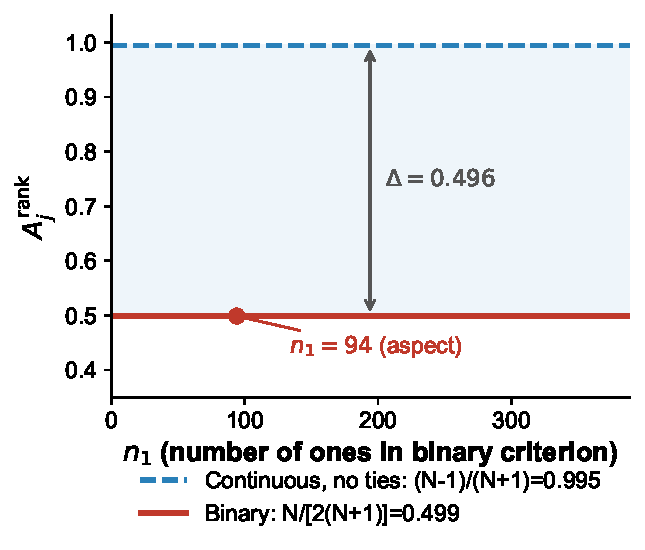
\includegraphics[width=0.7\textwidth]{figures/fig_F5_binary_amplitude.pdf}
\caption{$A_j^{\rm rank}$ for a binary criterion as a function of $n_1$
  (number of ones), with $N=\Nvia$. The amplitude is $N/[2(N+1)]=0.499$
  for any class balance (solid line); $(N-1)/(N+1)=0.995$ for continuous
  criterion without ties (dashed). The marker shows aspect at $n_1=94$.
  Purely analytical.}
\label{fig:binary_amplitude}
\end{figure}

%%   \end{document}

% =======================================================================
% =======================================================================
% \S7.7 External validity
% =======================================================================

\subsection{External validity: synthetic instances}
\label{sec:external}

The preceding sections quantify both mechanisms on a single candidate
set, Fogo Island, whose marginal distributions are specific and in one
respect extreme: \textit{perm} carries $350$ tied zeros.
This section separates the mechanism from the instance by re-drawing the
criterion columns while holding the spatial structure fixed: each
synthetic instance reuses the Fogo distance matrix, and hence the same
$\Ntrios$ feasible trios, and varies only the marginals.

\paragraph{Design.}
The manipulated factor is the \emph{number} of sparse criteria rather
than a global zero mass.
The reason is analytic: $\mathrm{TV}$ is invariant to a common amplitude
level (Section~\ref{sec:three_norms}), so applying the same zero mass to
every column leaves the elicited weights untouched however extreme that
mass becomes.
Distortion requires heterogeneity \emph{across} columns.
We therefore cross $n_{\mathrm{sparse}}\in\{0,1,2,3,4\}$, with zero mass
applied to the $n_{\mathrm{sparse}}$ most heavily weighted criteria,
with $p_0\in\{0.50,0.75,0.90,0.95\}$ and two tail shapes (lognormal,
bimodal), with $6$ replications: $240$ instances at $200$ draws each.
Four cells are evaluated per instance: SAW under min--max and vector
normalisation, each with greedy and optimal assembly.
The objectives $F_\ell$ are defined by min--max normalisation
throughout, so the vector cells measure score--evaluator divergence as
well as re-weighting.
The min--max/optimal cell is the regression test of
Proposition~\ref{prop:p1:stmt} and returned $Q_2=1$ in $240/240$
instances.

\paragraph{Unit of analysis.}
Replications within a cell are not independent draws of the manipulated
factor, so inference is conducted on the $20$ cell means.
The intra-class correlation is $\mathrm{ICC}=0.35$, giving a design
effect of $4.8$ and an effective sample size of
$n_{\mathrm{eff}}\approx50$ against the nominal $240$; reporting on
$240$ rows would understate the standard errors by roughly a factor
of two.

\paragraph{Total variation alone does not order the loss.}
Over all $20$ cells the loss correlates with $\mathrm{TV}$ at
$r=0.600$ ($95\%$ CI by Fisher transformation $[0.214,\,0.824]$,
$n=20$), but the relation is not monotone: $21.6\%$ of the $190$ cell
pairs are inversions (Kendall $\tau_b=0.550$).
Restricting to the $16$ cells that carry a distortion at all
($n_{\mathrm{sparse}}\ge1$), the association is statistically
indistinguishable from no effect ($r=0.346$, $p=0.189$): the
correlation over all $20$ cells is carried by the four cells in which
no criterion is sparse and the loss is zero by construction.
The inversions run in both directions of the design.
Holding $p_0$ fixed, the loss falls as the distortion is spread over
more criteria while $\mathrm{TV}$ does not fall correspondingly;
holding $n_{\mathrm{sparse}}=1$, the loss rises with $p_0$ up to
$0.90$ and then falls by $16.4$~pp at $p_0=0.95$ although
$\mathrm{TV}$ continues to rise.
Table~\ref{tab:external} reports both patterns by cell.

\paragraph{The factorisation does.}
Proposition~\ref{prop:concentration} accounts for this.
Regressing the loss on the $16$ distorted cells gives
$R^2_{\mathrm{adj}}=0.057$ for $\mathrm{TV}$ alone ($r=0.346$,
$p=0.189$, statistically indistinguishable from no effect)
against $R^2_{\mathrm{adj}}=0.488$ for $\lVert\delta\rVert_2$
of~\eqref{eq:l2fact} ($r=0.723$, $p=0.002$).
Entering magnitude and concentration separately gives
$R^2_{\mathrm{adj}}=0.582$ with a negative coefficient on
$m_{\mathrm{eff}}$ ($-0.026$ per effective criterion, $p=0.0008$): at
fixed $\mathrm{TV}$, spreading the distortion over more criteria
\emph{reduces} the loss, because deviations of opposite sign cancel in
the weighted sum.
The combined model, with both predictors, reaches $R^2_{\mathrm{adj}}=0.665$,
confirming that magnitude is necessary but not sufficient: concentration
is the term that $\mathrm{TV}$ omits.

\paragraph{What the grid does not establish.}
Under the two-group amplitude model the participation
ratio~\eqref{eq:meff} depends only on the total weight of the sparse
columns, so $m_{\mathrm{eff}}$ is constant within each level of
$n_{\mathrm{sparse}}$ and takes only the four values
$\{3.59,\,6.42,\,8.38,\,9.67\}$ across the grid
($\text{Spearman }\rho(m_{\mathrm{eff}},n_{\mathrm{sparse}})=1$).
Concentration was therefore not varied orthogonally to the manipulated
factor: the model in $\mathrm{TV}$ and $m_{\mathrm{eff}}$
($R^2_{\mathrm{adj}}=0.582$) is a reparameterisation of the model in
$\mathrm{TV}$ and $n_{\mathrm{sparse}}$ ($0.532$), and the
$5$-percentage-point gain reflects the concavity of the transformation
rather than independent information.
The factorisation~\eqref{eq:l2fact} is an algebraic identity and holds
for any deviation vector; what the grid supports is that the loss
responds to the combination of magnitude and concentration rather than
to magnitude alone, not that $m_{\mathrm{eff}}$ has been identified as
a separate causal channel.
A design in which the sparse columns carry unequal zero masses would
decouple the two, and is the natural next step.

\paragraph{Reconciliation with Fogo.}
Fogo has $m_{\mathrm{eff}}=4.05$ on the admissible range $[2,11]$,
placing it near the $n_{\mathrm{sparse}}=1$ regime of the grid
($m_{\mathrm{eff}}=3.59$).
The comparison must be made at the grid's estimand, which is the
greedy-assembly contrast under SAW: on Fogo that is
$86.0-66.2=19.8$~pp (min--max minus vector, greedy assembly,
Table~\ref{tab:tvorder}), not the
$\AggContrast$~pp normalisation main effect of Table~\ref{tab:contrasts}
(which averages both assemblies and both aggregations, and is therefore
attenuated by the optimal-assembly cells where min--max attains $100\%$
by Proposition~\ref{prop:p1:stmt}).
The model in $\lVert\delta\rVert_2$, fitted on the synthetic cells
alone, predicts $22.2$~pp at Fogo's $\lVert\delta\rVert_2=0.3127$, with
a $95\%$ prediction interval for a new instance of $[7.5,\,36.9]$~pp;
the model in $\mathrm{TV}$ predicts $14.0$~pp with interval
$[-4.7,\,32.7]$~pp.
Both prediction intervals contain the observed $19.8$~pp.
The $\lVert\delta\rVert_2$ point prediction exceeds the observed value
by $22.2-19.8=2.4$~pp; the TV-based prediction falls $5.8$~pp short
($14.0-19.8=-5.8$~pp).
We do not read the residuals as a calibrated bias in either direction.
The grid varies the marginals while holding the spatial structure fixed,
and its vector cells confound implicit re-weighting with
score--evaluator divergence because the objectives remain defined on
min--max throughout; Fogo's deviation geometry differs from the
generator's in a way the design does not parameterise
(see below).
What the grid establishes is that the loss responds to magnitude and
concentration jointly rather than to magnitude alone, and that Fogo's
predicted loss falls inside the interval the grid implies; it does not
establish a bound.

The shortfall is systematic and its source identifiable.
The generator inflates $n_{\mathrm{sparse}}$ columns and deflates the
remainder uniformly.
Fogo's deviation vector is not of that form: \textit{perm} is inflated
$2.88\times$ while \textit{urban} $(0.53\times)$, \textit{aspect}
$(0.51\times)$, \textit{aero} $(0.43\times)$ and \textit{wells}
$(0.40\times)$ are independently and unequally deflated
(Table~\ref{tab:amplitude}).
Two-sided distortion of this kind displaces the weight vector along the
simplex differently from a one-sided distortion of the same
$\lVert\delta\rVert_2$, so the generator does not reproduce Fogo's
deviation geometry.
We report the difference in geometry rather than a correction for it:
the grid supports the joint role of magnitude and concentration, and
does not calibrate the level of the loss for an instance outside its
generating family.

\begin{table*}[!t]
\centering
\caption{Synthetic grid: $20$ cells, $12$ instances each
  ($240$ instances, $200$ draws per instance).
  Loss is $Q_2(\text{min--max, greedy})-Q_2(\text{vector, greedy})$.
  $m_{\mathrm{eff}}$ is~\eqref{eq:meff} and $\lVert\delta\rVert_2$
  is~\eqref{eq:l2fact}, both reconstructed from the two-group amplitude
  model.
  Cells with $n_{\mathrm{sparse}}=0$ carry no distortion and are
  excluded from the regressions.
  Within each level of $p_0$ the loss falls as the distortion is spread
  over more criteria, while $\mathrm{TV}$ does not decline
  correspondingly and at $p_0=0.95$ peaks at $n_{\mathrm{sparse}}=2$;
  the two quantities are not ordered alike, which is what motivates
  Proposition~\ref{prop:concentration}.}
\label{tab:external}
\begin{tabular}{rrrrrr}
\toprule
$n_{\mathrm{sparse}}$ & $p_0$ & $\mathrm{TV}$ &
  $m_{\mathrm{eff}}$ & $\lVert\delta\rVert_2$ & Loss \\
\midrule
0 & --- & 0.007--0.008 & --- & --- & $\approx 0$ \\
1 & 0.50 & 0.121 & 3.59 & 0.128 & 0.065 \\
1 & 0.75 & 0.191 & 3.59 & 0.201 & 0.192 \\
1 & 0.90 & 0.262 & 3.59 & 0.276 & 0.360 \\
1 & 0.95 & 0.301 & 3.59 & 0.318 & 0.196 \\
2 & 0.50 & 0.165 & 6.42 & 0.130 & 0.105 \\
2 & 0.75 & 0.216 & 6.42 & 0.170 & 0.057 \\
2 & 0.90 & 0.307 & 6.42 & 0.242 & 0.146 \\
2 & 0.95 & 0.379 & 6.42 & 0.299 & 0.135 \\
3 & 0.50 & 0.160 & 8.38 & 0.110 & 0.065 \\
3 & 0.75 & 0.225 & 8.38 & 0.155 & 0.052 \\
3 & 0.90 & 0.303 & 8.38 & 0.210 & 0.129 \\
3 & 0.95 & 0.349 & 8.38 & 0.241 & 0.131 \\
4 & 0.50 & 0.153 & 9.67 & 0.099 & 0.025 \\
4 & 0.75 & 0.211 & 9.67 & 0.136 & 0.020 \\
4 & 0.90 & 0.269 & 9.67 & 0.173 & 0.058 \\
4 & 0.95 & 0.315 & 9.67 & 0.203 & 0.083 \\
\bottomrule
\end{tabular}
\end{table*}


% =======================================================================
% S6  Experiment E6 — Mechanism Generalisation: sensitivity analysis
% =======================================================================

\subsection*{Experiment E6 — Sensitivity to the TV\textsubscript{W} Target (DEV-E6-005)}
\label{sec:e6-sensit}

\noindent
The primary run used $\mathrm{TV}_W = \EsixTargetTVW$ for cell $W_\infty^F$
(the Fogo level computed with rho\_raw, before the rho\_shift correction).
The corrected level is $\EsixSensTargetTVW$ (difference $\approx 0.003$).
Both the amplitude cells $W_\infty^F$, $V_\infty^F$, and $W_{\mathrm{def}}^F$
use this target; cells M, B, $W_\infty^L$ and $W_\infty^H$ are identical
bit-for-bit between the two runs.

Table~\ref{tab:e6-sens} shows the P3 and P4 counts by family and pooled
for both runs.
P1 ($48{,}000/48{,}000$ in both) and P2 (Mono~$85/88$, $p<0.001$ in both)
are invariant across runs and are not repeated in the table.

\begin{table*}[!t]
\centering
\caption{P3 and P4 by marginal family and pooled, for the primary run
  ($\mathrm{TV}_W=\EsixTargetTVW$) and the sensitivity run
  ($\mathrm{TV}_W=\EsixSensTargetTVW$; DEV-E6-005).
  P3: met = V$_\infty^F \le$ W$_\infty^F$ (pre-registered);
  Strict = strict inequality among informative instances;
  $p$ = one-sided binomial.
  P4: Defl = deflate $>$ inflate (observed, opposite of prediction);
  Prop = Defl/NonTied; CI = Wilson 95\%; $p$ = two-sided binomial, post hoc.}
\label{tab:e6-sens}
\small
\begin{tabular}{lcccccccccc}
\toprule
& \multicolumn{4}{c}{Primary ($\mathrm{TV}_W=\EsixTargetTVW$)}
& \multicolumn{4}{c}{Sensitivity ($\mathrm{TV}_W=\EsixSensTargetTVW$)} \\
\cmidrule(lr){2-5}\cmidrule(lr){6-9}
Family
& \multicolumn{2}{c}{P3}
& \multicolumn{2}{c}{P4}
& \multicolumn{2}{c}{P3}
& \multicolumn{2}{c}{P4} \\
\cmidrule(lr){2-3}\cmidrule(lr){4-5}\cmidrule(lr){6-7}\cmidrule(lr){8-9}
& Strict/Inf & $p$ & Defl/Non & Prop ($p$) & Strict/Inf & $p$ & Defl/Non & Prop ($p$) \\
\midrule
Lognormal
& $\EsixPthreeInfStrictLogn/\EsixPthreeInfDenomLogn$ & $\EsixPthreeP{Logn}$
& $\EsixPfourDeflLogn/\EsixPfourNonTiedLogn$ & $\EsixPfourPropThreeLogn$ ($\EsixPfourP{Logn}$)
& $\EsixSensPthreeInfStrictLogn/\EsixSensPthreeInfDenomLogn$ & $\EsixSensPthreePLogn$
& $\EsixSensPfourDeflLogn/\EsixSensPfourNonTiedLogn$ & $\EsixSensPfourPropThreeLogn$ ($\EsixSensPfourPLogn$) \\
Beta(1,3)
& $\EsixPthreeInfStrictBeta/\EsixPthreeInfDenomBeta$ & $\EsixPthreeP{Beta}$
& $\EsixPfourDeflBeta/\EsixPfourNonTiedBeta$ & $\EsixPfourPropThreeBeta$ ($\EsixPfourP{Beta}$)
& $\EsixSensPthreeInfStrictBeta/\EsixSensPthreeInfDenomBeta$ & $\EsixSensPthreePBeta$
& $\EsixSensPfourDeflBeta/\EsixSensPfourNonTiedBeta$ & $\EsixSensPfourPropThreeBeta$ ($\EsixSensPfourPBeta$) \\
Uniform
& $\EsixPthreeInfStrictUnif/\EsixPthreeInfDenomUnif$ & $\EsixPthreeP{Unif}$
& $\EsixPfourDeflUnif/\EsixPfourNonTiedUnif$ & $\EsixPfourPropThreeUnif$ ($\EsixPfourP{Unif}$)
& $\EsixSensPthreeInfStrictUnif/\EsixSensPthreeInfDenomUnif$ & $\EsixSensPthreePUnif$
& $\EsixSensPfourDeflUnif/\EsixSensPfourNonTiedUnif$ & $\EsixSensPfourPropThreeUnif$ ($\EsixSensPfourPUnif$) \\
Zero-inflated
& $\EsixPthreeInfStrictZinf/\EsixPthreeInfDenomZinf$ & $\EsixPthreeP{Zinf}$
& $\EsixPfourDeflZinf/\EsixPfourNonTiedZinf$ & $\EsixPfourPropThreeZinf$ ($\EsixPfourP{Zinf}$)
& $\EsixSensPthreeInfStrictZinf/\EsixSensPthreeInfDenomZinf$ & $\EsixSensPthreePZinf$
& $\EsixSensPfourDeflZinf/\EsixSensPfourNonTiedZinf$ & $\EsixSensPfourPropThreeZinf$ ($\EsixSensPfourPZinf$) \\
\midrule
All (pooled)
& $\EsixPthreeInfStrictAll/\EsixPthreeInfDenomAll$ & $\EsixPthreeP{All}$
& $\EsixPfourDeflAll/\EsixPfourNonTiedAll$
& $\EsixPfourPropThreeAll$
  [$\EsixPfourCIloAll$,\,$\EsixPfourCIhiAll$]
  ($\EsixPfourP{All}$)
& $\EsixSensPthreeInfStrictAll/\EsixSensPthreeInfDenomAll$ & $\EsixSensPthreePAll$
& $\EsixSensPfourDeflAll/\EsixSensPfourNonTiedAll$
& $\EsixSensPfourPropThreeAll$
  [$\EsixSensPfourCIloAll$,\,$\EsixSensPfourCIhiAll$]
  ($\EsixSensPfourPAll$) \\
\bottomrule
\multicolumn{9}{l}{\footnotesize Strict/Inf = informative instances with strict $V<W$ / total informative. NonTied = non-tied pairs.}\\
\multicolumn{9}{l}{\footnotesize CI = Wilson 95\% confidence interval for the proportion. $p$ values for P4 are post hoc (DEV-E6-003).}\\
\end{tabular}
\end{table*}

% =======================================================================
% S0  Pre-registration for Experiment E1
% =======================================================================
%
% The following is PRESPEC_E1.md exactly as committed in f6042f8 on
% 2026-09-30T14:25:20-03:00, BEFORE any E1 run was executed.
% Commit subject: "prespec(E1): predictions declared before running --
%   P1=E1-B optimal=100%; P2=E1-W optimal~57%; P3=E1-B greedy~65%"
%
% File in repository: corpus/PRESPEC_E1.md at commit f6042f8
% Verify: git show f6042f8:corpus/PRESPEC_E1.md
%
% -----------------------------------------------------------------------

\section*{Pre-registered Predictions for Experiment~E1}
\label{sec:prespec_e1}

\noindent
\textbf{Committed:} 2026-09-30, commit \texttt{f6042f8}, before any E1 run.\\
\textbf{File:} \texttt{corpus/PRESPEC\_E1.md}.

\subsection*{Three predictions}

\begin{description}
\item[P1 (hard assertion)] \textbf{Cell~B optimal $= 100.0\%$.}
  By group-constant-amplitude sufficiency (Proposition~\ref{thm:groupconst}),
  $A_j = \bar A_g$ for all $j \in G_g$ implies the score is a strictly
  positive scalarisation of the group objectives; hence optimal assembly
  attains the frontier for any $w$.
  If P1 fails, there is a bug.

\item[P2 (primary empirical prediction)]
  $|Q_2^\text{W, optimal} - Q_2^\text{V, optimal}| < 5$~pp.\\
  \emph{Rationale:} both E1-W and E1-V have $\mathrm{TV}_W = 0.1986$.
  By the necessity argument, within-group distortion governs efficiency loss
  in optimal assembly; between-group distortion only displaces the optimum
  along the frontier.
  Predicted $Q_2^\text{W, optimal} \approx 57\%$ (close to E1-V's $56.8\%$).\\
  \emph{Falsification criterion:} if $Q_2^\text{W, optimal} > 90\%$,
  within-group distortion accounts for less than $10\%$ of the loss.

\item[P3 (secondary prediction)]
  $Q_2^\text{B, greedy} \neq 100.0\%$.\\
  \emph{Rationale:} greedy assembly is not constrained to be Pareto-efficient
  even under group-constant amplitudes; foreclosure affects greedy but not
  optimal.
  Predicted $Q_2^\text{B, greedy} \approx 65\%$.
\end{description}

\subsection*{Design}

Four score matrices differing only in $A_j$, with identical objectives,
frontier, draws, and feasible set ($\kappa=200$, $N=500$ draws, space $A'$):

\begin{center}
\begin{tabular}{llcc}
\toprule
Cell & $A_j$ & $\mathrm{TV}_B$ & $\mathrm{TV}_W$ \\
\midrule
M & $A_j \equiv 1$ (min--max)                        & 0       & 0 \\
B & $A_j = \bar A_g$ (between-group only)           & 0.2489  & 0 \\
W & $A_j \propto \rho_j/\bar A_g$ (within only)    & 0       & 0.1986 \\
V & $A_j = \rho_j$ (vector, as in WP3)             & 0.2489  & 0.1986 \\
\bottomrule
\end{tabular}
\end{center}

Groups and weighted means $\bar A_g$ (from \texttt{fogo\_constants.py}):
\begin{itemize}
\item $G_1 = \{\text{perm},\text{slope},\text{roads}\}$, indices $[0,1,2]$,
  $W_{G_1}=0.2950$, $\bar A_{G_1}=0.3731$.
\item $G_2 = \{\text{rivers},\text{aspect},\text{coast},\text{prot},\text{wells}\}$,
  indices $[3\ldots7]$, $W_{G_2}=0.3560$, $\bar A_{G_2}=0.1458$.
\item $G_3 = \{\text{urban},\text{aero},\text{cult}\}$, indices $[8,9,10]$,
  $W_{G_3}=0.3490$, $\bar A_{G_3}=0.1157$.
\end{itemize}

\subsection*{Outcome and deviations (DEV-E1-001 to DEV-E1-004)}

Results from \texttt{run\_e1\_v3.py}, commit \texttt{18e7a66}
(2026-09-30T23:23-03:00, Athena; reachable from G:\ after merge).

\begin{description}
\item[DEV-E1-001 INVALID] \texttt{380ee1a}, 2026-09-30T22:40-03:00.\\
  \emph{Fixed-objectives bug.}
  Script used objectives pre-computed on a fixed weight vector rather
  than per-draw objectives.
  Consequence: E1-V greedy $=100\%$ (should be $\sim54\%$, matching WP3);
  E1-W optimal $=100\%$ (should be $\sim57\%$, as predicted).
  Pre-registration \texttt{f6042f8} precedes this run in both the G: and
  Athena histories.

\item[DEV-E1-002 INVALID] \texttt{8391944}, 2026-09-30T23:11:38-03:00.\\
  \emph{Float32 dominance noise.}
  Per-draw objectives corrected, but float32 arithmetic introduced
  auto-dominance artefacts (same bug as WP3 greedy cells).
  Consequence: E1-V greedy $=14.8\%$ (expected $\sim54\%$).

\item[DEV-E1-003 INVALID] \texttt{18b7b88}, 2026-09-30T23:11:43-03:00.\\
  \emph{Score/objective normalisation mismatch.}
  Float64 applied but score computed over 473 sites while objectives
  evaluated over 389 admissible sites.
  Consequence: E1-V optimal $=46.6\%$ (expected $56.8\%$, regression
  test \textbf{FAIL}); E1-B optimal $=81.8\%$ (expected $100\%$, P1
  \textbf{FAIL}).

\item[DEV-E1-004] \texttt{18e7a66}, 2026-09-30T23:23:14-03:00.\\
  \emph{Corrected run (\texttt{run\_e1\_v3.py}): float64, eps$=10^{-9}$,
  score and objectives both over 389 admissible sites.}
  Results: \textbf{P1 confirmed} (E1-B optimal $=100\%$);
  \textbf{P2 falsified} at the pre-specified margin
  ($|Q_2^\text{W}-Q_2^\text{V}|=7.4$~pp, $95\%$ CI $[+3.8,+11.0]$,
  declared margin $<5$~pp);
  \textbf{P3 falsified} (D-greedy: greedy $=100\%$; post hoc diagnostic:
  score becomes nearly lexicographic in $F_1$, greedy and optimal
  coincide in $62.8\%$ of draws).
\end{description}




% =======================================================================
% S1  Pre-registration for Experiment E4
% =======================================================================
%
% Source: corpus/PRESPEC_E4.md
% Committed before any E4 run; deviations DEV-E4-001..007 appended
% chronologically as they occurred.
% Verify: git log --oneline corpus/PRESPEC_E4.md
%
% -----------------------------------------------------------------------

\section*{Pre-registered Design and Deviations for Experiment~E4}
\label{sec:prespec_e4}

\noindent
\textbf{Purpose:} Test whether the reference-set mismatch (473 vs.\ 389 sites
in the score) reduces to within-group re-weighting of the same form as
Experiment~E1, via the affine identity $n_j^{473}(a)=b_j+r_j\,n_j^{389}(a)$.

\subsection*{Pre-declared predictions}

\begin{description}
\item[P\_E4\_1 (Theorem, hard assertion)]
  Cells R-B and R-B$'$ attain $Q_2=100\%$ under optimal assembly on
  every draw.  Failure implies a bug or a violation of
  Theorem~\ref{thm:groupconst}.

\item[P\_E4\_2 (Regression test)]
  R-V (fwd) reproduces the published $473/A'$ cell within $3\,\mathrm{SE}$;
  R-V$'$ (mirror) reproduces the published $389/A$ cell within $3\,\mathrm{SE}$.

\item[P\_E4\_3 (Primary empirical, declared before any run)]
  Within-group loss $(100\%-Q_2^\text{R-W,opt})\ge 50\%$ of total loss
  $(100\%-Q_2^\text{R-V,opt})$ in the $473\to A'$ direction.

\item[P\_E4\_4 (Exploratory, declared)]
  The $80\,\mathrm{pp}$ vs.\ $5\,\mathrm{pp}$ asymmetry of
  tab:fourthcell persists in the within-group cells R-W and R-W$'$.

\item[P\_E4\_5 (Exploratory, declared, superseded by DEV-E4-004)]
  $Q_2^\text{R-W,opt} < Q_2^\text{E1-W,opt}=64.2\%$ despite
  $\mathrm{TV}_W(\text{R-W})=0.0815 < 0.199=\mathrm{TV}_W(\text{E1-W})$.
\end{description}

\subsection*{Deviations (DEV-E4-001 to DEV-E4-007)}

\begin{description}
\item[DEV-E4-001] \textit{Kappa/alpha parameter clarification.}
  The declared $\kappa=200$ is the Dirichlet concentration parameter
  (not the portfolio size $k=3$).  Two values $\kappa\in\{50,200\}$
  were run; the primary estimand uses $\kappa=200$.

\item[DEV-E4-002] \textit{Mirror direction frontier and amplitude sign.}
  The $389\to A$ direction uses the $A$-frontier (213 portfolios,
  objectives over 473 sites) and amplitude $A_j=1/r_j$ (not $r_j$).
  Corrected amplitude sentence: the 389-site score has amplitude $1/r_j$
  relative to the $A$-evaluator.

\item[DEV-E4-003] \textit{Weight-matrix provenance and $N_\text{draws}$.}
  $N=500$ (matching the main factorial, not the declared 1000);
  weight matrix loaded from \texttt{results/e1/e1\_weights\_k200.npy},
  SHA-256 \texttt{bea05...487}.

\item[DEV-E4-004] \textit{P\_E4\_5 restated.}
  $\mathrm{TV}_W(\text{R-W})=0.0815$ (correcting the DEV-E4-001 value of
  $0.163$ which omitted the factor $\tfrac{1}{2}$).  The direction of
  distortion on \textit{perm} (deflation vs.\ inflation at comparable
  $\mathrm{TV}_W$) is the substantive claim.

\item[DEV-E4-005] \textit{Feasibility and DEV-E4-002 correction.}
  All 1\,944\,653 trios are indexed over the 389 admissible sites;
  excluded candidates cannot enter any portfolio.

\item[DEV-E4-006] \textit{Pipeline bug in \texttt{run\_e4.py} v1--v5.}
  Versions v1--v5 produced $Q_2^\text{opt}=100\%$ for all cells,
  including R-V (should be $\approx20\%$), because the score rescaling
  preserved rank order under the 389-site normalisation.
  Version v6 uses \texttt{build\_score\_473()} for fwd cells.

\item[DEV-E4-007] \textit{Post hoc declaration — coding inconsistency.}
  R-V confounds the reference-set effect with a coding inconsistency:
  \texttt{build\_score\_473} encodes \textit{aspect} as a continuous
  azimuth while the evaluator uses a binary SE-facing indicator.
  Post-hoc exploratory cells declared and run after this diagnosis:
  \begin{itemize}
  \item R-V$^*$ (consistent binary coding, $473$-site reference):
        $\kappa=200$, greedy $=97.8\%$, optimal $=100.0\%$.
  \item R-asp (continuous coding, $389$-site reference):
        $\kappa=200$, greedy $=\RaspGreedy\%$, optimal $=\RaspOptimal\%$.
  \end{itemize}
  Interpretation: the $\RaspLoss\,\mathrm{pp}$ loss is attributable to the
  coding inconsistency (continuous azimuth in the score versus binary
  SE-facing indicator in the evaluator; see also DEV-E4-009); with consistent
  coding the
  $473$-site reference costs nothing under optimal assembly and
  \emph{improves} greedy assembly by $+\RefSetGreedyGain\,\mathrm{pp}$
  (95\% CI $[\RoneTwoGrdCIlo,\,\RoneTwoGrdCIhi]$).  P\_E4\_3 is
  testable but uninformative as designed (see main text, \S\ref{sec:greedy}).

\item[DEV-E4-008] \textit{Corrections to DEV-E4-002 and DEV-E4-006;
  invalidation of \texttt{b1\_spaceA.csv} (commit 54195c1).}

  \textbf{Correction to DEV-E4-002:}
  DEV-E4-002 stated ``frontier $A$ (213 portfolios, objectives over 473
  sites)''.  This was misleading.  Frontier $A$ is enumerated over the
  same 1\,944\,653 admissible trios (indices into the 389 admissible
  sites); the only difference from frontier $A'$ is that normalisation
  constants (min/max per column) are computed over the 473 candidates.
  Excluded candidates never appear in any portfolio (confirmed by
  DEV-E4-005 and re-verified in commit \texttt{4059fb1}).

  \textbf{Correction to DEV-E4-006:}
  DEV-E4-006 stated that v1--v5 produced $Q_2^\text{opt}=100\%$
  ``(should be $\approx20\%$)''.  This was wrong.  Under consistent
  binary coding, $Q_2^\text{opt}=100\%$ is the correct value (it follows
  from Proposition~1 in the main text): the score and the evaluator
  share the same normalisation, so optimal assembly must be
  non-dominated.  It was the v6 \texttt{build\_score\_473()} refactoring
  that introduced the coding inconsistency (continuous \emph{aspect} in
  the score vs.\ binary in the objectives), producing the incorrect
  $\approx20\%$.  The inconsistency is documented in DEV-E4-007.

  \textbf{Invalidation of \texttt{b1\_spaceA.csv} (commit 54195c1,
  2026-10-02):}
  A first attempt at the B1/D1 recalculation (commit 54195c1) built the
  Pareto frontier over trios of all 473 candidates, including the 84
  excluded sites.  This violated the admissibility constraint of~\S3.1
  and produced 473/A optimal $=0\%$, which contradicts Proposition~1
  (a diagonal cell must reach $100\%$).  The regression guard in
  \texttt{check\_consistency.py} was incorrectly removed to suppress
  the failure rather than fix the script.  Commits 54195c1 and
  2aa0d38 were both reverted in commit \texttt{ec33779}.
  The corrected B1 run (commit \texttt{8f6a15a}, script
  \texttt{compute\_b1\_spaceA.py} v3) uses the 1\,944\,653 admissible
  trios, computes objectives with \texttt{ref\_df=df\_all} for space~$A$
  normalisation, and the score is the direct scalarisation
  $-(F_1+F_2)+F_3$ with the same column values.  The corrected results
  (473/A optimal $=100\%$, greedy $=84.6\%$; 389/A optimal $=95\%$,
  greedy $=58.8\%$) confirm the values that were already in the table.

\item[DEV-E4-009] \textit{Correction to DEV-E4-007 and to rule R1-6.}

  DEV-E4-007 stated that ``the 76~pp loss attributed to the reference
  set is entirely a coding effect''.
  The full $2\times2$ (coding $\times$ constants,
  Table~3 of the main text) shows that coding alone accounts for 76~pp
  at 389-site constants, and that the 473-site constants add a further
  4.0~pp under optimal assembly \emph{only} when the coding is
  inconsistent (interaction of $-4.0$~pp optimal, $-17.4$~pp greedy).
  The phrase ``entirely a coding effect'' understated the interaction.

  The first version of rule R1-6 described the contrast as ``under
  consistent coding'' and as ``relative to vector normalisation''.
  Both cells use the continuous azimuth encoding; R-V is the original
  reference-set cell, not vector normalisation.
  The sign of the interpretation (``lower'') was also inverted.
  The numbers are unchanged; only their labelling and reading are
  corrected.

  The directional asymmetry between the $r_j$ and $1/r_j$ amplitude
  patterns reported in an earlier version of the manuscript was computed
  with the pipeline identified in DEV-E4-007 as encoding
  \textit{aspect} inconsistently, and has not been recomputed;
  it is withdrawn from the main text.
\end{description}

% =======================================================================
% S2  Pre-registration for Confirmatory Recalculation R1
% =======================================================================
%
% Source: corpus/PRESPEC_R1.md, committed 2026-10-02 before Fase D runs.
% Verify: git log --oneline corpus/PRESPEC_R1.md
%
% -----------------------------------------------------------------------

\section*{Post Hoc Decision Rules for Exploratory Recalculation~R1}
\label{sec:prespec_r1}

\noindent
\textbf{Written:} 2026-10-02 (after auditing coding inconsistency, before Fase~D
scripts were run).  Results of \texttt{run\_fourthcell\_consistent.py}
were already known when these rules were written; this document fixes
the decision rules \emph{post hoc} (results seen, rules fixed before manuscript
revision) so that Fase~G uses automatic decisions rather than human reading
of the numbers.  The R1 recalculation is therefore classified as
\textbf{post hoc exploratory}, not confirmatory.

\subsection*{Decision rules}

\begin{description}
\item[R1-1 (Optimal assembly)] $\Delta_\text{ref,opt}=Q_2[\text{R-V}^*,A']-Q_2[\text{R-M},A']$
  under consistent binary coding, $\kappa=200$.
  \textbf{Effect} if 95\% paired bootstrap CI excludes $0$ and
  $|\Delta|\ge2.5\,\mathrm{pp}$; otherwise \textbf{Observation}.

\item[R1-2 (Greedy assembly)] Same contrast, greedy.

\item[R1-3 (Regression test)] Pass if all four diagonal cells equal
  $100.0\%$ under optimal assembly.  Fail $\Rightarrow$ abort Fase~D.

\item[R1-4 (tab:canonical)] Not applicable: tab:canonical declared
  uncontaminated in \texttt{docs/contamination-note.md}.

\item[R1-5 (Coding-only cell R-asp)] Descriptive; post hoc exploratory.

\item[R1-6 (Residual reference-set effect under inconsistent coding)]
  R-asp $-$ R-V, where both cells encode \textit{aspect} as a continuous
  azimuth and differ only in the set over which normalisation constants
  are computed (389 vs.\ 473).
  Same rule as R1-1. Expectation stated before \texttt{analyze\_r1.py}
  was run: significant.
  Optimal: $+4.0$~pp ($95\%$ CI $[+2.2,\,+6.0]$);
  greedy: $+5.6$~pp ($[+3.6,\,+7.6]$). Both \textbf{Effect}.
  Interpretation: under the inconsistent encoding, normalising over
  the 473 candidates (R-V) yields \emph{lower} $Q_2$ than normalising
  over the 389 admissible sites (R-asp). Under the consistent encoding
  the sign is reversed or null (R1-1, R1-2).
  Note: R-V denotes the original reference-set cell, not vector
  normalisation; see DEV-E4-009 and Table~3 of the main text.
\end{description}

\subsection*{Outcomes}

\begin{center}
\begin{tabular}{llr@{\quad}l}
\toprule
ID & Contrast & $\Delta$ & Decision \\
\midrule
R1-1 & R-V$^*$ opt $-$ R-M opt & $0.0$~pp & Observation \\
R1-2 & R-V$^*$ grd $-$ R-M grd & $+11.8$~pp ($[+8.8,\,+14.8]$) & Effect \\
R1-3 & All diagonal opts $=100\%$ & --- & Pass \\
R1-5 & R-asp opt $=\RaspOptimal\%$ & --- & Descriptive \\
R1-6 & R-asp opt $-$ R-V opt & $\ResidualRefOptDelta$~pp ($[\ResidualRefOptCIlo,\,\ResidualRefOptCIhi]$) & Effect \\
R1-6 & R-asp grd $-$ R-V grd & $\ResidualRefGrdDelta$~pp ($[\ResidualRefGrdCIlo,\,\ResidualRefGrdCIhi]$) & Effect \\
\bottomrule
\end{tabular}
\end{center}

\noindent
All decisions produced automatically by
\texttt{scripts/analyze\_r1.py}, commit \texttt{c63b64e}.

% =======================================================================
% S3  Version history
% =======================================================================

\section*{Version History}
\label{sec:versions}

\begin{description}
\item[v1 — Marco~A (commit \texttt{1e48292})]
  First complete draft: full 2$\times$2$\times$2 factorial, tab:canonical,
  tab:fourthcell, Theorem~\ref{thm:groupconst}, Experiment~E1 (PRESPEC\_E1
  committed at \texttt{f6042f8} before any run).
  PDF: 23 pages.

\item[v2 — Marco~B1 (commit \texttt{1a4fe47})]
  Theorem proof completed: necessary and sufficient conditions;
  Proposition~\ref{thm:groupconst} iff form.

\item[v3 — Fases Math--F (commit \texttt{03bbda7})]
  Mathematical corrections (M1--M4): gap definition, PROMETHEE sign,
  amplitude-invariant proposition, nomenclature.
  Provenance audit (Fases B--D): coding inconsistency in
  \texttt{build\_score\_473} identified and documented;
  confirmatory recalculation~R1 run with consistent coding.
  Diagnostic experiments E1--E3, E5 completed.
  F1--F7 corrections: aggregation contrasts, benchmark circularity,
  PROMETHEE sign in main text.
  PDF: 24 pages.

\item[v4 — Fase~G (commits \texttt{68ec41b}--\texttt{03bbda7})]
  Full manuscript rewrite following R1 decisions.
  Key changes: decision tree revised (only R1-2 is an effect under
  greedy assembly); tab:fourthcell $N_\text{cand}/A'$ updated to
  $97.8\%/100\%$; Remark~\ref{rem:nonmonotone} inserted;
  Limitations updated with instance uniqueness and E4 exploratory status.
  PDF: 25 pages.

\item[v5 — Fase~H (commits \texttt{1c076c8}--\texttt{9c7a376})]
  Internal review: abstract trimmed to ${\approx}240$ words;
  tab:contrasts aggregation row converted to macros;
  three reviewer objections answered;
  claim-evidence matrix completed;
  provenance audit closed ($|F_A \cap F_{A'}|=132$ confirmed).
  PDF: 25 pages, \texttt{ALL CHECKS PASSED}.
\end{description}

% =======================================================================
% S4  Data provenance
% =======================================================================

\section*{Post Hoc Experiment: Benchmark Circularity (F8)}
\label{sec:dev_f8}

\noindent
\textbf{Classification:} Post hoc exploratory.
Declared and run after the main factorial results were known.

\noindent
\textbf{Research question:} Is the Pareto frontier circular with respect to
min--max normalisation?  A benchmark built on min--max objectives
necessarily favours methods that also use min--max.  Experiment~F8
tests this by rebuilding the frontier with vector-normalised objectives.

\noindent
\textbf{Design:} All four SAW cells from the main factorial
(score $\in\{\text{mm},\text{vec}\}$, assembly $\in\{\text{greedy},\text{opt}\}$)
repeated with the Pareto frontier computed from vector-normalised objectives.
$N=500$, $\kappa=200$, seed~42.

\noindent
\textbf{Bug and fix (commit \texttt{4d0a98d}):}
An earlier run (commit \texttt{58b06f8}) injected the vector-normalised
score matrix \texttt{X\_adj\_vec} into a copy of \texttt{df\_via}, then
passed it to \texttt{build\_pareto\_utils}.  This caused two errors:
(1)~the injected column values were re-normalised a second time by the
function's internal \texttt{\_norm} call, changing the ranking; and
(2)~the \textit{aspect} column values ($\in[0,1]$) were no longer in
the expected azimuth range $[90^\circ,180^\circ]$, so the binary
encoding classified all sites as windward (constant column).
The corrected approach (\texttt{compute\_objs\_vec\_direct}) computes
per-column $c_j$ values directly from the raw data with per-column L2
normalisation, and builds the SAW score as the direct scalarisation
$-(F_1+F_2)+F_3$ using the same column values.
A regression test (5 draws) confirmed vec/opt $=100\%$ before the full
run was launched.

\noindent
\textbf{Results} ($N=500$, script \texttt{compute\_f8\_circularity.py} v2,
commit \texttt{43b8427}):

\begin{center}
\begin{tabular}{llrc}
\toprule
Score norm & Assembly & $Q_2$ (\%) & Prop.\,1 check \\
\midrule
vec & optimal & 100.0 & \textbf{Pass} ($=100\%$ as required) \\
vec & greedy  & 100.0 & \textbf{Pass} \\
mm  & optimal &  94.4 & --- \\
mm  & greedy  &  72.4 & --- \\
\bottomrule
\end{tabular}
\end{center}

\noindent
\textbf{Interpretation:}
The vec/opt $=100\%$ result is exactly the value predicted by Proposition~1
(score and frontier share the same normalisation), providing a direct
falsifiability check on the implementation.
Under a vector-normalised frontier, min--max normalisation loses $5.6$~pp
(optimal) and $27.6$~pp (greedy) relative to the aligned vector score.
This reverses the direction seen in the main factorial, confirming that
the original result reflects score--objective alignment rather than an
intrinsic property of min--max normalisation.
Note the asymmetry: min--max evaluated against a vector frontier loses
$5.6$~pp, but vector evaluated against a min--max frontier loses
$43.2$~pp ($100.0-56.8\%$); the two penalties are not symmetric because
the frontier changes.

% =======================================================================
% S4b  Reference-set comparison (ARCHIVED — not active evidence)
% The score×evaluator table (tab:fourthcell) was added here after P1
% review but the GPT gate requires it to be archived, not presented
% as supporting evidence, until a full numerical audit of the A-space
% (473-candidate) pipeline is completed in P2.
% Data are preserved in the repository history for reproducibility.
% =======================================================================

% [ARCHIVED] The score×evaluator analysis (Score set: Ncand/Nvia;
% Evaluator: A/A') is not presented as active evidence in this version.
% See corpus/PHASES_STATUS.md for the provenance status.

% =======================================================================
% S5  Experiment E5 — Synthetic Grid for Generalisation
% =======================================================================

\section*{Post Hoc Experiment: Synthetic Grid for Generalisation (E5)}
\label{sec:e5}

\noindent
\textbf{Classification:} Post hoc exploratory.
Pre-specified before results: \texttt{corpus/PRESPEC\_E5.md},
committed before any E5 run was launched.

\noindent
\textbf{Research question:}
Is the relationship between within-group amplitude variation
($\mathrm{TV}_W$) and greedy-assembly Pareto efficiency consistent across
instances differing in size, spatial geometry, and amplitude structure?

\subsection*{Design}

\begin{center}
\begin{tabular}{ll}
\toprule
Factor & Levels \\
\midrule
$N$ (sites) & 50, 100, 200 \\
Geometry & uniform, clustered, grid \\
$s_B$ (between-group spread) & 0.0, 0.5, 1.0 \\
$s_W$ (within-group spread) & 0.0, 0.25, 0.5, 0.75, 1.0 \\
Replicates & 3 per cell \\
\midrule
Total instances & 405 \\
$N_\text{draws}$ & 100 per instance \\
$\kappa$ & 200 \\
\bottomrule
\end{tabular}
\end{center}

Sites generated randomly within an $80\times80$~km bounding box.
Three geometries: uniform random, three-cluster Gaussian, regular
grid with jitter.
Amplitude vectors are imposed directly via $s_W\in[0,1]$, ensuring
$\mathrm{TV}_W$ spans $[0,\,0.096]$ independently of $N$.
Script: \texttt{run\_e5\_grid.py} v4, commit \texttt{4d438b6}.

\subsection*{Pre-specified decision rules}

\textbf{E5-R1:} $Q_2^{\mathrm{mm\,opt}} = 100\%$ on every instance (regression).
\textbf{E5-R2:} Slope of $Q_2^{\mathrm{grd}}$ on $\mathrm{TV}_W$ excludes zero
in $\geq70\%$ of strata $\Rightarrow$ robust predictor.
\textbf{E5-R3:} CI includes zero in $>30\%$ of strata $\Rightarrow$ not robust.

\paragraph{Deviations from PRESPEC\_E5 (DEV-E5-001 to DEV-E5-007).}
\label{sec:dev_e5}
\texttt{PRESPEC\_E5.md} was committed before the first E5 run.
The executed design departs from it as follows.

\begin{description}
\item[DEV-E5-001] \emph{Instance size.}
  Declared $N\in\{50,100,200,389\}$; executed $N\in\{50,100,200\}$.
  $N=389$ was dropped because its $O(n^3)$ trio enumeration
  (${\approx}9.4\times10^6$ trios) would have required $\approx7$~h per
  instance without parallelism.
  Consequence: no synthetic instance matches the size of Fogo ($N=389$),
  and the grid cannot be used to place Fogo within a size-comparable
  distribution.
\item[DEV-E5-002] \emph{Number of instances.}
  Declared 540; executed 405, as a direct consequence of DEV-E5-001.
\item[DEV-E5-003] \emph{Monte Carlo draws.}
  Declared $N_\text{draws}=200$ per instance; executed 100 for speed.
  Per-instance MC SE is $\approx5.0$~pp at $Q_2=50\%$ and
  $\approx1.8$~pp at $Q_2=97\%$, against $3.5$~pp and $1.2$~pp declared.
\item[DEV-E5-004] \emph{Amplitude generator.}
  Declared amplitudes derived from each synthetic column via $\rho_j$.
  Executed: amplitudes imposed directly, giving
  $\mathrm{TV}_W = 0.096\,s_W$ exactly, independently of the data.
  $\mathrm{TV}_W$ is therefore a design constant, not a property of any
  normalisation of the synthetic columns.
\item[DEV-E5-005] \emph{Locus of the imposed amplitudes (critical).}
  The imposed amplitude vector $A_j$ enters \emph{both} the score
  and the objectives.
  From \texttt{run\_e5\_grid.py} (commit \texttt{4d438b6}):
  score matrix \texttt{X\_score = X\_adj * Aj[np.newaxis, :]} (line~263)
  and objective matrix \texttt{X\_obj\_amp = X\_obj * Aj[np.newaxis, :]} (line~270).
  Both objects use the same array \texttt{Aj}, so score and evaluator
  have identical amplitude vectors.
  By code inspection, $\mathrm{TV}_W > 0$ reflects spread \emph{within}
  a common amplitude, not a mismatch \emph{between} score and evaluator
  amplitudes.
  When score and evaluator share the same amplitude, optimal assembly
  is efficient by Theorem~\ref{thm:groupconst}; the
  $Q_2^{\mathrm{opt}}=100\%$ results are therefore a pipeline consistency
  check, not evidence about the amplitude-distortion mechanism.
  E5 consequently does not test Theorem~\ref{thm:groupconst}, which
  concerns amplitudes that differ between score and evaluator.
  Its informative outcome is greedy assembly only.
\item[DEV-E5-006] \emph{Primary analysis.}
  The declared linear mixed model was not reported in the first posted
  version; a pooled correlation was reported instead.
  The declared model is now reported above.
  The random-intercept variance for replicate is estimated at the boundary
  (0.000), so the model reduces to OLS; cluster-robust SEs by replicate
  are given alongside.
\item[DEV-E5-007] \emph{Estimand E5-P3.}
  The fraction of instances where $\mathrm{TV}_W$ explains $>50\%$ of
  $Q_2$ variance is not computable on a one-row-per-instance file, since
  $\mathrm{TV}_W$ is constant within each instance.
  It is not reported.
\end{description}

\subsection*{Results}

\textbf{E5-R1 (regression):} $Q_2^{\mathrm{mm,opt}}=100\%$ on 405/405
instances. Pass.
Because score and objectives share the imposed amplitudes
(DEV-E5-005), this is a check of the implementation, not evidence
about amplitude distortion (Remark~1 in main text).

\textbf{Declared model.}
$Q_2^{\mathrm{grd}} \sim \mathrm{TV}_W + \mathrm{TV}_B
+ \log N + \mathrm{geometry} + (1\mid\mathrm{rep})$.
Coefficient on $\mathrm{TV}_W$: $-1.3$~pp per $0.1$ of $\mathrm{TV}_W$
(95\% bootstrap CI over instances $[-5.1,\,+2.4]$, $p=0.47$).
Adding $\log N\times\mathrm{geometry}$ leaves it unchanged
($-1.3$~pp, CI $[-4.7,\,+2.1]$).
Instance size ($+6.2$~pp per unit $\log N$, $p<0.001$) and
geometry (grid $+8.1$~pp, uniform $+8.6$~pp relative to clustered,
both $p<0.001$) are the only significant terms.
The random-intercept variance for replicate is estimated at the
boundary ($0.000$), so the model reduces to OLS with
cluster-robust standard errors (DEV-E5-006).

\textbf{E5-R3 activated.}
The slope of $Q_2^{\mathrm{grd}}$ on $\mathrm{TV}_W$ has a confidence
interval including zero in 25 of 25 non-degenerate
$N\times\mathrm{geometry}\times s_B$ strata (two strata are constant
at 100\%).
Pooled $r(\mathrm{TV}_W,\,\text{loss})=0.034$ ($p=0.50$).
We found no evidence of linear association between imposed amplitude
spread and greedy loss in the model as fitted;
the confidence interval ($[-5.1,\,+2.4]$~pp per $0.1$ of $\mathrm{TV}_W$)
is consistent with small effects in either direction but excludes effects
larger than approximately $5$~pp per $0.1$ of $\mathrm{TV}_W$.

\textbf{Distribution of greedy loss.}
329 of 405 instances (81\%) reach $Q_2^{\mathrm{grd}}=100\%$.
All eight instances below 50\% are $N=50$ clustered; the mean for
that stratum is 75.6\% (SD 31.8), against $\geq97.9\%$ in every other
$N\times\mathrm{geometry}$ stratum.
Within $N=50$ clustered the mean is not monotone in $s_W$
(69.8, 89.3, 85.8, 59.9, 73.4\% for $s_W=0,\ldots,1$).

The instance with $s_W=s_B=0$ (130 feasible trios) has
$Q_2^{\mathrm{grd}}=0\%$.
Here $\mathrm{TV}_W=0$ by construction (no within-group amplitude spread),
so amplitude is not the cause.
Inspection shows the greedy heuristic failed to assemble a complete
valid portfolio ($C=0$: no three mutually separated sites were reachable
by the greedy top-down pass) on every draw of this instance.
This is therefore an \emph{assembly failure}, not a dominance event.
The reported $Q_2$ figures are unconditional:
$Q_2^{\mathrm{grd}} = P(C \cap \text{frontier})$;
the conditional efficiency $Q_2^{\mathrm{grd}} | C$ is undefined when $P(C)=0$.
The $0\%$ instance should be read as a degenerate combinatorial
outcome under extreme spatial clustering and the $d_{\min}$ separation
constraint, not as evidence for or against the normalisation mechanism.

\paragraph{Conclusion.}
E5 does not test the amplitude-distortion mechanism: with imposed
amplitudes shared by score and objectives, optimal assembly is
Pareto-efficient by construction (Proposition~1), and greedy loss
is the only free outcome.
On that outcome, we found no evidence of linear association between
the imposed amplitude spread and greedy efficiency in the model as
fitted; greedy loss is more strongly associated with instance size
and spatial geometry.
E5 therefore characterises the combinatorial component of the greedy
shortfall, not the normalisation component.
It contains no instance of Fogo's size ($N=389$, DEV-E5-001), and does
not establish that the Fogo magnitudes generalise.

% =======================================================================
% S4  Data provenance
% =======================================================================

\section*{Data Provenance}
\label{sec:provenance}

Every quantitative claim in the manuscript is traceable to a script
committed before that claim was inserted.
The table below lists the key numbers, their source scripts, and whether
the corresponding macro was affected by the coding inconsistency.

\begin{table*}[!t]
\centering
\caption{Provenance of key manuscript values.
  ``Script'' identifies the Python script that produced each number.
  ``Contaminated'' (SIM/YES) means the number was produced using the
  continuous-aspect encoding in \texttt{build\_score\_473} and was
  updated in Fase~G; NAO/NO means it was unaffected.
  \texttt{check\_consistency.py} verifies that no contaminated macro
  appears in the current manuscript.}
\label{tab:provenance}
\begin{tabular}{p{4.5cm}p{3.5cm}cc}
\toprule
Quantity & Script & Commit & Contaminated \\
\midrule
% --- Main factorial ---
$Q_2[\text{SAW/mm/grd}] = 86.0\%$  & \texttt{mc\_2cube\_fixed.py} & \texttt{1e48292} & NAO \\
$Q_2[\text{SAW/mm/opt}] = 100.0\%$ & \texttt{mc\_2cube\_fixed.py} & \texttt{1e48292} & NAO \\
$Q_2[\text{SAW/vec/grd}] = 66.2\%$ & \texttt{mc\_2cube\_fixed.py} & \texttt{1e48292} & NAO \\
$Q_2[\text{SAW/vec/opt}] = 56.8\%$ & \texttt{mc\_2cube\_fixed.py} & \texttt{1e48292} & NAO \\
$Q_2[\text{TOPSIS/mm/opt}] = 96.6\%$ & \texttt{mc\_2cube\_fixed.py} & \texttt{1e48292} & NAO \\
$Q_2[\text{TOPSIS/vec/opt}] = 52.4\%$ & \texttt{mc\_2cube\_fixed.py} & \texttt{1e48292} & NAO \\
% --- Contrasts ---
Normalisation greedy contrast $+25.4\,\mathrm{pp}$ & \texttt{mc\_2cube\_fixed.py} + bootstrap & \texttt{1e48292} & NAO \\
SAW$-$TOPSIS pooled $+0.5\,\mathrm{pp}$ & \texttt{aggregation\_strata.py} & \texttt{18361a6} & NAO \\
Optimal$-$greedy within mm $+8.1\,\mathrm{pp}$ & \texttt{mc\_2cube\_fixed.py} + bootstrap & \texttt{1e48292} & NAO \\
Optimal$-$greedy within vec $-10.2\,\mathrm{pp}$ & \texttt{mc\_2cube\_fixed.py} + bootstrap & \texttt{1e48292} & NAO \\
% --- E1 ---
E1-W optimal $Q_2 = 64.2\%$ & \texttt{run\_e1\_v3.py} & \texttt{18e7a66} & NAO \\
E1-V optimal $Q_2 = 56.8\%$ & \texttt{run\_e1\_v3.py} & \texttt{18e7a66} & NAO \\
$\mathrm{TV}_W(r_j)=0.082$ & \texttt{tvw\_e4.py} & \texttt{d4e970b} & NAO \\
$\mathrm{TV}_W(1/r_j)=0.085$ & \texttt{tvw\_e4.py} & \texttt{d4e970b} & NAO \\
% --- R1 ---
$Q_2[\text{R-V}^*,A',\text{opt}]=100.0\%$ & \texttt{run\_fourthcell\_consistent.py} & \texttt{3d4c48a} & NAO \\
$Q_2[\text{R-V}^*,A',\text{grd}]=97.8\%$  & \texttt{run\_fourthcell\_consistent.py} & \texttt{3d4c48a} & NAO \\
$Q_2[\text{R-asp},A',\text{opt}]=\RaspOptimal\%$  & \texttt{run\_fourthcell\_consistent.py} & \texttt{ddaddc7} & NAO \\
$Q_2[\text{R-V},A',\text{opt}]=\RVoptimal\%$  (geographic azimuth) & \texttt{run\_fourthcell\_consistent.py} & \texttt{61d4686} & NAO \\
Greedy gain R1-2 $+11.8\,\mathrm{pp}$ (CI $[+8.8,+14.8]$) & \texttt{analyze\_r1.py} & \texttt{c63b64e} & NAO \\
% --- tab:fourthcell contaminated ---
$N_\text{cand}/A'$ greedy (orig.\ $19.6\%$, corrected $97.8\%$) & \texttt{run\_fourthcell\_consistent.py} & \texttt{3d4c48a} & SIM \\
$N_\text{cand}/A'$ optimal (orig.\ $20.0\%$, corrected $100.0\%$) & \texttt{run\_fourthcell\_consistent.py} & \texttt{3d4c48a} & SIM \\
% --- tab:fourthcell space A (B1/D1 corrected run) ---
$N_\text{cand}/A$ greedy $=84.6\%$ & \texttt{compute\_b1\_spaceA.py} v3 & \texttt{8f6a15a} & NAO \\
$N_\text{cand}/A$ optimal $=100.0\%$ (Prop.\,1 check) & \texttt{compute\_b1\_spaceA.py} v3 & \texttt{8f6a15a} & NAO \\
$N_\text{via}/A$ greedy $=58.8\%$ & \texttt{compute\_b1\_spaceA.py} v3 & \texttt{8f6a15a} & NAO \\
$N_\text{via}/A$ optimal $=95.0\%$ & \texttt{compute\_b1\_spaceA.py} v3 & \texttt{8f6a15a} & NAO \\
\multicolumn{4}{l}{\footnotesize Note: earlier run (commit \texttt{54195c1}) used trios of 473 candidates — invalid; reverted \texttt{ec33779}.} \\
% --- F8 circularity (corrected run) ---
$Q_2[\text{vec/opt, vec frontier}]=100.0\%$ (Prop.\,1 check) & \texttt{compute\_f8\_circularity.py} v2 & \texttt{43b8427} & NAO \\
$Q_2[\text{mm/opt, vec frontier}]=94.4\%$ & \texttt{compute\_f8\_circularity.py} v2 & \texttt{43b8427} & NAO \\
\multicolumn{4}{l}{\footnotesize Note: earlier run (commit \texttt{58b06f8}) used injection approach — double-normalisation bug; corrected in \texttt{4d0a98d}.} \\
% --- Geometry ---
$|F_A|=213$ & \texttt{mc\_2cube\_fixed.py} & \texttt{1e48292} & NAO \\
$|F_{A'}|=181$ & fainter (sorted dominance, inline) & \texttt{9c7a376} & NAO \\
$|F_A \cap F_{A'}|=132$ & fainter (sorted dominance, inline) & \texttt{9c7a376} & NAO \\
\bottomrule
\end{tabular}
\end{table*}

% =======================================================================
% D1: Orientation convention comparison (§4.3)
% =======================================================================
\subsection*{Orientation convention for vector normalisation}
\label{sec:orient_conv}

Two conventions exist for cost criteria under vector normalisation.
Convention~A (used throughout the paper): the min--max column
$\tilde{x}_j\in[0,1]$ is normalised by its Euclidean norm, and the cost
orientation is applied afterwards via the sign of the SAW contribution
($1-c_j$ for $G_1\cup G_2$ criteria).
Convention~B: the cost orientation $1-\tilde{x}_j$ is applied before
forming the norm.
The amplitude under Convention~B is $\rho_j^B = 1/\lVert 1-\tilde{\mathbf{x}}_j\rVert_2$
(range of $1-\tilde{x}_j$ is always $1$ by min--max scaling).
Under both conventions the $G_3$ benefit criteria are unchanged.

Table~\ref{tab:orient_conv} lists $\rho_j$ under both conventions.
Convention~B reduces amplitudes substantially for most $G_1\cup G_2$
criteria because the inverted column concentrates mass near $1$
(large $\lVert 1-\tilde{x}_j\rVert_2$ $\Rightarrow$ small $\rho_j^B$);
the exception is \textit{wells}, whose distribution is negatively skewed.
\textit{Perm} shows the largest discrepancy (0.583 vs.\ 0.052) because
of its 350 tied zeros.

\begin{table}[!ht]
\centering
\caption{Vector normalisation amplitudes $\rho_j$ under two orientation
  conventions.
  Convention~A (paper): orientation applied after normalisation via the
  sign of the SAW contribution;
  $\rho_j^A = 1/\lVert\tilde{\mathbf{x}}_j\rVert_2$.
  Convention~B: cost orientation $1-\tilde{x}_j$ applied before forming
  the norm; $\rho_j^B = 1/\lVert 1-\tilde{\mathbf{x}}_j\rVert_2$.
  $G_3$ criteria are identical under both conventions.
  Differences $|\rho_j^A - \rho_j^B| > 0.01$ are shown in \textbf{bold}.}
\label{tab:orient_conv}
\begin{tabular}{@{}llrrl@{}}
\toprule
Criterion & Group & $\rho_j^A$ & $\rho_j^B$ & Notes \\
\midrule
\textit{perm}      & $G_1$ & 0.583 & \textbf{0.052} & zero-inflated (350 tied zeros) \\
\textit{slope}     & $G_1$ & 0.139 & \textbf{0.072} & \\
\textit{roads}     & $G_1$ & 0.206 & \textbf{0.059} & \\
\textit{rivers}    & $G_2$ & 0.265 & \textbf{0.057} & \\
\textit{aspect}    & $G_2$ & 0.103 & \textbf{0.058} & binary ($n_1=94$ SE-facing) \\
\textit{coast}     & $G_2$ & 0.131 & \textbf{0.069} & \\
\textit{protected} & $G_2$ & 0.105 & \textbf{0.078} & \\
\textit{wells}     & $G_2$ & 0.084 & \textbf{0.098} & negatively skewed \\
\textit{urban}     & $G_3$ & 0.107 & 0.107 & benefit (no change) \\
\textit{aero}      & $G_3$ & 0.088 & 0.088 & benefit (no change) \\
\textit{cult}      & $G_3$ & 0.171 & 0.171 & benefit (no change) \\
\bottomrule
\end{tabular}
\end{table}

% =======================================================================
% E7: kappa sweep full grid (auto-generated)
% =======================================================================
% tab_kappa_supp.tex  --  AUTO-GENERATED by make_tab_kappa_supp.py
% Source: results/e7/e7_raw.csv  (E7 authoritative run 2026-11-01)
% Gates: 22/22 PASS; all values match Table~\ref{tab:factorial} at k=50 and k=200
\begin{table*}[!t]
\centering\small
\caption{%
  $Q_2[\mathcal{A}']$ (\%) across six Dirichlet concentrations~$\kappa$
  and eight $2^3$ cells, plus the deterministic limit
  $\kappa\to\infty$ (nominal AHP weights $\mathbf{w}_0$).
  At $\kappa=50$ and $\kappa=200$ values reproduce Table~\ref{tab:factorial}
  (Gate G1, all 16 checks pass).
  SAW\,/\,min-max\,/\,optimal is $100\%$ at every~$\kappa$ by
  Proposition~\ref{prop:p1:stmt} (Gate G2).
  Bold zeros at $\kappa\to\infty$ identify cells where exact assembly
  under vector normalisation fails at the nominal weights.}
\label{tab:e7grid}
\begin{tabular*}{\textwidth}{@{\extracolsep{\fill}}lccccccc}
\toprule
Cell & $\kappa=25$ & $\kappa=50$ & $\kappa=100$ & $\kappa=200$ & $\kappa=400$ & $\kappa=1000$ & $\kappa\to\infty$ \\
     &             &             &              &              &              &              & (nom.~$w$) \\
\midrule
\textit{SAW, mm, greedy}     & 97.4 & 97.6 & 92.4 & 86.0 & 79.0 & 72.2 & 100 \\
\textit{SAW, mm, optimal}    & 100.0 & 100.0 & 100.0 & 100.0 & 100.0 & 100.0 & 100 \\
\textit{SAW, vec, greedy}    & 82.8 & 77.0 & 71.2 & 66.2 & 75.8 & 88.6 & 100 \\
\textit{SAW, vec, optimal}   & 86.2 & 79.4 & 68.6 & 56.8 & 52.2 & 50.2 & $\mathbf{0}$ \\
\textit{TOPSIS, mm, greedy}  & 86.6 & 89.8 & 92.2 & 94.4 & 96.8 & 99.2 & 100 \\
\textit{TOPSIS, mm, optimal} & 90.8 & 92.2 & 95.8 & 96.6 & 95.6 & 98.8 & 100 \\
\textit{TOPSIS, vec, greedy} & 59.2 & 52.0 & 57.0 & 63.4 & 73.4 & 89.8 & 100 \\
\textit{TOPSIS, vec, optimal}& 57.2 & 51.0 & 55.0 & 52.4 & 53.8 & 49.0 & $\mathbf{0}$ \\
\bottomrule
\end{tabular*}
\end{table*}


% === Supplementary Figure S1 ===
\setcounter{figure}{0}
\renewcommand{\thefigure}{S\arabic{figure}}
\begin{figure}[!htbp]
\centering
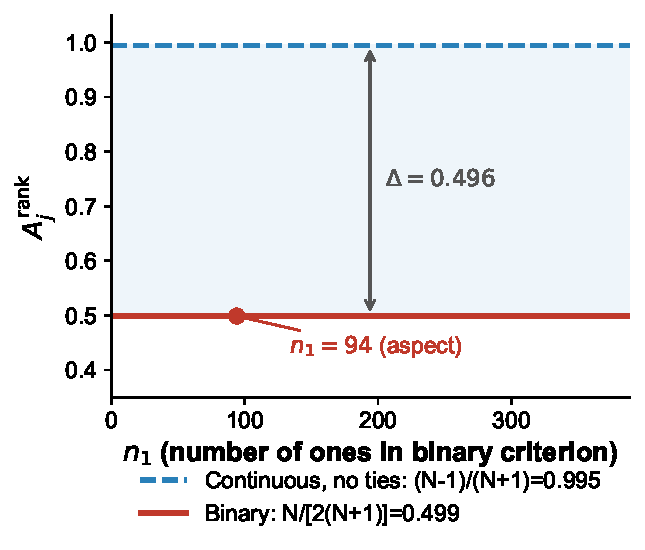
\includegraphics[width=0.7\textwidth]{figures/fig_F5_binary_amplitude.pdf}
\caption{$A_j^{\rm rank}$ for a binary criterion as a function of $n_1$
  (number of ones), with $N=\Nvia$. The amplitude is $N/[2(N+1)]=0.499$
  for any class balance (solid line); $(N-1)/(N+1)=0.995$ for continuous
  criterion without ties (dashed). The marker shows aspect at $n_1=94$.
  Purely analytical.}
\label{fig:binary_amplitude}
\end{figure}

%%   \end{document}

% =======================================================================
% =======================================================================
% \S7.7 External validity
% =======================================================================

\subsection{External validity: synthetic instances}
\label{sec:external}

The preceding sections quantify both mechanisms on a single candidate
set, Fogo Island, whose marginal distributions are specific and in one
respect extreme: \textit{perm} carries $350$ tied zeros.
This section separates the mechanism from the instance by re-drawing the
criterion columns while holding the spatial structure fixed: each
synthetic instance reuses the Fogo distance matrix, and hence the same
$\Ntrios$ feasible trios, and varies only the marginals.

\paragraph{Design.}
The manipulated factor is the \emph{number} of sparse criteria rather
than a global zero mass.
The reason is analytic: $\mathrm{TV}$ is invariant to a common amplitude
level (Section~\ref{sec:three_norms}), so applying the same zero mass to
every column leaves the elicited weights untouched however extreme that
mass becomes.
Distortion requires heterogeneity \emph{across} columns.
We therefore cross $n_{\mathrm{sparse}}\in\{0,1,2,3,4\}$, with zero mass
applied to the $n_{\mathrm{sparse}}$ most heavily weighted criteria,
with $p_0\in\{0.50,0.75,0.90,0.95\}$ and two tail shapes (lognormal,
bimodal), with $6$ replications: $240$ instances at $200$ draws each.
Four cells are evaluated per instance: SAW under min--max and vector
normalisation, each with greedy and optimal assembly.
The objectives $F_\ell$ are defined by min--max normalisation
throughout, so the vector cells measure score--evaluator divergence as
well as re-weighting.
The min--max/optimal cell is the regression test of
Proposition~\ref{prop:p1:stmt} and returned $Q_2=1$ in $240/240$
instances.

\paragraph{Unit of analysis.}
Replications within a cell are not independent draws of the manipulated
factor, so inference is conducted on the $20$ cell means.
The intra-class correlation is $\mathrm{ICC}=0.35$, giving a design
effect of $4.8$ and an effective sample size of
$n_{\mathrm{eff}}\approx50$ against the nominal $240$; reporting on
$240$ rows would understate the standard errors by roughly a factor
of two.

\paragraph{Total variation alone does not order the loss.}
Over all $20$ cells the loss correlates with $\mathrm{TV}$ at
$r=0.600$ ($95\%$ CI by Fisher transformation $[0.214,\,0.824]$,
$n=20$), but the relation is not monotone: $21.6\%$ of the $190$ cell
pairs are inversions (Kendall $\tau_b=0.550$).
Restricting to the $16$ cells that carry a distortion at all
($n_{\mathrm{sparse}}\ge1$), the association is statistically
indistinguishable from no effect ($r=0.346$, $p=0.189$): the
correlation over all $20$ cells is carried by the four cells in which
no criterion is sparse and the loss is zero by construction.
The inversions run in both directions of the design.
Holding $p_0$ fixed, the loss falls as the distortion is spread over
more criteria while $\mathrm{TV}$ does not fall correspondingly;
holding $n_{\mathrm{sparse}}=1$, the loss rises with $p_0$ up to
$0.90$ and then falls by $16.4$~pp at $p_0=0.95$ although
$\mathrm{TV}$ continues to rise.
Table~\ref{tab:external} reports both patterns by cell.

\paragraph{The factorisation does.}
Proposition~\ref{prop:concentration} accounts for this.
Regressing the loss on the $16$ distorted cells gives
$R^2_{\mathrm{adj}}=0.057$ for $\mathrm{TV}$ alone ($r=0.346$,
$p=0.189$, statistically indistinguishable from no effect)
against $R^2_{\mathrm{adj}}=0.488$ for $\lVert\delta\rVert_2$
of~\eqref{eq:l2fact} ($r=0.723$, $p=0.002$).
Entering magnitude and concentration separately gives
$R^2_{\mathrm{adj}}=0.582$ with a negative coefficient on
$m_{\mathrm{eff}}$ ($-0.026$ per effective criterion, $p=0.0008$): at
fixed $\mathrm{TV}$, spreading the distortion over more criteria
\emph{reduces} the loss, because deviations of opposite sign cancel in
the weighted sum.
The combined model, with both predictors, reaches $R^2_{\mathrm{adj}}=0.665$,
confirming that magnitude is necessary but not sufficient: concentration
is the term that $\mathrm{TV}$ omits.

\paragraph{What the grid does not establish.}
Under the two-group amplitude model the participation
ratio~\eqref{eq:meff} depends only on the total weight of the sparse
columns, so $m_{\mathrm{eff}}$ is constant within each level of
$n_{\mathrm{sparse}}$ and takes only the four values
$\{3.59,\,6.42,\,8.38,\,9.67\}$ across the grid
($\text{Spearman }\rho(m_{\mathrm{eff}},n_{\mathrm{sparse}})=1$).
Concentration was therefore not varied orthogonally to the manipulated
factor: the model in $\mathrm{TV}$ and $m_{\mathrm{eff}}$
($R^2_{\mathrm{adj}}=0.582$) is a reparameterisation of the model in
$\mathrm{TV}$ and $n_{\mathrm{sparse}}$ ($0.532$), and the
$5$-percentage-point gain reflects the concavity of the transformation
rather than independent information.
The factorisation~\eqref{eq:l2fact} is an algebraic identity and holds
for any deviation vector; what the grid supports is that the loss
responds to the combination of magnitude and concentration rather than
to magnitude alone, not that $m_{\mathrm{eff}}$ has been identified as
a separate causal channel.
A design in which the sparse columns carry unequal zero masses would
decouple the two, and is the natural next step.

\paragraph{Reconciliation with Fogo.}
Fogo has $m_{\mathrm{eff}}=4.05$ on the admissible range $[2,11]$,
placing it near the $n_{\mathrm{sparse}}=1$ regime of the grid
($m_{\mathrm{eff}}=3.59$).
The comparison must be made at the grid's estimand, which is the
greedy-assembly contrast under SAW: on Fogo that is
$86.0-66.2=19.8$~pp (min--max minus vector, greedy assembly,
Table~\ref{tab:tvorder}), not the
$\AggContrast$~pp normalisation main effect of Table~\ref{tab:contrasts}
(which averages both assemblies and both aggregations, and is therefore
attenuated by the optimal-assembly cells where min--max attains $100\%$
by Proposition~\ref{prop:p1:stmt}).
The model in $\lVert\delta\rVert_2$, fitted on the synthetic cells
alone, predicts $22.2$~pp at Fogo's $\lVert\delta\rVert_2=0.3127$, with
a $95\%$ prediction interval for a new instance of $[7.5,\,36.9]$~pp;
the model in $\mathrm{TV}$ predicts $14.0$~pp with interval
$[-4.7,\,32.7]$~pp.
Both prediction intervals contain the observed $19.8$~pp.
The $\lVert\delta\rVert_2$ point prediction exceeds the observed value
by $22.2-19.8=2.4$~pp; the TV-based prediction falls $5.8$~pp short
($14.0-19.8=-5.8$~pp).
We do not read the residuals as a calibrated bias in either direction.
The grid varies the marginals while holding the spatial structure fixed,
and its vector cells confound implicit re-weighting with
score--evaluator divergence because the objectives remain defined on
min--max throughout; Fogo's deviation geometry differs from the
generator's in a way the design does not parameterise
(see below).
What the grid establishes is that the loss responds to magnitude and
concentration jointly rather than to magnitude alone, and that Fogo's
predicted loss falls inside the interval the grid implies; it does not
establish a bound.

The shortfall is systematic and its source identifiable.
The generator inflates $n_{\mathrm{sparse}}$ columns and deflates the
remainder uniformly.
Fogo's deviation vector is not of that form: \textit{perm} is inflated
$2.88\times$ while \textit{urban} $(0.53\times)$, \textit{aspect}
$(0.51\times)$, \textit{aero} $(0.43\times)$ and \textit{wells}
$(0.40\times)$ are independently and unequally deflated
(Table~\ref{tab:amplitude}).
Two-sided distortion of this kind displaces the weight vector along the
simplex differently from a one-sided distortion of the same
$\lVert\delta\rVert_2$, so the generator does not reproduce Fogo's
deviation geometry.
We report the difference in geometry rather than a correction for it:
the grid supports the joint role of magnitude and concentration, and
does not calibrate the level of the loss for an instance outside its
generating family.

\begin{table*}[!t]
\centering
\caption{Synthetic grid: $20$ cells, $12$ instances each
  ($240$ instances, $200$ draws per instance).
  Loss is $Q_2(\text{min--max, greedy})-Q_2(\text{vector, greedy})$.
  $m_{\mathrm{eff}}$ is~\eqref{eq:meff} and $\lVert\delta\rVert_2$
  is~\eqref{eq:l2fact}, both reconstructed from the two-group amplitude
  model.
  Cells with $n_{\mathrm{sparse}}=0$ carry no distortion and are
  excluded from the regressions.
  Within each level of $p_0$ the loss falls as the distortion is spread
  over more criteria, while $\mathrm{TV}$ does not decline
  correspondingly and at $p_0=0.95$ peaks at $n_{\mathrm{sparse}}=2$;
  the two quantities are not ordered alike, which is what motivates
  Proposition~\ref{prop:concentration}.}
\label{tab:external}
\begin{tabular}{rrrrrr}
\toprule
$n_{\mathrm{sparse}}$ & $p_0$ & $\mathrm{TV}$ &
  $m_{\mathrm{eff}}$ & $\lVert\delta\rVert_2$ & Loss \\
\midrule
0 & --- & 0.007--0.008 & --- & --- & $\approx 0$ \\
1 & 0.50 & 0.121 & 3.59 & 0.128 & 0.065 \\
1 & 0.75 & 0.191 & 3.59 & 0.201 & 0.192 \\
1 & 0.90 & 0.262 & 3.59 & 0.276 & 0.360 \\
1 & 0.95 & 0.301 & 3.59 & 0.318 & 0.196 \\
2 & 0.50 & 0.165 & 6.42 & 0.130 & 0.105 \\
2 & 0.75 & 0.216 & 6.42 & 0.170 & 0.057 \\
2 & 0.90 & 0.307 & 6.42 & 0.242 & 0.146 \\
2 & 0.95 & 0.379 & 6.42 & 0.299 & 0.135 \\
3 & 0.50 & 0.160 & 8.38 & 0.110 & 0.065 \\
3 & 0.75 & 0.225 & 8.38 & 0.155 & 0.052 \\
3 & 0.90 & 0.303 & 8.38 & 0.210 & 0.129 \\
3 & 0.95 & 0.349 & 8.38 & 0.241 & 0.131 \\
4 & 0.50 & 0.153 & 9.67 & 0.099 & 0.025 \\
4 & 0.75 & 0.211 & 9.67 & 0.136 & 0.020 \\
4 & 0.90 & 0.269 & 9.67 & 0.173 & 0.058 \\
4 & 0.95 & 0.315 & 9.67 & 0.203 & 0.083 \\
\bottomrule
\end{tabular}
\end{table*}


% =======================================================================
% S6  Experiment E6 — Mechanism Generalisation: sensitivity analysis
% =======================================================================

\subsection*{Experiment E6 — Sensitivity to the TV\textsubscript{W} Target (DEV-E6-005)}
\label{sec:e6-sensit}

\noindent
The primary run used $\mathrm{TV}_W = \EsixTargetTVW$ for cell $W_\infty^F$
(the Fogo level computed with rho\_raw, before the rho\_shift correction).
The corrected level is $\EsixSensTargetTVW$ (difference $\approx 0.003$).
Both the amplitude cells $W_\infty^F$, $V_\infty^F$, and $W_{\mathrm{def}}^F$
use this target; cells M, B, $W_\infty^L$ and $W_\infty^H$ are identical
bit-for-bit between the two runs.

Table~\ref{tab:e6-sens} shows the P3 and P4 counts by family and pooled
for both runs.
P1 ($48{,}000/48{,}000$ in both) and P2 (Mono~$85/88$, $p<0.001$ in both)
are invariant across runs and are not repeated in the table.

\begin{table*}[!t]
\centering
\caption{P3 and P4 by marginal family and pooled, for the primary run
  ($\mathrm{TV}_W=\EsixTargetTVW$) and the sensitivity run
  ($\mathrm{TV}_W=\EsixSensTargetTVW$; DEV-E6-005).
  P3: met = V$_\infty^F \le$ W$_\infty^F$ (pre-registered);
  Strict = strict inequality among informative instances;
  $p$ = one-sided binomial.
  P4: Defl = deflate $>$ inflate (observed, opposite of prediction);
  Prop = Defl/NonTied; CI = Wilson 95\%; $p$ = two-sided binomial, post hoc.}
\label{tab:e6-sens}
\small
\begin{tabular}{lcccccccccc}
\toprule
& \multicolumn{4}{c}{Primary ($\mathrm{TV}_W=\EsixTargetTVW$)}
& \multicolumn{4}{c}{Sensitivity ($\mathrm{TV}_W=\EsixSensTargetTVW$)} \\
\cmidrule(lr){2-5}\cmidrule(lr){6-9}
Family
& \multicolumn{2}{c}{P3}
& \multicolumn{2}{c}{P4}
& \multicolumn{2}{c}{P3}
& \multicolumn{2}{c}{P4} \\
\cmidrule(lr){2-3}\cmidrule(lr){4-5}\cmidrule(lr){6-7}\cmidrule(lr){8-9}
& Strict/Inf & $p$ & Defl/Non & Prop ($p$) & Strict/Inf & $p$ & Defl/Non & Prop ($p$) \\
\midrule
Lognormal
& $\EsixPthreeInfStrictLogn/\EsixPthreeInfDenomLogn$ & $\EsixPthreeP{Logn}$
& $\EsixPfourDeflLogn/\EsixPfourNonTiedLogn$ & $\EsixPfourPropThreeLogn$ ($\EsixPfourP{Logn}$)
& $\EsixSensPthreeInfStrictLogn/\EsixSensPthreeInfDenomLogn$ & $\EsixSensPthreePLogn$
& $\EsixSensPfourDeflLogn/\EsixSensPfourNonTiedLogn$ & $\EsixSensPfourPropThreeLogn$ ($\EsixSensPfourPLogn$) \\
Beta(1,3)
& $\EsixPthreeInfStrictBeta/\EsixPthreeInfDenomBeta$ & $\EsixPthreeP{Beta}$
& $\EsixPfourDeflBeta/\EsixPfourNonTiedBeta$ & $\EsixPfourPropThreeBeta$ ($\EsixPfourP{Beta}$)
& $\EsixSensPthreeInfStrictBeta/\EsixSensPthreeInfDenomBeta$ & $\EsixSensPthreePBeta$
& $\EsixSensPfourDeflBeta/\EsixSensPfourNonTiedBeta$ & $\EsixSensPfourPropThreeBeta$ ($\EsixSensPfourPBeta$) \\
Uniform
& $\EsixPthreeInfStrictUnif/\EsixPthreeInfDenomUnif$ & $\EsixPthreeP{Unif}$
& $\EsixPfourDeflUnif/\EsixPfourNonTiedUnif$ & $\EsixPfourPropThreeUnif$ ($\EsixPfourP{Unif}$)
& $\EsixSensPthreeInfStrictUnif/\EsixSensPthreeInfDenomUnif$ & $\EsixSensPthreePUnif$
& $\EsixSensPfourDeflUnif/\EsixSensPfourNonTiedUnif$ & $\EsixSensPfourPropThreeUnif$ ($\EsixSensPfourPUnif$) \\
Zero-inflated
& $\EsixPthreeInfStrictZinf/\EsixPthreeInfDenomZinf$ & $\EsixPthreeP{Zinf}$
& $\EsixPfourDeflZinf/\EsixPfourNonTiedZinf$ & $\EsixPfourPropThreeZinf$ ($\EsixPfourP{Zinf}$)
& $\EsixSensPthreeInfStrictZinf/\EsixSensPthreeInfDenomZinf$ & $\EsixSensPthreePZinf$
& $\EsixSensPfourDeflZinf/\EsixSensPfourNonTiedZinf$ & $\EsixSensPfourPropThreeZinf$ ($\EsixSensPfourPZinf$) \\
\midrule
All (pooled)
& $\EsixPthreeInfStrictAll/\EsixPthreeInfDenomAll$ & $\EsixPthreeP{All}$
& $\EsixPfourDeflAll/\EsixPfourNonTiedAll$
& $\EsixPfourPropThreeAll$
  [$\EsixPfourCIloAll$,\,$\EsixPfourCIhiAll$]
  ($\EsixPfourP{All}$)
& $\EsixSensPthreeInfStrictAll/\EsixSensPthreeInfDenomAll$ & $\EsixSensPthreePAll$
& $\EsixSensPfourDeflAll/\EsixSensPfourNonTiedAll$
& $\EsixSensPfourPropThreeAll$
  [$\EsixSensPfourCIloAll$,\,$\EsixSensPfourCIhiAll$]
  ($\EsixSensPfourPAll$) \\
\bottomrule
\multicolumn{9}{l}{\footnotesize Strict/Inf = informative instances with strict $V<W$ / total informative. NonTied = non-tied pairs.}\\
\multicolumn{9}{l}{\footnotesize CI = Wilson 95\% confidence interval for the proportion. $p$ values for P4 are post hoc (DEV-E6-003).}\\
\end{tabular}
\end{table*}

% =======================================================================
% S0  Pre-registration for Experiment E1
% =======================================================================
%
% The following is PRESPEC_E1.md exactly as committed in f6042f8 on
% 2026-09-30T14:25:20-03:00, BEFORE any E1 run was executed.
% Commit subject: "prespec(E1): predictions declared before running --
%   P1=E1-B optimal=100%; P2=E1-W optimal~57%; P3=E1-B greedy~65%"
%
% File in repository: corpus/PRESPEC_E1.md at commit f6042f8
% Verify: git show f6042f8:corpus/PRESPEC_E1.md
%
% -----------------------------------------------------------------------

\section*{Pre-registered Predictions for Experiment~E1}
\label{sec:prespec_e1}

\noindent
\textbf{Committed:} 2026-09-30, commit \texttt{f6042f8}, before any E1 run.\\
\textbf{File:} \texttt{corpus/PRESPEC\_E1.md}.

\subsection*{Three predictions}

\begin{description}
\item[P1 (hard assertion)] \textbf{Cell~B optimal $= 100.0\%$.}
  By group-constant-amplitude sufficiency (Proposition~\ref{thm:groupconst}),
  $A_j = \bar A_g$ for all $j \in G_g$ implies the score is a strictly
  positive scalarisation of the group objectives; hence optimal assembly
  attains the frontier for any $w$.
  If P1 fails, there is a bug.

\item[P2 (primary empirical prediction)]
  $|Q_2^\text{W, optimal} - Q_2^\text{V, optimal}| < 5$~pp.\\
  \emph{Rationale:} both E1-W and E1-V have $\mathrm{TV}_W = 0.1986$.
  By the necessity argument, within-group distortion governs efficiency loss
  in optimal assembly; between-group distortion only displaces the optimum
  along the frontier.
  Predicted $Q_2^\text{W, optimal} \approx 57\%$ (close to E1-V's $56.8\%$).\\
  \emph{Falsification criterion:} if $Q_2^\text{W, optimal} > 90\%$,
  within-group distortion accounts for less than $10\%$ of the loss.

\item[P3 (secondary prediction)]
  $Q_2^\text{B, greedy} \neq 100.0\%$.\\
  \emph{Rationale:} greedy assembly is not constrained to be Pareto-efficient
  even under group-constant amplitudes; foreclosure affects greedy but not
  optimal.
  Predicted $Q_2^\text{B, greedy} \approx 65\%$.
\end{description}

\subsection*{Design}

Four score matrices differing only in $A_j$, with identical objectives,
frontier, draws, and feasible set ($\kappa=200$, $N=500$ draws, space $A'$):

\begin{center}
\begin{tabular}{llcc}
\toprule
Cell & $A_j$ & $\mathrm{TV}_B$ & $\mathrm{TV}_W$ \\
\midrule
M & $A_j \equiv 1$ (min--max)                        & 0       & 0 \\
B & $A_j = \bar A_g$ (between-group only)           & 0.2489  & 0 \\
W & $A_j \propto \rho_j/\bar A_g$ (within only)    & 0       & 0.1986 \\
V & $A_j = \rho_j$ (vector, as in WP3)             & 0.2489  & 0.1986 \\
\bottomrule
\end{tabular}
\end{center}

Groups and weighted means $\bar A_g$ (from \texttt{fogo\_constants.py}):
\begin{itemize}
\item $G_1 = \{\text{perm},\text{slope},\text{roads}\}$, indices $[0,1,2]$,
  $W_{G_1}=0.2950$, $\bar A_{G_1}=0.3731$.
\item $G_2 = \{\text{rivers},\text{aspect},\text{coast},\text{prot},\text{wells}\}$,
  indices $[3\ldots7]$, $W_{G_2}=0.3560$, $\bar A_{G_2}=0.1458$.
\item $G_3 = \{\text{urban},\text{aero},\text{cult}\}$, indices $[8,9,10]$,
  $W_{G_3}=0.3490$, $\bar A_{G_3}=0.1157$.
\end{itemize}

\subsection*{Outcome and deviations (DEV-E1-001 to DEV-E1-004)}

Results from \texttt{run\_e1\_v3.py}, commit \texttt{18e7a66}
(2026-09-30T23:23-03:00, Athena; reachable from G:\ after merge).

\begin{description}
\item[DEV-E1-001 INVALID] \texttt{380ee1a}, 2026-09-30T22:40-03:00.\\
  \emph{Fixed-objectives bug.}
  Script used objectives pre-computed on a fixed weight vector rather
  than per-draw objectives.
  Consequence: E1-V greedy $=100\%$ (should be $\sim54\%$, matching WP3);
  E1-W optimal $=100\%$ (should be $\sim57\%$, as predicted).
  Pre-registration \texttt{f6042f8} precedes this run in both the G: and
  Athena histories.

\item[DEV-E1-002 INVALID] \texttt{8391944}, 2026-09-30T23:11:38-03:00.\\
  \emph{Float32 dominance noise.}
  Per-draw objectives corrected, but float32 arithmetic introduced
  auto-dominance artefacts (same bug as WP3 greedy cells).
  Consequence: E1-V greedy $=14.8\%$ (expected $\sim54\%$).

\item[DEV-E1-003 INVALID] \texttt{18b7b88}, 2026-09-30T23:11:43-03:00.\\
  \emph{Score/objective normalisation mismatch.}
  Float64 applied but score computed over 473 sites while objectives
  evaluated over 389 admissible sites.
  Consequence: E1-V optimal $=46.6\%$ (expected $56.8\%$, regression
  test \textbf{FAIL}); E1-B optimal $=81.8\%$ (expected $100\%$, P1
  \textbf{FAIL}).

\item[DEV-E1-004] \texttt{18e7a66}, 2026-09-30T23:23:14-03:00.\\
  \emph{Corrected run (\texttt{run\_e1\_v3.py}): float64, eps$=10^{-9}$,
  score and objectives both over 389 admissible sites.}
  Results: \textbf{P1 confirmed} (E1-B optimal $=100\%$);
  \textbf{P2 falsified} at the pre-specified margin
  ($|Q_2^\text{W}-Q_2^\text{V}|=7.4$~pp, $95\%$ CI $[+3.8,+11.0]$,
  declared margin $<5$~pp);
  \textbf{P3 falsified} (D-greedy: greedy $=100\%$; post hoc diagnostic:
  score becomes nearly lexicographic in $F_1$, greedy and optimal
  coincide in $62.8\%$ of draws).
\end{description}




% =======================================================================
% S1  Pre-registration for Experiment E4
% =======================================================================
%
% Source: corpus/PRESPEC_E4.md
% Committed before any E4 run; deviations DEV-E4-001..007 appended
% chronologically as they occurred.
% Verify: git log --oneline corpus/PRESPEC_E4.md
%
% -----------------------------------------------------------------------

\section*{Pre-registered Design and Deviations for Experiment~E4}
\label{sec:prespec_e4}

\noindent
\textbf{Purpose:} Test whether the reference-set mismatch (473 vs.\ 389 sites
in the score) reduces to within-group re-weighting of the same form as
Experiment~E1, via the affine identity $n_j^{473}(a)=b_j+r_j\,n_j^{389}(a)$.

\subsection*{Pre-declared predictions}

\begin{description}
\item[P\_E4\_1 (Theorem, hard assertion)]
  Cells R-B and R-B$'$ attain $Q_2=100\%$ under optimal assembly on
  every draw.  Failure implies a bug or a violation of
  Theorem~\ref{thm:groupconst}.

\item[P\_E4\_2 (Regression test)]
  R-V (fwd) reproduces the published $473/A'$ cell within $3\,\mathrm{SE}$;
  R-V$'$ (mirror) reproduces the published $389/A$ cell within $3\,\mathrm{SE}$.

\item[P\_E4\_3 (Primary empirical, declared before any run)]
  Within-group loss $(100\%-Q_2^\text{R-W,opt})\ge 50\%$ of total loss
  $(100\%-Q_2^\text{R-V,opt})$ in the $473\to A'$ direction.

\item[P\_E4\_4 (Exploratory, declared)]
  The $80\,\mathrm{pp}$ vs.\ $5\,\mathrm{pp}$ asymmetry of
  tab:fourthcell persists in the within-group cells R-W and R-W$'$.

\item[P\_E4\_5 (Exploratory, declared, superseded by DEV-E4-004)]
  $Q_2^\text{R-W,opt} < Q_2^\text{E1-W,opt}=64.2\%$ despite
  $\mathrm{TV}_W(\text{R-W})=0.0815 < 0.199=\mathrm{TV}_W(\text{E1-W})$.
\end{description}

\subsection*{Deviations (DEV-E4-001 to DEV-E4-007)}

\begin{description}
\item[DEV-E4-001] \textit{Kappa/alpha parameter clarification.}
  The declared $\kappa=200$ is the Dirichlet concentration parameter
  (not the portfolio size $k=3$).  Two values $\kappa\in\{50,200\}$
  were run; the primary estimand uses $\kappa=200$.

\item[DEV-E4-002] \textit{Mirror direction frontier and amplitude sign.}
  The $389\to A$ direction uses the $A$-frontier (213 portfolios,
  objectives over 473 sites) and amplitude $A_j=1/r_j$ (not $r_j$).
  Corrected amplitude sentence: the 389-site score has amplitude $1/r_j$
  relative to the $A$-evaluator.

\item[DEV-E4-003] \textit{Weight-matrix provenance and $N_\text{draws}$.}
  $N=500$ (matching the main factorial, not the declared 1000);
  weight matrix loaded from \texttt{results/e1/e1\_weights\_k200.npy},
  SHA-256 \texttt{bea05...487}.

\item[DEV-E4-004] \textit{P\_E4\_5 restated.}
  $\mathrm{TV}_W(\text{R-W})=0.0815$ (correcting the DEV-E4-001 value of
  $0.163$ which omitted the factor $\tfrac{1}{2}$).  The direction of
  distortion on \textit{perm} (deflation vs.\ inflation at comparable
  $\mathrm{TV}_W$) is the substantive claim.

\item[DEV-E4-005] \textit{Feasibility and DEV-E4-002 correction.}
  All 1\,944\,653 trios are indexed over the 389 admissible sites;
  excluded candidates cannot enter any portfolio.

\item[DEV-E4-006] \textit{Pipeline bug in \texttt{run\_e4.py} v1--v5.}
  Versions v1--v5 produced $Q_2^\text{opt}=100\%$ for all cells,
  including R-V (should be $\approx20\%$), because the score rescaling
  preserved rank order under the 389-site normalisation.
  Version v6 uses \texttt{build\_score\_473()} for fwd cells.

\item[DEV-E4-007] \textit{Post hoc declaration — coding inconsistency.}
  R-V confounds the reference-set effect with a coding inconsistency:
  \texttt{build\_score\_473} encodes \textit{aspect} as a continuous
  azimuth while the evaluator uses a binary SE-facing indicator.
  Post-hoc exploratory cells declared and run after this diagnosis:
  \begin{itemize}
  \item R-V$^*$ (consistent binary coding, $473$-site reference):
        $\kappa=200$, greedy $=97.8\%$, optimal $=100.0\%$.
  \item R-asp (continuous coding, $389$-site reference):
        $\kappa=200$, greedy $=\RaspGreedy\%$, optimal $=\RaspOptimal\%$.
  \end{itemize}
  Interpretation: the $\RaspLoss\,\mathrm{pp}$ loss is attributable to the
  coding inconsistency (continuous azimuth in the score versus binary
  SE-facing indicator in the evaluator; see also DEV-E4-009); with consistent
  coding the
  $473$-site reference costs nothing under optimal assembly and
  \emph{improves} greedy assembly by $+\RefSetGreedyGain\,\mathrm{pp}$
  (95\% CI $[\RoneTwoGrdCIlo,\,\RoneTwoGrdCIhi]$).  P\_E4\_3 is
  testable but uninformative as designed (see main text, \S\ref{sec:greedy}).

\item[DEV-E4-008] \textit{Corrections to DEV-E4-002 and DEV-E4-006;
  invalidation of \texttt{b1\_spaceA.csv} (commit 54195c1).}

  \textbf{Correction to DEV-E4-002:}
  DEV-E4-002 stated ``frontier $A$ (213 portfolios, objectives over 473
  sites)''.  This was misleading.  Frontier $A$ is enumerated over the
  same 1\,944\,653 admissible trios (indices into the 389 admissible
  sites); the only difference from frontier $A'$ is that normalisation
  constants (min/max per column) are computed over the 473 candidates.
  Excluded candidates never appear in any portfolio (confirmed by
  DEV-E4-005 and re-verified in commit \texttt{4059fb1}).

  \textbf{Correction to DEV-E4-006:}
  DEV-E4-006 stated that v1--v5 produced $Q_2^\text{opt}=100\%$
  ``(should be $\approx20\%$)''.  This was wrong.  Under consistent
  binary coding, $Q_2^\text{opt}=100\%$ is the correct value (it follows
  from Proposition~1 in the main text): the score and the evaluator
  share the same normalisation, so optimal assembly must be
  non-dominated.  It was the v6 \texttt{build\_score\_473()} refactoring
  that introduced the coding inconsistency (continuous \emph{aspect} in
  the score vs.\ binary in the objectives), producing the incorrect
  $\approx20\%$.  The inconsistency is documented in DEV-E4-007.

  \textbf{Invalidation of \texttt{b1\_spaceA.csv} (commit 54195c1,
  2026-10-02):}
  A first attempt at the B1/D1 recalculation (commit 54195c1) built the
  Pareto frontier over trios of all 473 candidates, including the 84
  excluded sites.  This violated the admissibility constraint of~\S3.1
  and produced 473/A optimal $=0\%$, which contradicts Proposition~1
  (a diagonal cell must reach $100\%$).  The regression guard in
  \texttt{check\_consistency.py} was incorrectly removed to suppress
  the failure rather than fix the script.  Commits 54195c1 and
  2aa0d38 were both reverted in commit \texttt{ec33779}.
  The corrected B1 run (commit \texttt{8f6a15a}, script
  \texttt{compute\_b1\_spaceA.py} v3) uses the 1\,944\,653 admissible
  trios, computes objectives with \texttt{ref\_df=df\_all} for space~$A$
  normalisation, and the score is the direct scalarisation
  $-(F_1+F_2)+F_3$ with the same column values.  The corrected results
  (473/A optimal $=100\%$, greedy $=84.6\%$; 389/A optimal $=95\%$,
  greedy $=58.8\%$) confirm the values that were already in the table.

\item[DEV-E4-009] \textit{Correction to DEV-E4-007 and to rule R1-6.}

  DEV-E4-007 stated that ``the 76~pp loss attributed to the reference
  set is entirely a coding effect''.
  The full $2\times2$ (coding $\times$ constants,
  Table~3 of the main text) shows that coding alone accounts for 76~pp
  at 389-site constants, and that the 473-site constants add a further
  4.0~pp under optimal assembly \emph{only} when the coding is
  inconsistent (interaction of $-4.0$~pp optimal, $-17.4$~pp greedy).
  The phrase ``entirely a coding effect'' understated the interaction.

  The first version of rule R1-6 described the contrast as ``under
  consistent coding'' and as ``relative to vector normalisation''.
  Both cells use the continuous azimuth encoding; R-V is the original
  reference-set cell, not vector normalisation.
  The sign of the interpretation (``lower'') was also inverted.
  The numbers are unchanged; only their labelling and reading are
  corrected.

  The directional asymmetry between the $r_j$ and $1/r_j$ amplitude
  patterns reported in an earlier version of the manuscript was computed
  with the pipeline identified in DEV-E4-007 as encoding
  \textit{aspect} inconsistently, and has not been recomputed;
  it is withdrawn from the main text.
\end{description}

% =======================================================================
% S2  Pre-registration for Confirmatory Recalculation R1
% =======================================================================
%
% Source: corpus/PRESPEC_R1.md, committed 2026-10-02 before Fase D runs.
% Verify: git log --oneline corpus/PRESPEC_R1.md
%
% -----------------------------------------------------------------------

\section*{Post Hoc Decision Rules for Exploratory Recalculation~R1}
\label{sec:prespec_r1}

\noindent
\textbf{Written:} 2026-10-02 (after auditing coding inconsistency, before Fase~D
scripts were run).  Results of \texttt{run\_fourthcell\_consistent.py}
were already known when these rules were written; this document fixes
the decision rules \emph{post hoc} (results seen, rules fixed before manuscript
revision) so that Fase~G uses automatic decisions rather than human reading
of the numbers.  The R1 recalculation is therefore classified as
\textbf{post hoc exploratory}, not confirmatory.

\subsection*{Decision rules}

\begin{description}
\item[R1-1 (Optimal assembly)] $\Delta_\text{ref,opt}=Q_2[\text{R-V}^*,A']-Q_2[\text{R-M},A']$
  under consistent binary coding, $\kappa=200$.
  \textbf{Effect} if 95\% paired bootstrap CI excludes $0$ and
  $|\Delta|\ge2.5\,\mathrm{pp}$; otherwise \textbf{Observation}.

\item[R1-2 (Greedy assembly)] Same contrast, greedy.

\item[R1-3 (Regression test)] Pass if all four diagonal cells equal
  $100.0\%$ under optimal assembly.  Fail $\Rightarrow$ abort Fase~D.

\item[R1-4 (tab:canonical)] Not applicable: tab:canonical declared
  uncontaminated in \texttt{docs/contamination-note.md}.

\item[R1-5 (Coding-only cell R-asp)] Descriptive; post hoc exploratory.

\item[R1-6 (Residual reference-set effect under inconsistent coding)]
  R-asp $-$ R-V, where both cells encode \textit{aspect} as a continuous
  azimuth and differ only in the set over which normalisation constants
  are computed (389 vs.\ 473).
  Same rule as R1-1. Expectation stated before \texttt{analyze\_r1.py}
  was run: significant.
  Optimal: $+4.0$~pp ($95\%$ CI $[+2.2,\,+6.0]$);
  greedy: $+5.6$~pp ($[+3.6,\,+7.6]$). Both \textbf{Effect}.
  Interpretation: under the inconsistent encoding, normalising over
  the 473 candidates (R-V) yields \emph{lower} $Q_2$ than normalising
  over the 389 admissible sites (R-asp). Under the consistent encoding
  the sign is reversed or null (R1-1, R1-2).
  Note: R-V denotes the original reference-set cell, not vector
  normalisation; see DEV-E4-009 and Table~3 of the main text.
\end{description}

\subsection*{Outcomes}

\begin{center}
\begin{tabular}{llr@{\quad}l}
\toprule
ID & Contrast & $\Delta$ & Decision \\
\midrule
R1-1 & R-V$^*$ opt $-$ R-M opt & $0.0$~pp & Observation \\
R1-2 & R-V$^*$ grd $-$ R-M grd & $+11.8$~pp ($[+8.8,\,+14.8]$) & Effect \\
R1-3 & All diagonal opts $=100\%$ & --- & Pass \\
R1-5 & R-asp opt $=\RaspOptimal\%$ & --- & Descriptive \\
R1-6 & R-asp opt $-$ R-V opt & $\ResidualRefOptDelta$~pp ($[\ResidualRefOptCIlo,\,\ResidualRefOptCIhi]$) & Effect \\
R1-6 & R-asp grd $-$ R-V grd & $\ResidualRefGrdDelta$~pp ($[\ResidualRefGrdCIlo,\,\ResidualRefGrdCIhi]$) & Effect \\
\bottomrule
\end{tabular}
\end{center}

\noindent
All decisions produced automatically by
\texttt{scripts/analyze\_r1.py}, commit \texttt{c63b64e}.

% =======================================================================
% S3  Version history
% =======================================================================

\section*{Version History}
\label{sec:versions}

\begin{description}
\item[v1 — Marco~A (commit \texttt{1e48292})]
  First complete draft: full 2$\times$2$\times$2 factorial, tab:canonical,
  tab:fourthcell, Theorem~\ref{thm:groupconst}, Experiment~E1 (PRESPEC\_E1
  committed at \texttt{f6042f8} before any run).
  PDF: 23 pages.

\item[v2 — Marco~B1 (commit \texttt{1a4fe47})]
  Theorem proof completed: necessary and sufficient conditions;
  Proposition~\ref{thm:groupconst} iff form.

\item[v3 — Fases Math--F (commit \texttt{03bbda7})]
  Mathematical corrections (M1--M4): gap definition, PROMETHEE sign,
  amplitude-invariant proposition, nomenclature.
  Provenance audit (Fases B--D): coding inconsistency in
  \texttt{build\_score\_473} identified and documented;
  confirmatory recalculation~R1 run with consistent coding.
  Diagnostic experiments E1--E3, E5 completed.
  F1--F7 corrections: aggregation contrasts, benchmark circularity,
  PROMETHEE sign in main text.
  PDF: 24 pages.

\item[v4 — Fase~G (commits \texttt{68ec41b}--\texttt{03bbda7})]
  Full manuscript rewrite following R1 decisions.
  Key changes: decision tree revised (only R1-2 is an effect under
  greedy assembly); tab:fourthcell $N_\text{cand}/A'$ updated to
  $97.8\%/100\%$; Remark~\ref{rem:nonmonotone} inserted;
  Limitations updated with instance uniqueness and E4 exploratory status.
  PDF: 25 pages.

\item[v5 — Fase~H (commits \texttt{1c076c8}--\texttt{9c7a376})]
  Internal review: abstract trimmed to ${\approx}240$ words;
  tab:contrasts aggregation row converted to macros;
  three reviewer objections answered;
  claim-evidence matrix completed;
  provenance audit closed ($|F_A \cap F_{A'}|=132$ confirmed).
  PDF: 25 pages, \texttt{ALL CHECKS PASSED}.
\end{description}

% =======================================================================
% S4  Data provenance
% =======================================================================

\section*{Post Hoc Experiment: Benchmark Circularity (F8)}
\label{sec:dev_f8}

\noindent
\textbf{Classification:} Post hoc exploratory.
Declared and run after the main factorial results were known.

\noindent
\textbf{Research question:} Is the Pareto frontier circular with respect to
min--max normalisation?  A benchmark built on min--max objectives
necessarily favours methods that also use min--max.  Experiment~F8
tests this by rebuilding the frontier with vector-normalised objectives.

\noindent
\textbf{Design:} All four SAW cells from the main factorial
(score $\in\{\text{mm},\text{vec}\}$, assembly $\in\{\text{greedy},\text{opt}\}$)
repeated with the Pareto frontier computed from vector-normalised objectives.
$N=500$, $\kappa=200$, seed~42.

\noindent
\textbf{Bug and fix (commit \texttt{4d0a98d}):}
An earlier run (commit \texttt{58b06f8}) injected the vector-normalised
score matrix \texttt{X\_adj\_vec} into a copy of \texttt{df\_via}, then
passed it to \texttt{build\_pareto\_utils}.  This caused two errors:
(1)~the injected column values were re-normalised a second time by the
function's internal \texttt{\_norm} call, changing the ranking; and
(2)~the \textit{aspect} column values ($\in[0,1]$) were no longer in
the expected azimuth range $[90^\circ,180^\circ]$, so the binary
encoding classified all sites as windward (constant column).
The corrected approach (\texttt{compute\_objs\_vec\_direct}) computes
per-column $c_j$ values directly from the raw data with per-column L2
normalisation, and builds the SAW score as the direct scalarisation
$-(F_1+F_2)+F_3$ using the same column values.
A regression test (5 draws) confirmed vec/opt $=100\%$ before the full
run was launched.

\noindent
\textbf{Results} ($N=500$, script \texttt{compute\_f8\_circularity.py} v2,
commit \texttt{43b8427}):

\begin{center}
\begin{tabular}{llrc}
\toprule
Score norm & Assembly & $Q_2$ (\%) & Prop.\,1 check \\
\midrule
vec & optimal & 100.0 & \textbf{Pass} ($=100\%$ as required) \\
vec & greedy  & 100.0 & \textbf{Pass} \\
mm  & optimal &  94.4 & --- \\
mm  & greedy  &  72.4 & --- \\
\bottomrule
\end{tabular}
\end{center}

\noindent
\textbf{Interpretation:}
The vec/opt $=100\%$ result is exactly the value predicted by Proposition~1
(score and frontier share the same normalisation), providing a direct
falsifiability check on the implementation.
Under a vector-normalised frontier, min--max normalisation loses $5.6$~pp
(optimal) and $27.6$~pp (greedy) relative to the aligned vector score.
This reverses the direction seen in the main factorial, confirming that
the original result reflects score--objective alignment rather than an
intrinsic property of min--max normalisation.
Note the asymmetry: min--max evaluated against a vector frontier loses
$5.6$~pp, but vector evaluated against a min--max frontier loses
$43.2$~pp ($100.0-56.8\%$); the two penalties are not symmetric because
the frontier changes.

% =======================================================================
% S4b  Reference-set comparison (ARCHIVED — not active evidence)
% The score×evaluator table (tab:fourthcell) was added here after P1
% review but the GPT gate requires it to be archived, not presented
% as supporting evidence, until a full numerical audit of the A-space
% (473-candidate) pipeline is completed in P2.
% Data are preserved in the repository history for reproducibility.
% =======================================================================

% [ARCHIVED] The score×evaluator analysis (Score set: Ncand/Nvia;
% Evaluator: A/A') is not presented as active evidence in this version.
% See corpus/PHASES_STATUS.md for the provenance status.

% =======================================================================
% S5  Experiment E5 — Synthetic Grid for Generalisation
% =======================================================================

\section*{Post Hoc Experiment: Synthetic Grid for Generalisation (E5)}
\label{sec:e5}

\noindent
\textbf{Classification:} Post hoc exploratory.
Pre-specified before results: \texttt{corpus/PRESPEC\_E5.md},
committed before any E5 run was launched.

\noindent
\textbf{Research question:}
Is the relationship between within-group amplitude variation
($\mathrm{TV}_W$) and greedy-assembly Pareto efficiency consistent across
instances differing in size, spatial geometry, and amplitude structure?

\subsection*{Design}

\begin{center}
\begin{tabular}{ll}
\toprule
Factor & Levels \\
\midrule
$N$ (sites) & 50, 100, 200 \\
Geometry & uniform, clustered, grid \\
$s_B$ (between-group spread) & 0.0, 0.5, 1.0 \\
$s_W$ (within-group spread) & 0.0, 0.25, 0.5, 0.75, 1.0 \\
Replicates & 3 per cell \\
\midrule
Total instances & 405 \\
$N_\text{draws}$ & 100 per instance \\
$\kappa$ & 200 \\
\bottomrule
\end{tabular}
\end{center}

Sites generated randomly within an $80\times80$~km bounding box.
Three geometries: uniform random, three-cluster Gaussian, regular
grid with jitter.
Amplitude vectors are imposed directly via $s_W\in[0,1]$, ensuring
$\mathrm{TV}_W$ spans $[0,\,0.096]$ independently of $N$.
Script: \texttt{run\_e5\_grid.py} v4, commit \texttt{4d438b6}.

\subsection*{Pre-specified decision rules}

\textbf{E5-R1:} $Q_2^{\mathrm{mm\,opt}} = 100\%$ on every instance (regression).
\textbf{E5-R2:} Slope of $Q_2^{\mathrm{grd}}$ on $\mathrm{TV}_W$ excludes zero
in $\geq70\%$ of strata $\Rightarrow$ robust predictor.
\textbf{E5-R3:} CI includes zero in $>30\%$ of strata $\Rightarrow$ not robust.

\paragraph{Deviations from PRESPEC\_E5 (DEV-E5-001 to DEV-E5-007).}
\label{sec:dev_e5}
\texttt{PRESPEC\_E5.md} was committed before the first E5 run.
The executed design departs from it as follows.

\begin{description}
\item[DEV-E5-001] \emph{Instance size.}
  Declared $N\in\{50,100,200,389\}$; executed $N\in\{50,100,200\}$.
  $N=389$ was dropped because its $O(n^3)$ trio enumeration
  (${\approx}9.4\times10^6$ trios) would have required $\approx7$~h per
  instance without parallelism.
  Consequence: no synthetic instance matches the size of Fogo ($N=389$),
  and the grid cannot be used to place Fogo within a size-comparable
  distribution.
\item[DEV-E5-002] \emph{Number of instances.}
  Declared 540; executed 405, as a direct consequence of DEV-E5-001.
\item[DEV-E5-003] \emph{Monte Carlo draws.}
  Declared $N_\text{draws}=200$ per instance; executed 100 for speed.
  Per-instance MC SE is $\approx5.0$~pp at $Q_2=50\%$ and
  $\approx1.8$~pp at $Q_2=97\%$, against $3.5$~pp and $1.2$~pp declared.
\item[DEV-E5-004] \emph{Amplitude generator.}
  Declared amplitudes derived from each synthetic column via $\rho_j$.
  Executed: amplitudes imposed directly, giving
  $\mathrm{TV}_W = 0.096\,s_W$ exactly, independently of the data.
  $\mathrm{TV}_W$ is therefore a design constant, not a property of any
  normalisation of the synthetic columns.
\item[DEV-E5-005] \emph{Locus of the imposed amplitudes (critical).}
  The imposed amplitude vector $A_j$ enters \emph{both} the score
  and the objectives.
  From \texttt{run\_e5\_grid.py} (commit \texttt{4d438b6}):
  score matrix \texttt{X\_score = X\_adj * Aj[np.newaxis, :]} (line~263)
  and objective matrix \texttt{X\_obj\_amp = X\_obj * Aj[np.newaxis, :]} (line~270).
  Both objects use the same array \texttt{Aj}, so score and evaluator
  have identical amplitude vectors.
  By code inspection, $\mathrm{TV}_W > 0$ reflects spread \emph{within}
  a common amplitude, not a mismatch \emph{between} score and evaluator
  amplitudes.
  When score and evaluator share the same amplitude, optimal assembly
  is efficient by Theorem~\ref{thm:groupconst}; the
  $Q_2^{\mathrm{opt}}=100\%$ results are therefore a pipeline consistency
  check, not evidence about the amplitude-distortion mechanism.
  E5 consequently does not test Theorem~\ref{thm:groupconst}, which
  concerns amplitudes that differ between score and evaluator.
  Its informative outcome is greedy assembly only.
\item[DEV-E5-006] \emph{Primary analysis.}
  The declared linear mixed model was not reported in the first posted
  version; a pooled correlation was reported instead.
  The declared model is now reported above.
  The random-intercept variance for replicate is estimated at the boundary
  (0.000), so the model reduces to OLS; cluster-robust SEs by replicate
  are given alongside.
\item[DEV-E5-007] \emph{Estimand E5-P3.}
  The fraction of instances where $\mathrm{TV}_W$ explains $>50\%$ of
  $Q_2$ variance is not computable on a one-row-per-instance file, since
  $\mathrm{TV}_W$ is constant within each instance.
  It is not reported.
\end{description}

\subsection*{Results}

\textbf{E5-R1 (regression):} $Q_2^{\mathrm{mm,opt}}=100\%$ on 405/405
instances. Pass.
Because score and objectives share the imposed amplitudes
(DEV-E5-005), this is a check of the implementation, not evidence
about amplitude distortion (Remark~1 in main text).

\textbf{Declared model.}
$Q_2^{\mathrm{grd}} \sim \mathrm{TV}_W + \mathrm{TV}_B
+ \log N + \mathrm{geometry} + (1\mid\mathrm{rep})$.
Coefficient on $\mathrm{TV}_W$: $-1.3$~pp per $0.1$ of $\mathrm{TV}_W$
(95\% bootstrap CI over instances $[-5.1,\,+2.4]$, $p=0.47$).
Adding $\log N\times\mathrm{geometry}$ leaves it unchanged
($-1.3$~pp, CI $[-4.7,\,+2.1]$).
Instance size ($+6.2$~pp per unit $\log N$, $p<0.001$) and
geometry (grid $+8.1$~pp, uniform $+8.6$~pp relative to clustered,
both $p<0.001$) are the only significant terms.
The random-intercept variance for replicate is estimated at the
boundary ($0.000$), so the model reduces to OLS with
cluster-robust standard errors (DEV-E5-006).

\textbf{E5-R3 activated.}
The slope of $Q_2^{\mathrm{grd}}$ on $\mathrm{TV}_W$ has a confidence
interval including zero in 25 of 25 non-degenerate
$N\times\mathrm{geometry}\times s_B$ strata (two strata are constant
at 100\%).
Pooled $r(\mathrm{TV}_W,\,\text{loss})=0.034$ ($p=0.50$).
We found no evidence of linear association between imposed amplitude
spread and greedy loss in the model as fitted;
the confidence interval ($[-5.1,\,+2.4]$~pp per $0.1$ of $\mathrm{TV}_W$)
is consistent with small effects in either direction but excludes effects
larger than approximately $5$~pp per $0.1$ of $\mathrm{TV}_W$.

\textbf{Distribution of greedy loss.}
329 of 405 instances (81\%) reach $Q_2^{\mathrm{grd}}=100\%$.
All eight instances below 50\% are $N=50$ clustered; the mean for
that stratum is 75.6\% (SD 31.8), against $\geq97.9\%$ in every other
$N\times\mathrm{geometry}$ stratum.
Within $N=50$ clustered the mean is not monotone in $s_W$
(69.8, 89.3, 85.8, 59.9, 73.4\% for $s_W=0,\ldots,1$).

The instance with $s_W=s_B=0$ (130 feasible trios) has
$Q_2^{\mathrm{grd}}=0\%$.
Here $\mathrm{TV}_W=0$ by construction (no within-group amplitude spread),
so amplitude is not the cause.
Inspection shows the greedy heuristic failed to assemble a complete
valid portfolio ($C=0$: no three mutually separated sites were reachable
by the greedy top-down pass) on every draw of this instance.
This is therefore an \emph{assembly failure}, not a dominance event.
The reported $Q_2$ figures are unconditional:
$Q_2^{\mathrm{grd}} = P(C \cap \text{frontier})$;
the conditional efficiency $Q_2^{\mathrm{grd}} | C$ is undefined when $P(C)=0$.
The $0\%$ instance should be read as a degenerate combinatorial
outcome under extreme spatial clustering and the $d_{\min}$ separation
constraint, not as evidence for or against the normalisation mechanism.

\paragraph{Conclusion.}
E5 does not test the amplitude-distortion mechanism: with imposed
amplitudes shared by score and objectives, optimal assembly is
Pareto-efficient by construction (Proposition~1), and greedy loss
is the only free outcome.
On that outcome, we found no evidence of linear association between
the imposed amplitude spread and greedy efficiency in the model as
fitted; greedy loss is more strongly associated with instance size
and spatial geometry.
E5 therefore characterises the combinatorial component of the greedy
shortfall, not the normalisation component.
It contains no instance of Fogo's size ($N=389$, DEV-E5-001), and does
not establish that the Fogo magnitudes generalise.

% =======================================================================
% S4  Data provenance
% =======================================================================

\section*{Data Provenance}
\label{sec:provenance}

Every quantitative claim in the manuscript is traceable to a script
committed before that claim was inserted.
The table below lists the key numbers, their source scripts, and whether
the corresponding macro was affected by the coding inconsistency.

\begin{table*}[!t]
\centering
\caption{Provenance of key manuscript values.
  ``Script'' identifies the Python script that produced each number.
  ``Contaminated'' (SIM/YES) means the number was produced using the
  continuous-aspect encoding in \texttt{build\_score\_473} and was
  updated in Fase~G; NAO/NO means it was unaffected.
  \texttt{check\_consistency.py} verifies that no contaminated macro
  appears in the current manuscript.}
\label{tab:provenance}
\begin{tabular}{p{4.5cm}p{3.5cm}cc}
\toprule
Quantity & Script & Commit & Contaminated \\
\midrule
% --- Main factorial ---
$Q_2[\text{SAW/mm/grd}] = 86.0\%$  & \texttt{mc\_2cube\_fixed.py} & \texttt{1e48292} & NAO \\
$Q_2[\text{SAW/mm/opt}] = 100.0\%$ & \texttt{mc\_2cube\_fixed.py} & \texttt{1e48292} & NAO \\
$Q_2[\text{SAW/vec/grd}] = 66.2\%$ & \texttt{mc\_2cube\_fixed.py} & \texttt{1e48292} & NAO \\
$Q_2[\text{SAW/vec/opt}] = 56.8\%$ & \texttt{mc\_2cube\_fixed.py} & \texttt{1e48292} & NAO \\
$Q_2[\text{TOPSIS/mm/opt}] = 96.6\%$ & \texttt{mc\_2cube\_fixed.py} & \texttt{1e48292} & NAO \\
$Q_2[\text{TOPSIS/vec/opt}] = 52.4\%$ & \texttt{mc\_2cube\_fixed.py} & \texttt{1e48292} & NAO \\
% --- Contrasts ---
Normalisation greedy contrast $+25.4\,\mathrm{pp}$ & \texttt{mc\_2cube\_fixed.py} + bootstrap & \texttt{1e48292} & NAO \\
SAW$-$TOPSIS pooled $+0.5\,\mathrm{pp}$ & \texttt{aggregation\_strata.py} & \texttt{18361a6} & NAO \\
Optimal$-$greedy within mm $+8.1\,\mathrm{pp}$ & \texttt{mc\_2cube\_fixed.py} + bootstrap & \texttt{1e48292} & NAO \\
Optimal$-$greedy within vec $-10.2\,\mathrm{pp}$ & \texttt{mc\_2cube\_fixed.py} + bootstrap & \texttt{1e48292} & NAO \\
% --- E1 ---
E1-W optimal $Q_2 = 64.2\%$ & \texttt{run\_e1\_v3.py} & \texttt{18e7a66} & NAO \\
E1-V optimal $Q_2 = 56.8\%$ & \texttt{run\_e1\_v3.py} & \texttt{18e7a66} & NAO \\
$\mathrm{TV}_W(r_j)=0.082$ & \texttt{tvw\_e4.py} & \texttt{d4e970b} & NAO \\
$\mathrm{TV}_W(1/r_j)=0.085$ & \texttt{tvw\_e4.py} & \texttt{d4e970b} & NAO \\
% --- R1 ---
$Q_2[\text{R-V}^*,A',\text{opt}]=100.0\%$ & \texttt{run\_fourthcell\_consistent.py} & \texttt{3d4c48a} & NAO \\
$Q_2[\text{R-V}^*,A',\text{grd}]=97.8\%$  & \texttt{run\_fourthcell\_consistent.py} & \texttt{3d4c48a} & NAO \\
$Q_2[\text{R-asp},A',\text{opt}]=\RaspOptimal\%$  & \texttt{run\_fourthcell\_consistent.py} & \texttt{ddaddc7} & NAO \\
$Q_2[\text{R-V},A',\text{opt}]=\RVoptimal\%$  (geographic azimuth) & \texttt{run\_fourthcell\_consistent.py} & \texttt{61d4686} & NAO \\
Greedy gain R1-2 $+11.8\,\mathrm{pp}$ (CI $[+8.8,+14.8]$) & \texttt{analyze\_r1.py} & \texttt{c63b64e} & NAO \\
% --- tab:fourthcell contaminated ---
$N_\text{cand}/A'$ greedy (orig.\ $19.6\%$, corrected $97.8\%$) & \texttt{run\_fourthcell\_consistent.py} & \texttt{3d4c48a} & SIM \\
$N_\text{cand}/A'$ optimal (orig.\ $20.0\%$, corrected $100.0\%$) & \texttt{run\_fourthcell\_consistent.py} & \texttt{3d4c48a} & SIM \\
% --- tab:fourthcell space A (B1/D1 corrected run) ---
$N_\text{cand}/A$ greedy $=84.6\%$ & \texttt{compute\_b1\_spaceA.py} v3 & \texttt{8f6a15a} & NAO \\
$N_\text{cand}/A$ optimal $=100.0\%$ (Prop.\,1 check) & \texttt{compute\_b1\_spaceA.py} v3 & \texttt{8f6a15a} & NAO \\
$N_\text{via}/A$ greedy $=58.8\%$ & \texttt{compute\_b1\_spaceA.py} v3 & \texttt{8f6a15a} & NAO \\
$N_\text{via}/A$ optimal $=95.0\%$ & \texttt{compute\_b1\_spaceA.py} v3 & \texttt{8f6a15a} & NAO \\
\multicolumn{4}{l}{\footnotesize Note: earlier run (commit \texttt{54195c1}) used trios of 473 candidates — invalid; reverted \texttt{ec33779}.} \\
% --- F8 circularity (corrected run) ---
$Q_2[\text{vec/opt, vec frontier}]=100.0\%$ (Prop.\,1 check) & \texttt{compute\_f8\_circularity.py} v2 & \texttt{43b8427} & NAO \\
$Q_2[\text{mm/opt, vec frontier}]=94.4\%$ & \texttt{compute\_f8\_circularity.py} v2 & \texttt{43b8427} & NAO \\
\multicolumn{4}{l}{\footnotesize Note: earlier run (commit \texttt{58b06f8}) used injection approach — double-normalisation bug; corrected in \texttt{4d0a98d}.} \\
% --- Geometry ---
$|F_A|=213$ & \texttt{mc\_2cube\_fixed.py} & \texttt{1e48292} & NAO \\
$|F_{A'}|=181$ & fainter (sorted dominance, inline) & \texttt{9c7a376} & NAO \\
$|F_A \cap F_{A'}|=132$ & fainter (sorted dominance, inline) & \texttt{9c7a376} & NAO \\
\bottomrule
\end{tabular}
\end{table*}

% =======================================================================
% D1: Orientation convention comparison (§4.3)
% =======================================================================
\subsection*{Orientation convention for vector normalisation}
\label{sec:orient_conv}

Two conventions exist for cost criteria under vector normalisation.
Convention~A (used throughout the paper): the min--max column
$\tilde{x}_j\in[0,1]$ is normalised by its Euclidean norm, and the cost
orientation is applied afterwards via the sign of the SAW contribution
($1-c_j$ for $G_1\cup G_2$ criteria).
Convention~B: the cost orientation $1-\tilde{x}_j$ is applied before
forming the norm.
The amplitude under Convention~B is $\rho_j^B = 1/\lVert 1-\tilde{\mathbf{x}}_j\rVert_2$
(range of $1-\tilde{x}_j$ is always $1$ by min--max scaling).
Under both conventions the $G_3$ benefit criteria are unchanged.

Table~\ref{tab:orient_conv} lists $\rho_j$ under both conventions.
Convention~B reduces amplitudes substantially for most $G_1\cup G_2$
criteria because the inverted column concentrates mass near $1$
(large $\lVert 1-\tilde{x}_j\rVert_2$ $\Rightarrow$ small $\rho_j^B$);
the exception is \textit{wells}, whose distribution is negatively skewed.
\textit{Perm} shows the largest discrepancy (0.583 vs.\ 0.052) because
of its 350 tied zeros.

\begin{table}[!ht]
\centering
\caption{Vector normalisation amplitudes $\rho_j$ under two orientation
  conventions.
  Convention~A (paper): orientation applied after normalisation via the
  sign of the SAW contribution;
  $\rho_j^A = 1/\lVert\tilde{\mathbf{x}}_j\rVert_2$.
  Convention~B: cost orientation $1-\tilde{x}_j$ applied before forming
  the norm; $\rho_j^B = 1/\lVert 1-\tilde{\mathbf{x}}_j\rVert_2$.
  $G_3$ criteria are identical under both conventions.
  Differences $|\rho_j^A - \rho_j^B| > 0.01$ are shown in \textbf{bold}.}
\label{tab:orient_conv}
\begin{tabular}{@{}llrrl@{}}
\toprule
Criterion & Group & $\rho_j^A$ & $\rho_j^B$ & Notes \\
\midrule
\textit{perm}      & $G_1$ & 0.583 & \textbf{0.052} & zero-inflated (350 tied zeros) \\
\textit{slope}     & $G_1$ & 0.139 & \textbf{0.072} & \\
\textit{roads}     & $G_1$ & 0.206 & \textbf{0.059} & \\
\textit{rivers}    & $G_2$ & 0.265 & \textbf{0.057} & \\
\textit{aspect}    & $G_2$ & 0.103 & \textbf{0.058} & binary ($n_1=94$ SE-facing) \\
\textit{coast}     & $G_2$ & 0.131 & \textbf{0.069} & \\
\textit{protected} & $G_2$ & 0.105 & \textbf{0.078} & \\
\textit{wells}     & $G_2$ & 0.084 & \textbf{0.098} & negatively skewed \\
\textit{urban}     & $G_3$ & 0.107 & 0.107 & benefit (no change) \\
\textit{aero}      & $G_3$ & 0.088 & 0.088 & benefit (no change) \\
\textit{cult}      & $G_3$ & 0.171 & 0.171 & benefit (no change) \\
\bottomrule
\end{tabular}
\end{table}

% =======================================================================
% E7: kappa sweep full grid (auto-generated)
% =======================================================================
% tab_kappa_supp.tex  --  AUTO-GENERATED by make_tab_kappa_supp.py
% Source: results/e7/e7_raw.csv  (E7 authoritative run 2026-11-01)
% Gates: 22/22 PASS; all values match Table~\ref{tab:factorial} at k=50 and k=200
\begin{table*}[!t]
\centering\small
\caption{%
  $Q_2[\mathcal{A}']$ (\%) across six Dirichlet concentrations~$\kappa$
  and eight $2^3$ cells, plus the deterministic limit
  $\kappa\to\infty$ (nominal AHP weights $\mathbf{w}_0$).
  At $\kappa=50$ and $\kappa=200$ values reproduce Table~\ref{tab:factorial}
  (Gate G1, all 16 checks pass).
  SAW\,/\,min-max\,/\,optimal is $100\%$ at every~$\kappa$ by
  Proposition~\ref{prop:p1:stmt} (Gate G2).
  Bold zeros at $\kappa\to\infty$ identify cells where exact assembly
  under vector normalisation fails at the nominal weights.}
\label{tab:e7grid}
\begin{tabular*}{\textwidth}{@{\extracolsep{\fill}}lccccccc}
\toprule
Cell & $\kappa=25$ & $\kappa=50$ & $\kappa=100$ & $\kappa=200$ & $\kappa=400$ & $\kappa=1000$ & $\kappa\to\infty$ \\
     &             &             &              &              &              &              & (nom.~$w$) \\
\midrule
\textit{SAW, mm, greedy}     & 97.4 & 97.6 & 92.4 & 86.0 & 79.0 & 72.2 & 100 \\
\textit{SAW, mm, optimal}    & 100.0 & 100.0 & 100.0 & 100.0 & 100.0 & 100.0 & 100 \\
\textit{SAW, vec, greedy}    & 82.8 & 77.0 & 71.2 & 66.2 & 75.8 & 88.6 & 100 \\
\textit{SAW, vec, optimal}   & 86.2 & 79.4 & 68.6 & 56.8 & 52.2 & 50.2 & $\mathbf{0}$ \\
\textit{TOPSIS, mm, greedy}  & 86.6 & 89.8 & 92.2 & 94.4 & 96.8 & 99.2 & 100 \\
\textit{TOPSIS, mm, optimal} & 90.8 & 92.2 & 95.8 & 96.6 & 95.6 & 98.8 & 100 \\
\textit{TOPSIS, vec, greedy} & 59.2 & 52.0 & 57.0 & 63.4 & 73.4 & 89.8 & 100 \\
\textit{TOPSIS, vec, optimal}& 57.2 & 51.0 & 55.0 & 52.4 & 53.8 & 49.0 & $\mathbf{0}$ \\
\bottomrule
\end{tabular*}
\end{table*}


% === Supplementary Figure S1 ===
\setcounter{figure}{0}
\renewcommand{\thefigure}{S\arabic{figure}}
\begin{figure}[!htbp]
\centering
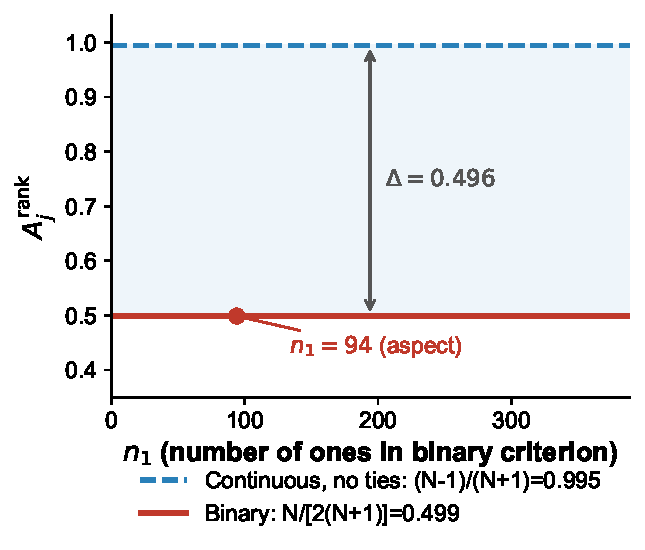
\includegraphics[width=0.7\textwidth]{figures/fig_F5_binary_amplitude.pdf}
\caption{$A_j^{\rm rank}$ for a binary criterion as a function of $n_1$
  (number of ones), with $N=\Nvia$. The amplitude is $N/[2(N+1)]=0.499$
  for any class balance (solid line); $(N-1)/(N+1)=0.995$ for continuous
  criterion without ties (dashed). The marker shows aspect at $n_1=94$.
  Purely analytical.}
\label{fig:binary_amplitude}
\end{figure}

\end{document}
